\documentclass[12pt,a4paper]{article}
 
\usepackage{float}
%für feststellen der figures und tables [H] dranschreiben
\usepackage{units}
%wird so benutzt: 
%\unit[value/Zahl]{dimension/Einheit} oder 
%\unitfrac[value/Zahl]{dimension/Einheit num/Zähler}{dimension/Einheit denum/Nenner} oder
%\nicefrac[fontcommand/Schriftart]{dimension/Einheit num/Zähler}{dimension/Einheit denum/Nenner}

\usepackage{caption}
\usepackage{subcaption}

\usepackage[left=2cm,right=2cm,top=2cm,bottom=2cm]{geometry}
\usepackage[utf8]{inputenc}
\usepackage[T1]{fontenc}
\usepackage{lmodern}
\usepackage[ngerman]{babel}
\usepackage{amsmath}
\usepackage{graphicx}
 
\title{Operationsverstärker}
\author{Frederik Strothmann, Henrik Jürgens}
\date{\today}
%niemals zwei überschriften direkt übereinander schreiben, also immer mindestens in einem satz was sinnvolles unter jede überschrift schreiben (bei den versuchen z.B. das versuchsziel) 
\begin{document}
%deckblatt erstellen.
\maketitle
\newpage
\tableofcontents
\newpage
\section{Einleitung}
%einleitung zu dem experiment.
%auf die einstellungen, die vor dem versuch gemacht werden, eingehen oder auf eine anleitung dazu verweisen
%es soll immer erwähnt werden um was es in dem Versuch geht und wie das relisiert werden soll
%---------------------------------------------------------------------------------------------
%hinter der einleitung kann der allgemeine theoretische hintergrund in einer zusätzlichen section erklärt werden
%1-----------------------------------------------1
In diesem Versuch geht es um den Operationsverstärker, einem wichtigen Bauelement der analogen Schaltungselektronik. (Op-Amp oder Operational Amplifier) Mit ihm lassen sich elektrische Verstärkungsschaltungen einfacher und mit besseren elektrischen Eigenschaften aufbauen, als mit einzelnen Transistoren möglich ist. Die Operationsverstärker TL071 und TL081 werden in verschiednen Schaltungen untersucht.
\section{Impedanzwandler für Gleichspannung}
%kurz das ziel dieses versuchsteiles ansprechen, damit keine zwei überschriften direkt übereinander stehen!
%bei schwierigeren versuchen kann auch der theoretische hintergrund erläutert werden. (mit formeln, herleitungen und erklärungen)
Es soll gezeigt werden, wie eine Spannungsquelle mit hohem Innenwiderstand in eine Spannungsquelle mit einem relativ niedrigem Innenwiderstand von ca. \unit[100]{$\Omega$} umgewandelt werden kann. Dies geschieht über den sog. 'Impedanzwandler'.
\subsection{Verwendete Materialien}
%(immer) eine skizze oder ein foto einfügen, die geräte/materialien !nummerieren! und z.b. eine legende dazu schreiben, besser wäre es das ganze in einem Fließtext gut zu beschreiben.
%falls am anfang des versuches nicht klar ist, was alles verwendet wird, wenn möglich erst am ende ein großes foto von den verwendeten materialien machen!\\

Verwendet werden ein Operationsverstärker, DVMs zur Spannungsmessung, ein Netzgerät und ein 10M$\Omega$ Widerstand.

\subsection{Versuchsaufbau}
%skizze zum versuchsaufbau (oder foto) einfügen,   es muss erklärt werden wie das ganze funktioniert und welche speziellen einstellungen verwendet wurden (z.b. welche knöpfe an den geräten für die messung verdreht wurden)

R1 ist ein 10M$\Omega$ Widerstand.

\begin{figure}[H] 
  \centering
    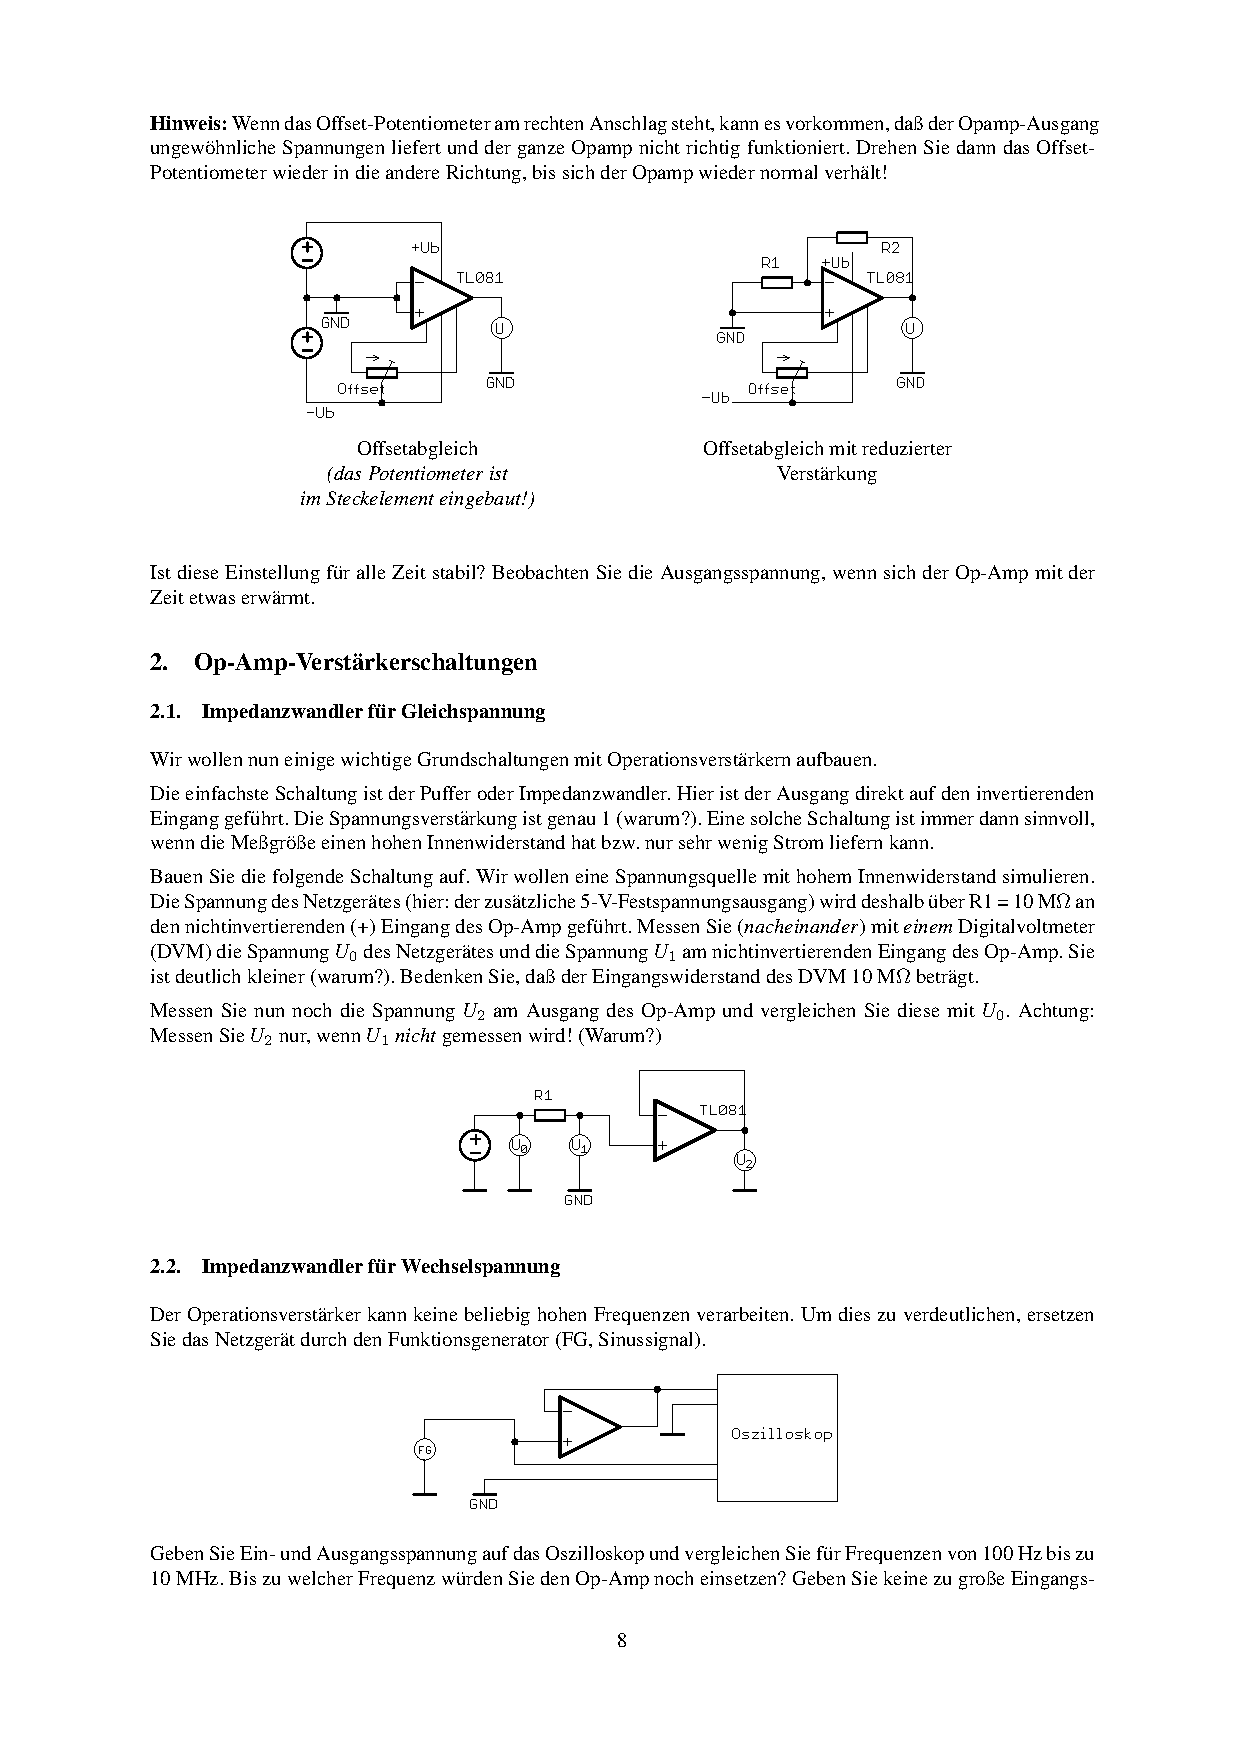
\includegraphics[trim = 10mm 90mm 10mm 180mm, clip, scale = 1]{ep4_14[Page8].pdf}
  	\caption[Schaltskizze des Impedanzwandlers für Gleichspannung]{Schaltskizze des Impedanzwandlers für Gleichspannung\footnotemark}
  \label{fig:1}
\end{figure}
\footnotetext{Abbildung entnommen von http://www.atlas.uni-wuppertal.de/$\sim$kind/ep4\_14.pdf Seite 8 am 17.11.2014}

\subsection{Versuchsdurchführung}
%erklären, !was! wir machen, !warum! wir das machen und mit welchem ziel
%(wichtig) präzize erklären, wie bei dem versuch vorgegangen und was gemacht wurde
In diesem Versuchsteil soll eine Spannung mit hohem Innenwiderstand simuliert werden. Über den Impedanzwandler kann daraus eine Spannungsquelle mit ca. \unit[100]{$\Omega$} erzeugt werden. Um diesen Effekt zu messen werden die Spannung U$_1$, U$_0$ und U$_2$ nacheinander mit dem DMM abgegriffen. Zu beachten ist der Innenwiderstand des DMMs von \unit[1]{M$\Omega$}, welcher nur $\frac{1}{10}$ des Vorwiderstandes beträgt. Dadurch entsteht also ein Spannungsteiler von $\frac{1}{11}$, für den Fall das U$_1$ gemessen wird.
\subsection{Auswertung}
%zuerst !alle! errechneten werte entweder in ganzen sätzen aufzählen, oder in tabellen (übersichtlicher) dargestellen, sowie auf die verwendeten formeln verweisen (die referenzierung der formel kann in der überschrift stehen)
%kurz erwähnen (vor der tabelle), warum wir das ganze ausrechnen bzw. was wir dort ausrechnen
%danach histogramme und plots erstellen, wobei wenn möglich funktionen durch die plots gelegt werden (zur not können auch splines benutzt werden, was aber angegeben werden muss)
%bei fits immer die funktion und das reduzierte chiquadrat mit angegeben, wobei auf verständlichkeit beim entziffern der zehnerpotenzen geachtet werden muss z.b. f(x)=(wert+-fehler)\cdot10^{irgendeine zahl}\cdot x + (wert+-fehler)\cdot10^{irgendeine zahl}
%bei jedem fit erklären, nach welchem zusammenhang gefittet wurde und warum!
%bei plots darauf achten, dass die achsenbeschriftung (auch die tics) die richtige größe haben und die legende im plot nicht die messwerte verdeckt
%kurz die aufgabenstellung abhandeln
%2-----------------------------------------------2

Am Eingang wurde U0 mit 4,99$\pm$0,06 V gemessen, U2 wurde mit 4,99$\pm$0,06 V gemessen, also ist die Ausgangsspannung genau so groß wie die Eingangsspannung. U1 wurde mit 0,45$\pm$0,06 V gemessen, dies kommt daher, das der Widerstand ein Netzgerät mit hohem Innenwiderstand simuliert.

\subsection{Diskussion}
%(immer) die gemessenen werte und die bestimmten werte über die messfehler mit literaturwerten oder untereinander vergleichen
%in welchem fehlerintervall des messwertes liegt der literaturwert oder der vergleichswert?
%wie ist der relative anteil des fehlers am messwert und damit die qualität unserer messung?
%in einem satz erklären, wie gut unser fehler und damit unsere messung ist
%kurz erläutern, wie systematische fehler unsere messung beeinflusst haben könnten
%(wichtig) zum schluss ansprechen, in wie weit die ergebnisse mit der theoretischen vorhersage übereinstimmen
%--------------------------------------------------------------------------------------------
%falls tabellen mit den messwerten zu lang werden, kann die section mit den messwerten auch hinter der diskussion angefügt bzw. eine section mit dem anhang eingefügt werden.
%1-----------------------------------------------1

Wie erwartet wurde lässt sich der Op-Amp sehr gut dazu nutzen, aus einer Spannungsquelle mit hohem Innenwiederstand in eine Spannungsquelle mit geringem Innenwiederstand umzuwandeln.

\section{Impedanzwandler für Wechselspannung}
%kurz das ziel dieses versuchsteiles ansprechen, damit keine zwei überschriften direkt übereinander stehen!
%bei schwierigeren versuchen kann auch der theoretische hintergrund erläutert werden. (mit formeln, herleitungen und erklärungen)
Der Op-Amp kann keine beliebig hohen Frequenzen verarbeiten. Das Frequenzverhalten soll am Oszilloskop untersucht werden.
\subsection{Verwendete Materialien}
%(immer) eine skizze oder ein foto einfügen, die geräte/materialien !nummerieren! und z.b. eine legende dazu schreiben, besser wäre es das ganze in einem Fließtext gut zu beschreiben.
%falls am anfang des versuches nicht klar ist, was alles verwendet wird, wenn möglich erst am ende ein großes foto von den verwendeten materialien machen!\\

Verwendet werden ein Funktionsgenerator als Spannungsquelle, ein Operationsverstärker und ein Oszilloskop zur Signaldarstellung.


\subsection{Versuchsaufbau}
%skizze zum versuchsaufbau (oder foto) einfügen,   es muss erklärt werden wie das ganze funktioniert und welche speziellen einstellungen verwendet wurden (z.b. welche knöpfe an den geräten für die messung verdreht wurden)

FG ist der Funktionsgenerator.

\begin{figure}[H] 
  \centering
    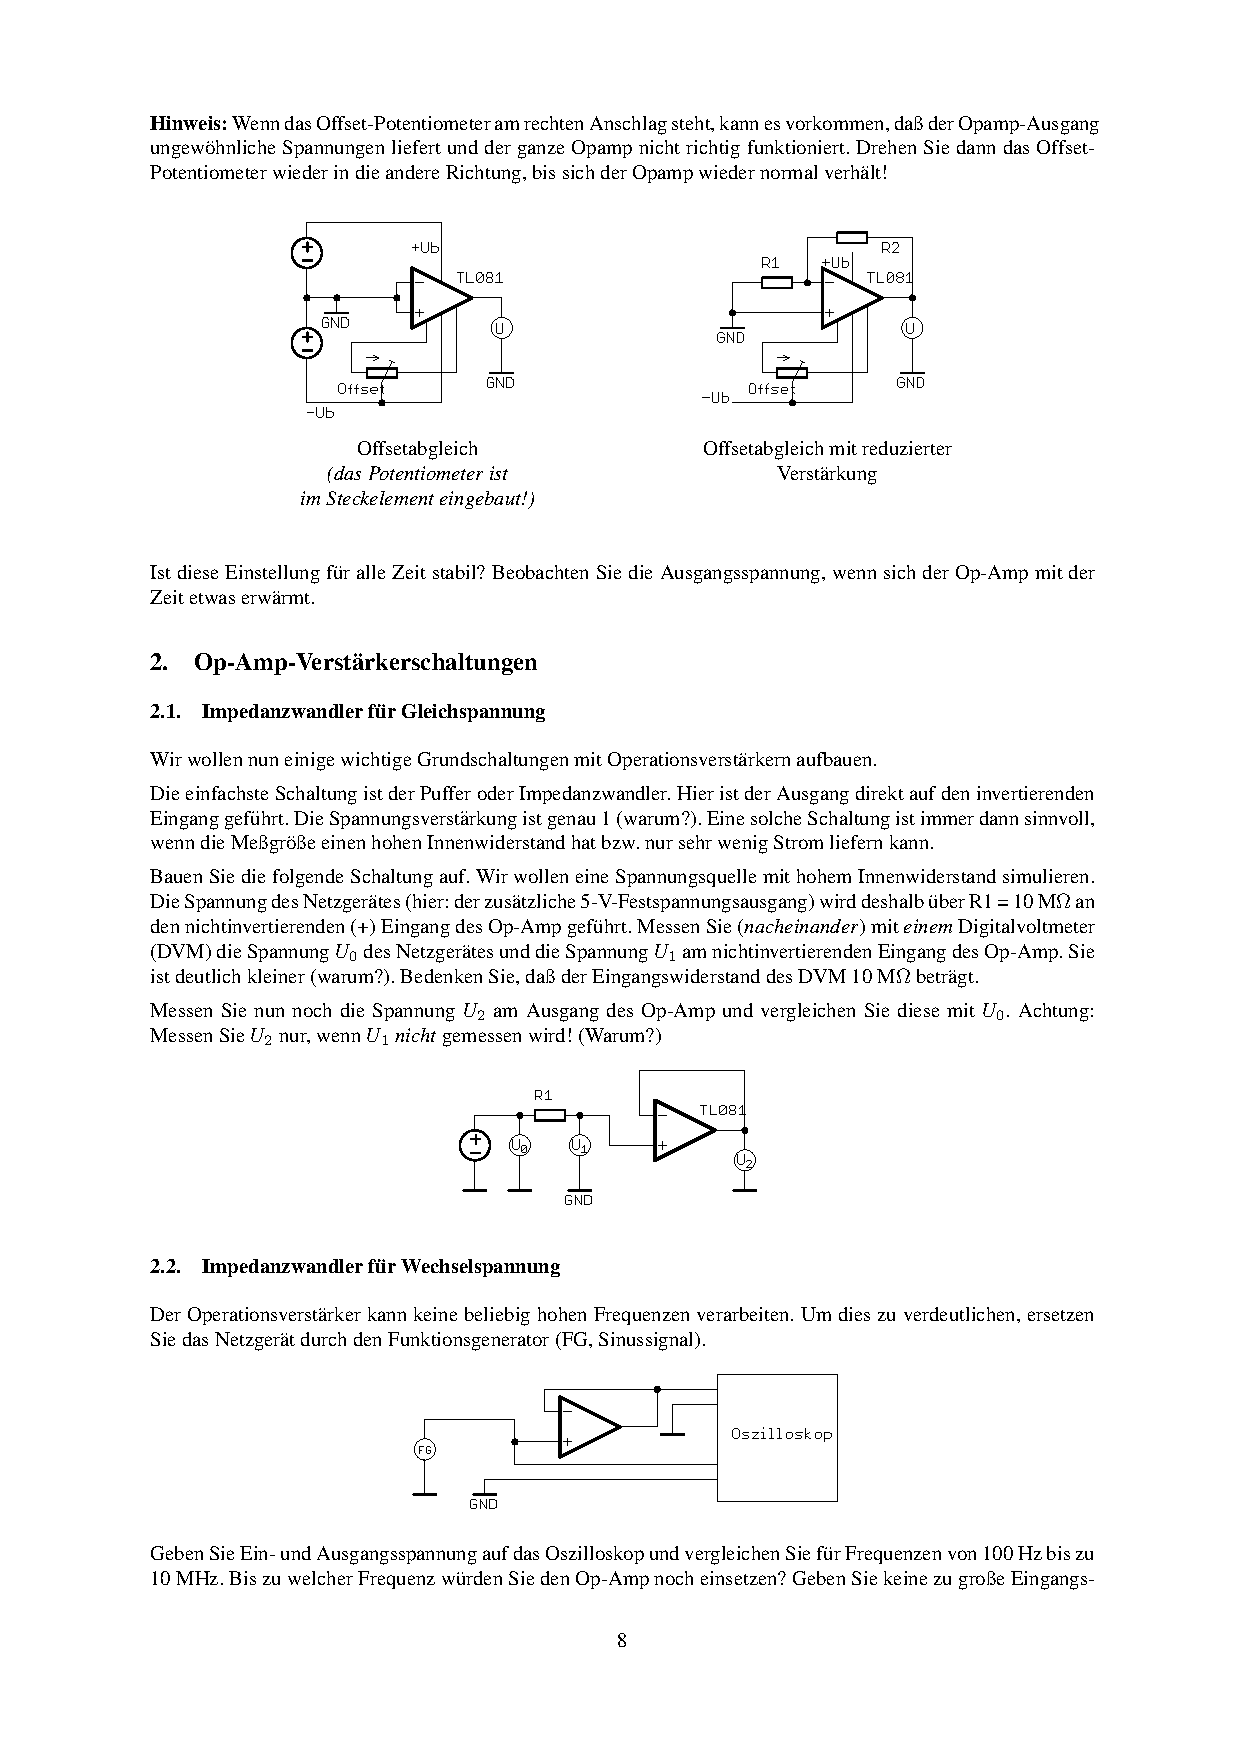
\includegraphics[trim = 10mm 40mm 10mm 230mm, clip, scale = 1]{ep4_14[Page8].pdf}
  	\caption[Schaltskizze des Impedanzwandlers für Wechselspannung]{Schaltskizze des Impedanzwandlers für Wechselspannung\footnotemark}
  \label{fig:1}
\end{figure}
\footnotetext{Abbildung entnommen von http://www.atlas.uni-wuppertal.de/$\sim$kind/ep4\_14.pdf Seite 8 am 17.11.2014}

\subsection{Versuchsdurchführung}
%erklären, !was! wir machen, !warum! wir das machen und mit welchem ziel
%(wichtig) präzize erklären, wie bei dem versuch vorgegangen und was gemacht wurde
Das Netzgerät wird durch den Funktionengenerator (Sinussignal) ersetzt, um das Verhalten des Op-Amps bei verschiedenen Frequenzen zu untersuchen. Von \unit[100]{Hz} bis \unit[10]{MHz} wird das Ausgangs und Eingangssignal miteinander verglichen.

\subsection{Auswertung}
%zuerst !alle! errechneten werte entweder in ganzen sätzen aufzählen, oder in tabellen (übersichtlicher) dargestellen, sowie auf die verwendeten formeln verweisen (die referenzierung der formel kann in der überschrift stehen)
%kurz erwähnen (vor der tabelle), warum wir das ganze ausrechnen bzw. was wir dort ausrechnen
%danach histogramme und plots erstellen, wobei wenn möglich funktionen durch die plots gelegt werden (zur not können auch splines benutzt werden, was aber angegeben werden muss)
%bei fits immer die funktion und das reduzierte chiquadrat mit angegeben, wobei auf verständlichkeit beim entziffern der zehnerpotenzen geachtet werden muss z.b. f(x)=(wert+-fehler)\cdot10^{irgendeine zahl}\cdot x + (wert+-fehler)\cdot10^{irgendeine zahl}
%bei jedem fit erklären, nach welchem zusammenhang gefittet wurde und warum!
%bei plots darauf achten, dass die achsenbeschriftung (auch die tics) die richtige größe haben und die legende im plot nicht die messwerte verdeckt
%kurz die aufgabenstellung abhandeln
%2-----------------------------------------------2


Es sollte die Eigenschaft des Op-Amp als Impedanzwandler für Wechselspannung untersucht werden, dafür wurden Eingangs- und Ausgangssignal für einen Bereich von 100 Hz bis 10 MHz aufgenommen und verglichen. Die aufgenommenen Kurven sind in Abbildung \ref{fig:2_2_a} und \ref{fig:2_2_b} zu sehen. Im Frequenzbereich von 100 Hz bis 1 MHz ist das Signal noch gut erhalten. Die erste Verzerrung tritt ab einer Frequenz von 4 MHz auf, siehe Abbildung \ref{fig:2_2_4m}.

\begin{figure}[H]
        \centering
        \begin{subfigure}[b]{0.28\textwidth}
                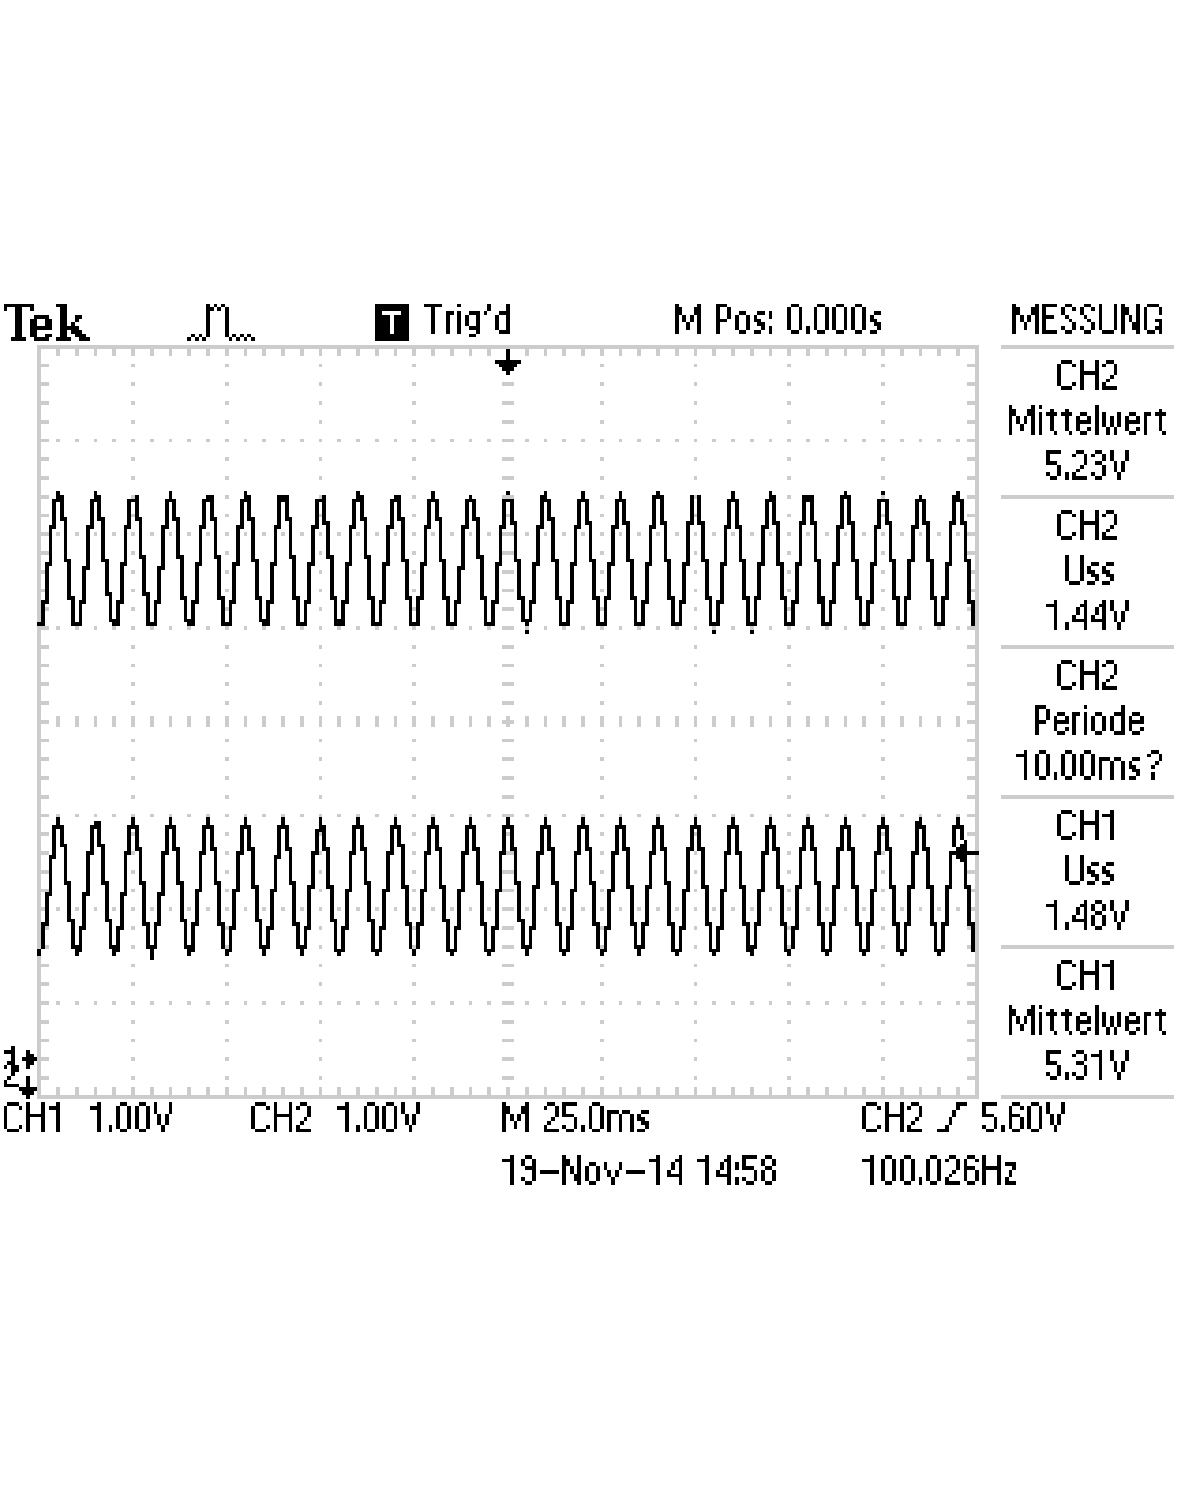
\includegraphics[width=\textwidth , scale = 0.4]{2_2_100.pdf}
                \caption[Aufnahme des Signals bei 100Hz]{Aufnahme des Signals bei 100Hz}
                \label{fig:2_2_100}
        \end{subfigure}%
       % ~ %add desired spacing between images, e. g. ~, \quad, \qquad, \hfill etc.
          %(or a blank line to force the subfigure onto a new line)
        \hfill
        \begin{subfigure}[b]{0.28\textwidth}
                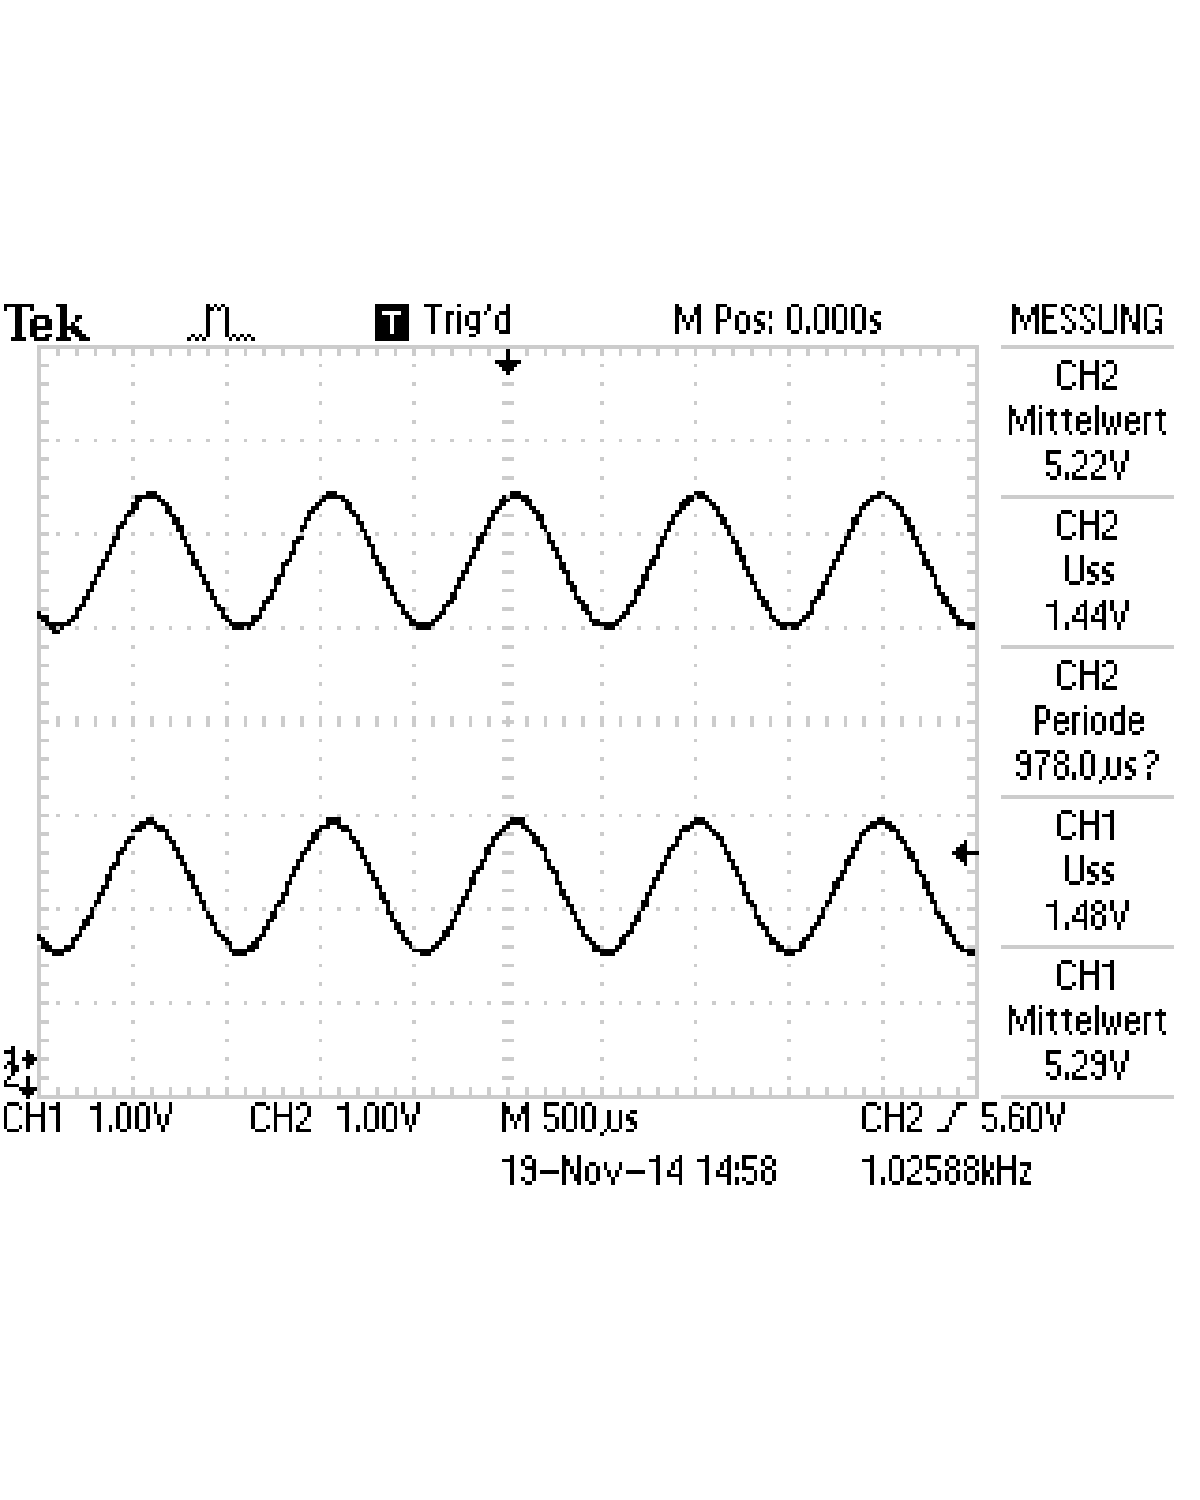
\includegraphics[width=\textwidth , scale = 0.4]{2_2_1k.pdf}
                \caption[Aufnahme des Signals bei 1kHz]{Aufnahme des Signals bei 1kHz}
                \label{fig:2_2_1k}
        \end{subfigure}
       % ~ %add desired spacing between images, e. g. ~, \quad, \qquad, \hfill etc.
          %(or a blank line to force the subfigure onto a new line)
        \hfill
        \begin{subfigure}[b]{0.28\textwidth}
                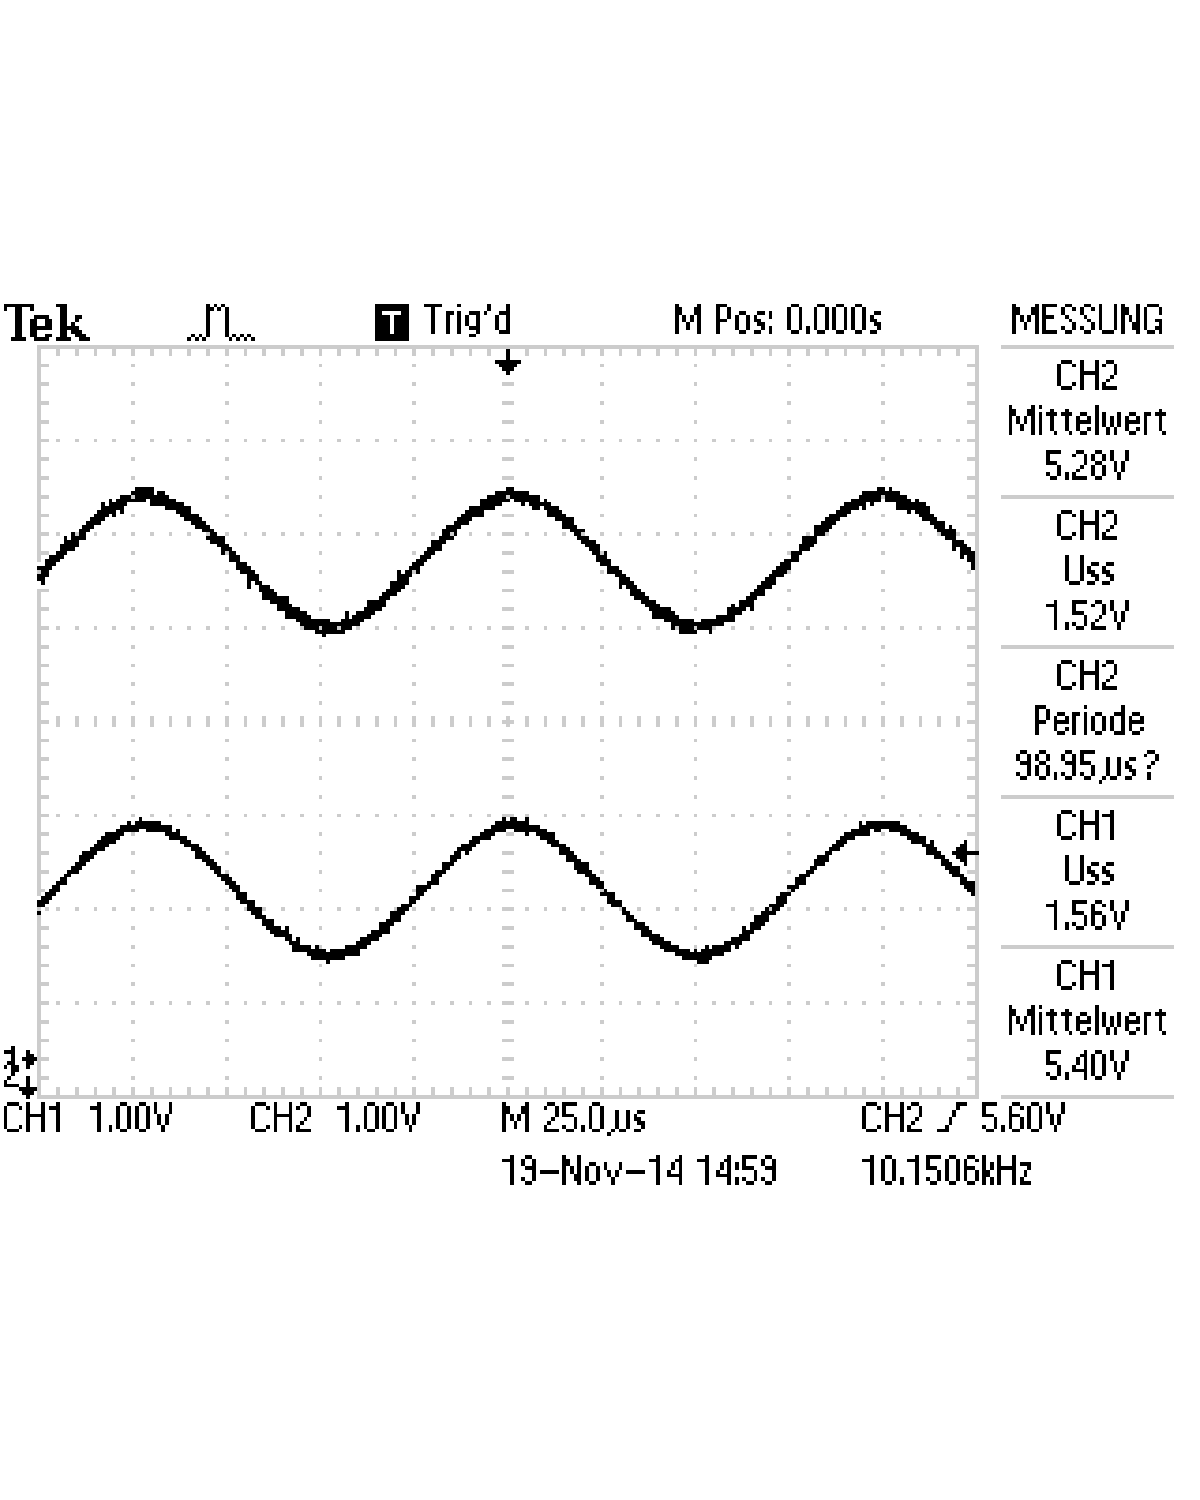
\includegraphics[width=\textwidth , scale = 0.4]{2_2_10k.pdf}
                \caption[Aufnahme des Signals bei 10kHz]{Aufnahme des Signals bei 10Hz}
  				\label{fig:2_2_10k}
        \end{subfigure}
        \caption{Kurve  für 100Hz, 1kHz und 10kHz}
        \label{fig:2_2_a}
\end{figure}

\begin{figure}[H]
        \centering
        \begin{subfigure}[b]{0.28\textwidth}
                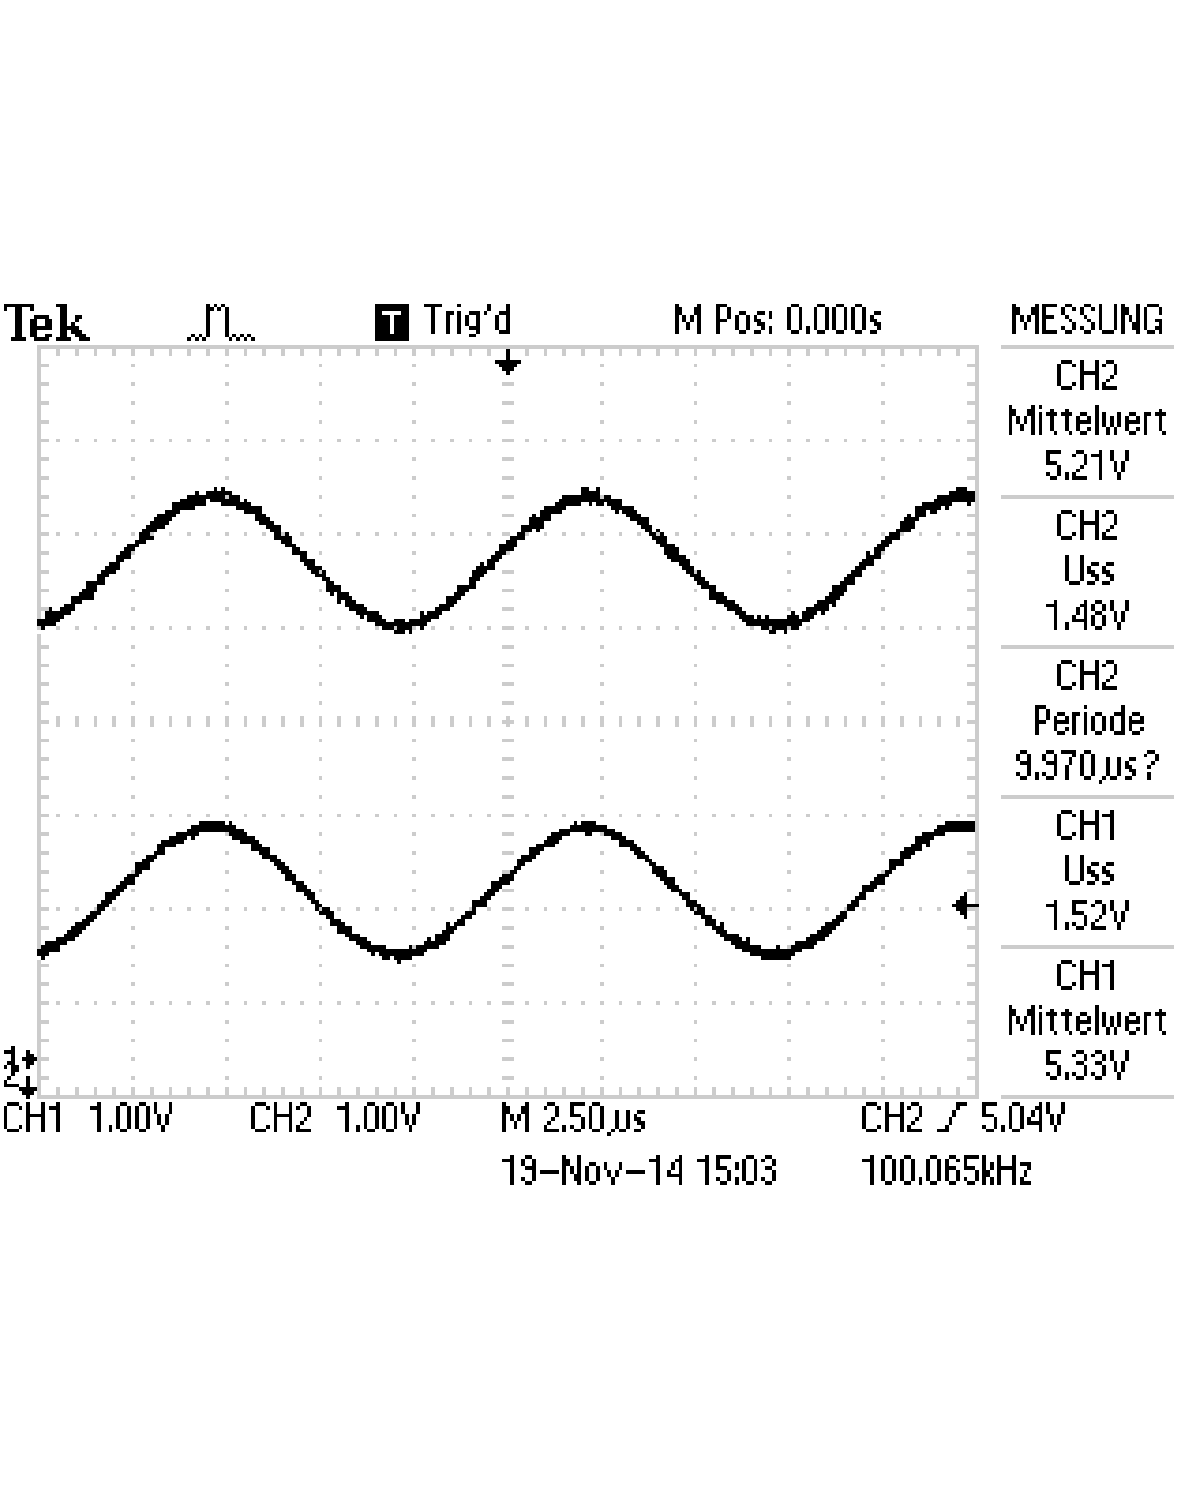
\includegraphics[width=\textwidth , scale = 0.4]{2_2_100k.pdf}
                \caption[Aufnahme des Signals bei 100kHz]{Aufnahme des Signals bei 100kHz}
                \label{fig:2_2_100k}
        \end{subfigure}%
       % ~ %add desired spacing between images, e. g. ~, \quad, \qquad, \hfill etc.
          %(or a blank line to force the subfigure onto a new line)
        \hfill
        \begin{subfigure}[b]{0.28\textwidth}
                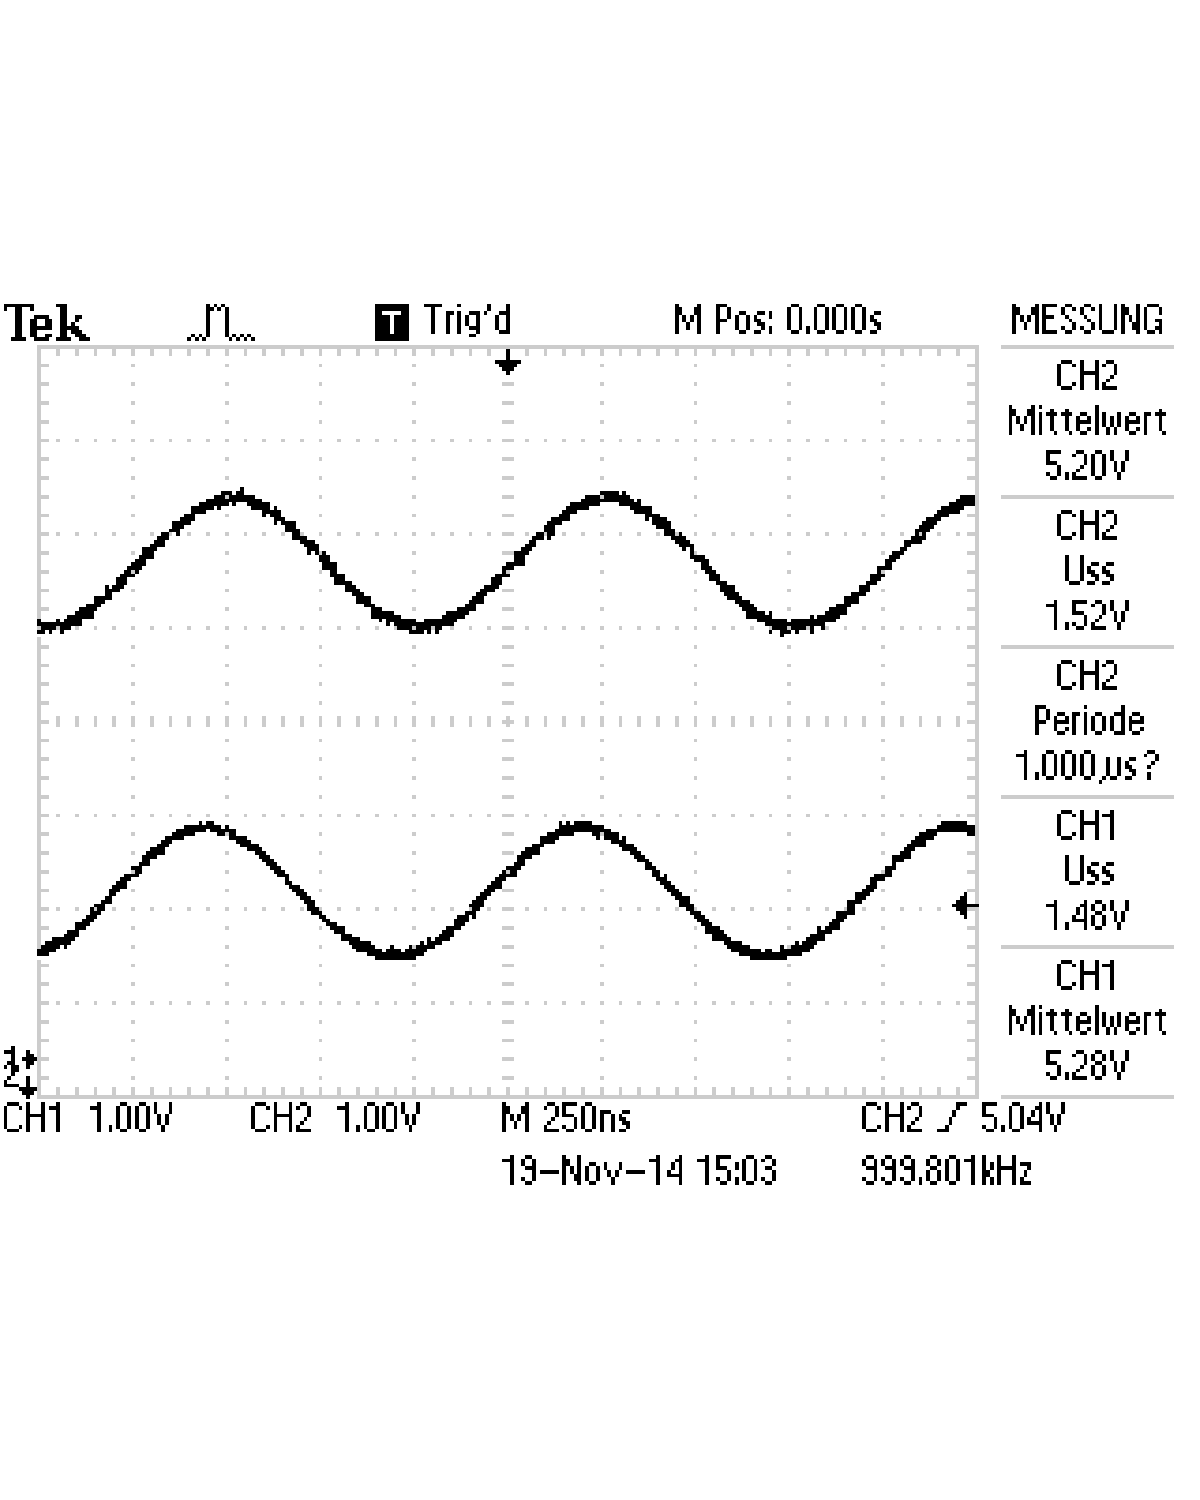
\includegraphics[width=\textwidth , scale = 0.4]{2_2_1m.pdf}
                \caption[Aufnahme des Signals bei 1mHz]{Aufnahme des Signals bei 1mHz}
                \label{fig:2_2_1m}
        \end{subfigure}
       % ~ %add desired spacing between images, e. g. ~, \quad, \qquad, \hfill etc.
          %(or a blank line to force the subfigure onto a new line)
        \hfill
        \begin{subfigure}[b]{0.28\textwidth}
                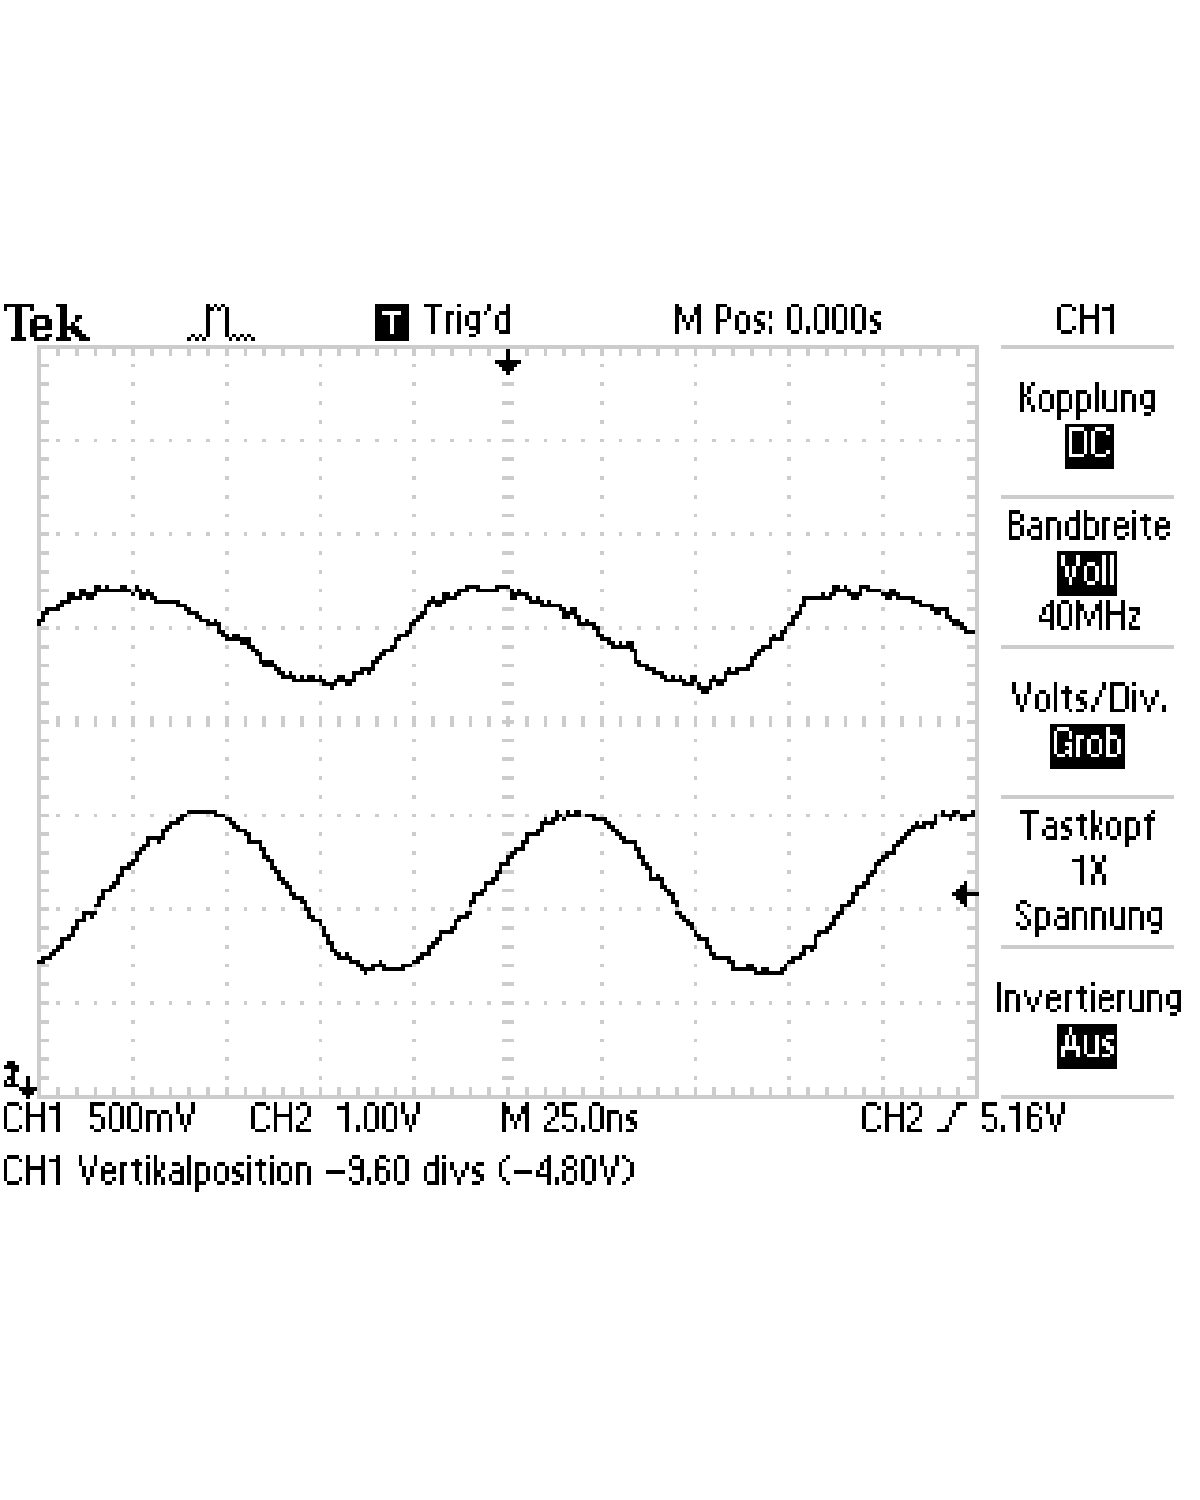
\includegraphics[width=\textwidth , scale = 0.4]{2_2_10m.pdf}
                \caption[Aufnahme des Signals bei 10mHz]{Aufnahme des Signals bei 10mHz}
  				\label{fig:2_2_10m}
        \end{subfigure}
        \caption{Kurve  für 100kHz, 1mHz und 10mHz}
        \label{fig:2_2_b}
\end{figure}

\begin{figure}[H] 
  \centering
    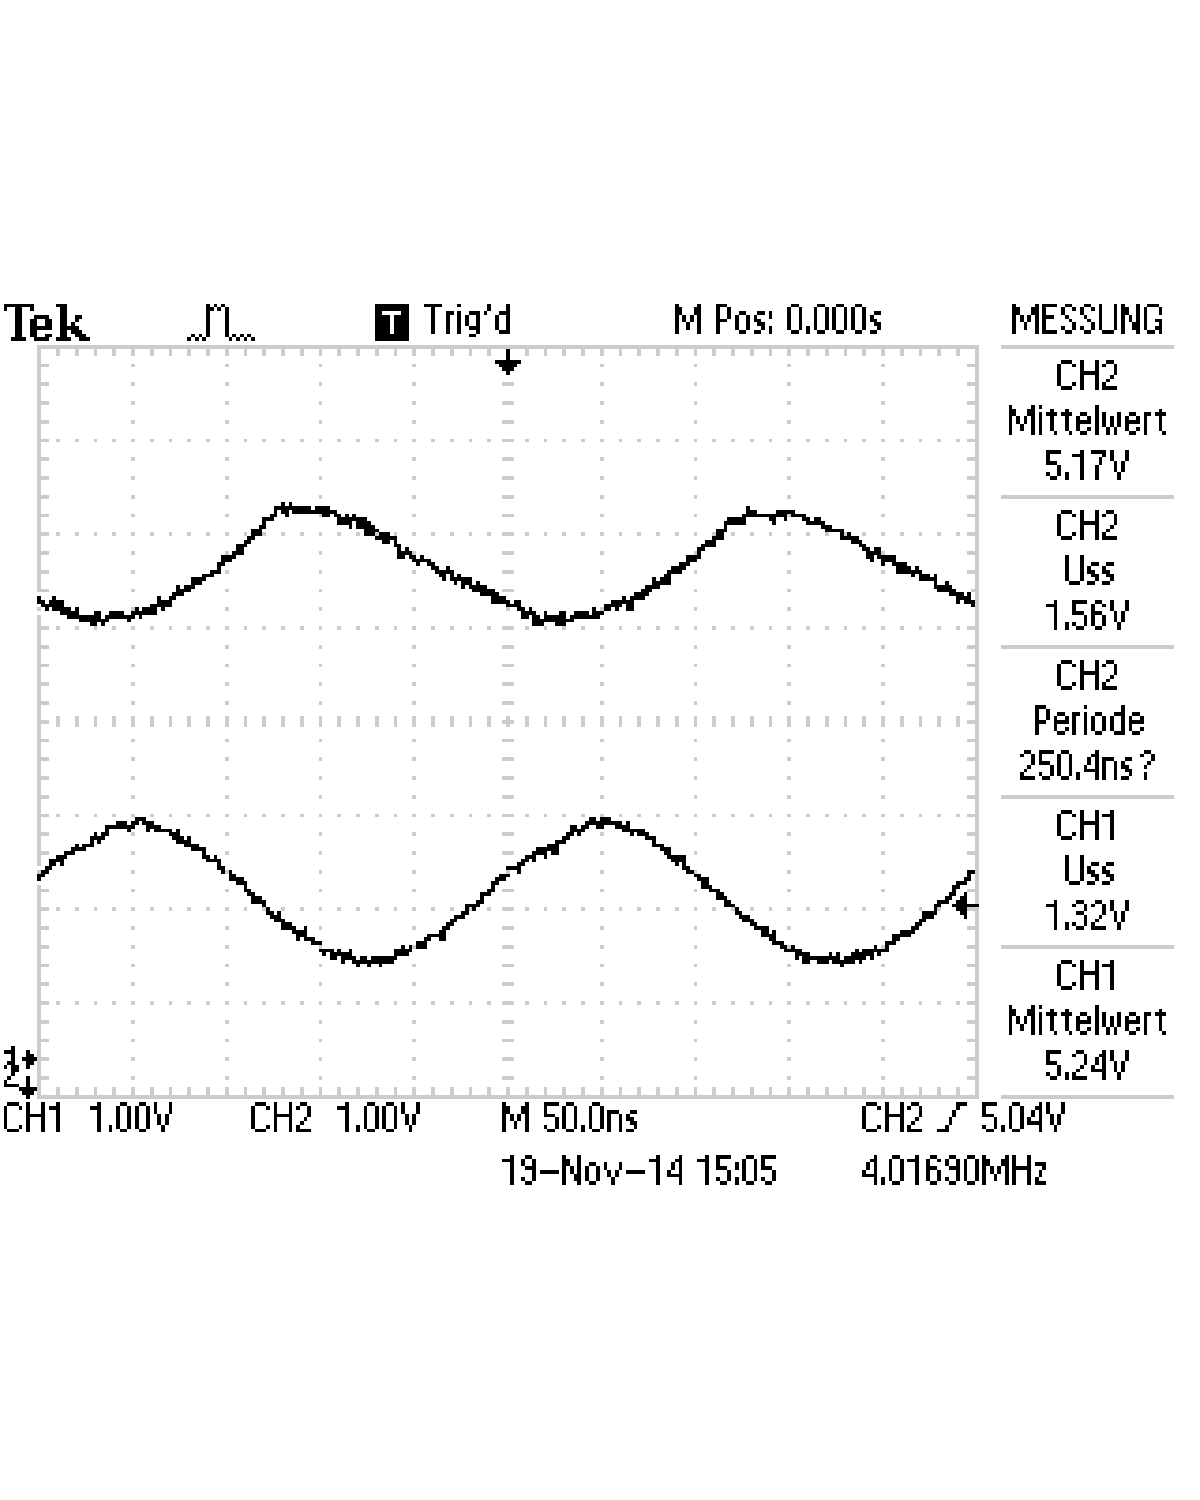
\includegraphics[ scale = 0.7]{2_2_4m.pdf}
  	\caption[Eingangs- und Ausgangsspannung für 4 MHz]{Eingangs- und Ausgangsspannung für 4 MHz}
  \label{fig:2_2_4m}
\end{figure}

\subsection{Diskussion}
%(immer) die gemessenen werte und die bestimmten werte über die messfehler mit literaturwerten oder untereinander vergleichen
%in welchem fehlerintervall des messwertes liegt der literaturwert oder der vergleichswert?
%wie ist der relative anteil des fehlers am messwert und damit die qualität unserer messung?
%in einem satz erklären, wie gut unser fehler und damit unsere messung ist
%kurz erläutern, wie systematische fehler unsere messung beeinflusst haben könnten
%(wichtig) zum schluss ansprechen, in wie weit die ergebnisse mit der theoretischen vorhersage übereinstimmen
%--------------------------------------------------------------------------------------------
%falls tabellen mit den messwerten zu lang werden, kann die section mit den messwerten auch hinter der diskussion angefügt bzw. eine section mit dem anhang eingefügt werden.
%1-----------------------------------------------1


Wie erwartet kann der Op-Amp keine beliebig hohen Frequenzen verzerrungsfrei übertragen. Ab einer Frequenz von ca. 4 MHz wird das Eingangssignal verzerrt ausgegeben.

\section{Spannungsverstärker für Wechselspannung}
%kurz das ziel dieses versuchsteiles ansprechen, damit keine zwei überschriften direkt übereinander stehen!
%bei schwierigeren versuchen kann auch der theoretische hintergrund erläutert werden. (mit formeln, herleitungen und erklärungen)
Der Op-Amp kann auch für die Spannungsverstärkung von Wechselspannungen verwendet werden.
\subsection{Verwendete Materialien}
%(immer) eine skizze oder ein foto einfügen, die geräte/materialien !nummerieren! und z.b. eine legende dazu schreiben, besser wäre es das ganze in einem Fließtext gut zu beschreiben.
%falls am anfang des versuches nicht klar ist, was alles verwendet wird, wenn möglich erst am ende ein großes foto von den verwendeten materialien machen!\\

Verwendet werden ein Funktionsgenerator, zwei Widerstände(1 und 100 k$\Omega$), ein Operationsverstärker und DVMs zur Messung.

\subsection{Verwendete Formeln}
%eine legende kann angefertigt werden, die selbstverständlichen buchstaben müssen nicht extra erklärt werden
%mit knappen erklärungen die !verwendeten! formeln, sowie die zugehörige fehlerrechnung einfügen
%2-----------------------------------------------2
Aus dem Verhältnis der Widerstände ergibt sich bei einem Idealen Op-Amp die Spannungsverstärkung nach:
\begin{align}
U_2 = -\frac{R2}{R1}U_1
\end{align}
%ab hier kann nochmal in einzelne versuchsteile unterteilt werden
\subsection{Versuchsaufbau}
%skizze zum versuchsaufbau (oder foto) einfügen,   es muss erklärt werden wie das ganze funktioniert und welche speziellen einstellungen verwendet wurden (z.b. welche knöpfe an den geräten für die messung verdreht wurden)

FG ist der Funktionsgenerator, R1 ist ein 1k$\Omega$ Widerstand und R2 ein 100k$\Omega$ Widerstand.

\begin{figure}[H] 
  \centering
    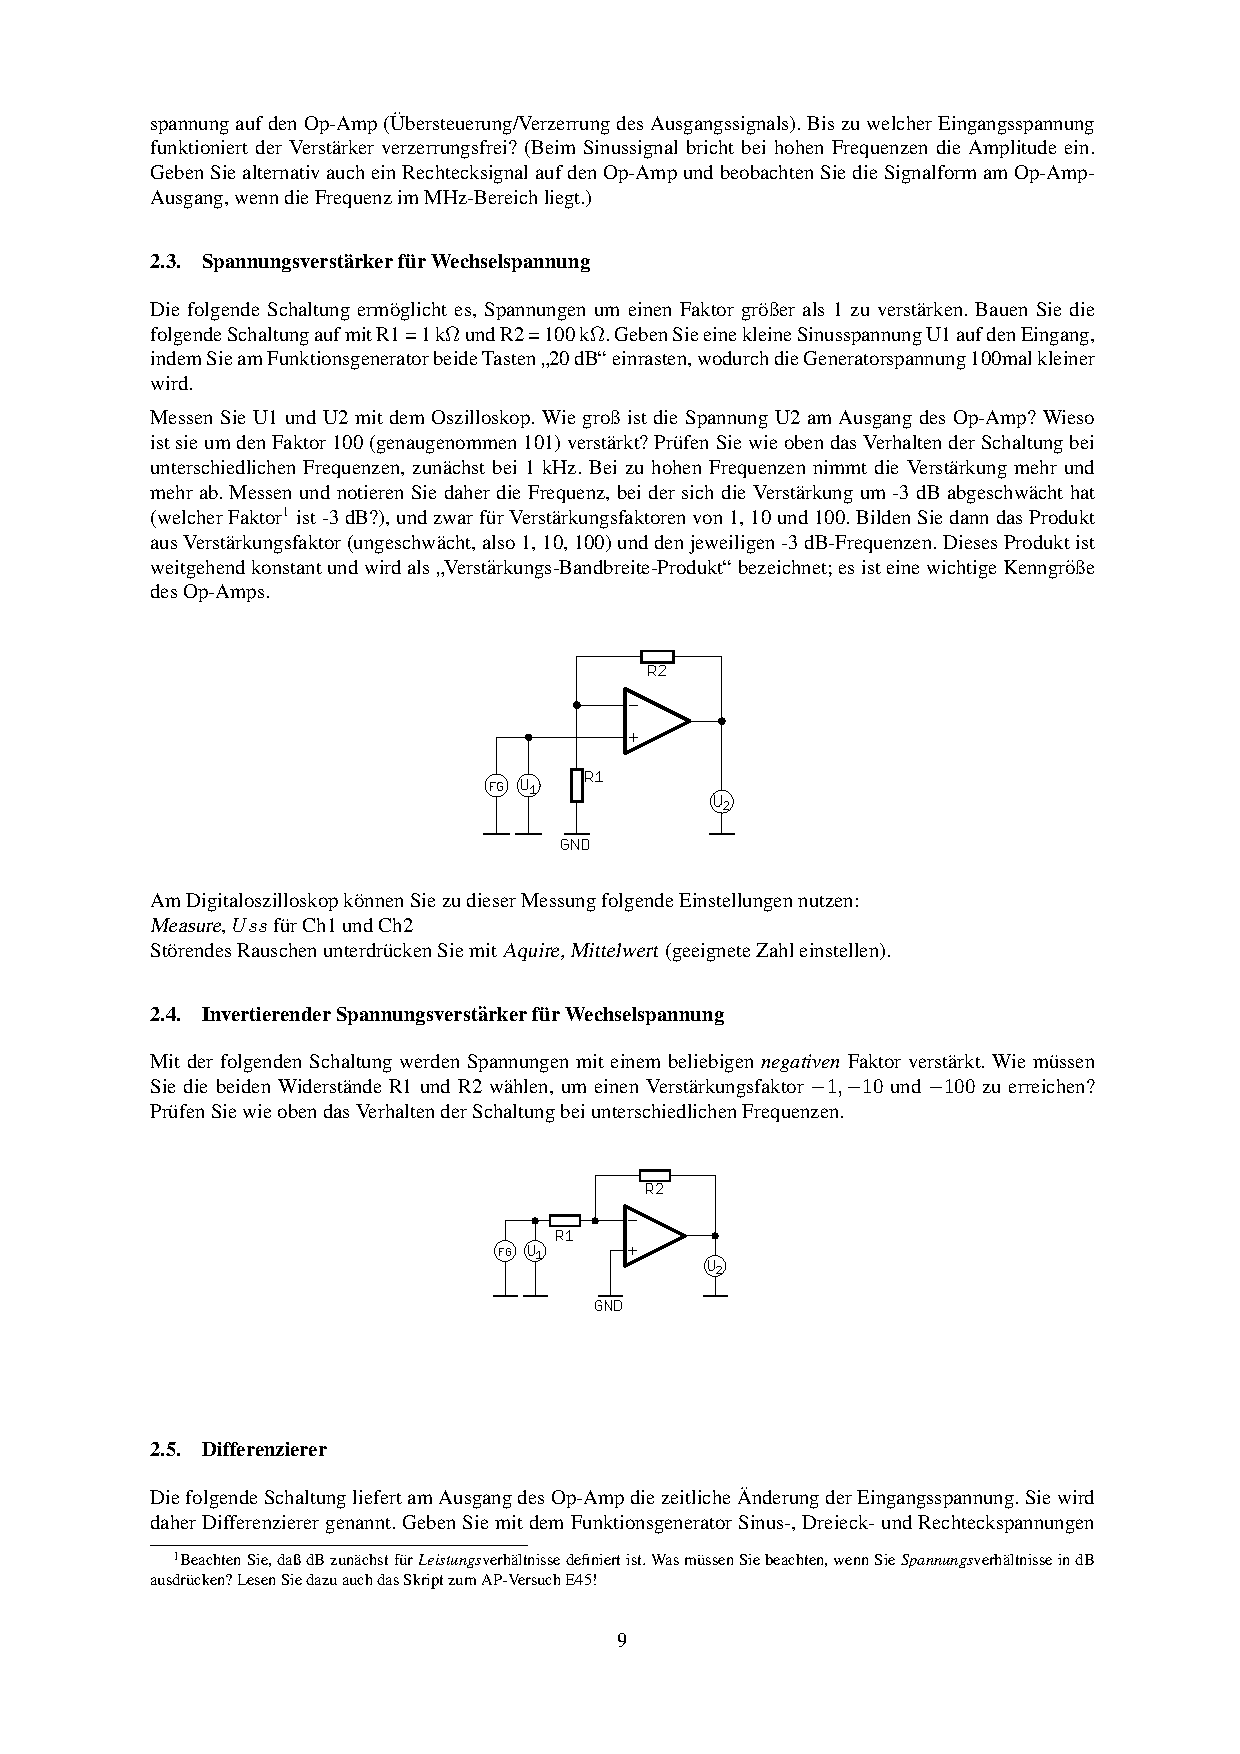
\includegraphics[trim = 10mm 70mm 10mm 195mm, clip, scale = 1]{ep4_14[Page9].pdf}
  	\caption[Schaltskizze des Spannungsverstärkers für Wechselspannung]{Schaltskizze des Spannungsverstärkers für Wechselspannung\footnotemark}
  \label{fig:1}
\end{figure}
\footnotetext{Abbildung entnommen von http://www.atlas.uni-wuppertal.de/$\sim$kind/ep4\_14.pdf Seite 9 am 17.11.2014}

\subsection{Versuchsdurchführung}
%erklären, !was! wir machen, !warum! wir das machen und mit welchem ziel
%(wichtig) präzize erklären, wie bei dem versuch vorgegangen und was gemacht wurde
In diesem Versuchsteil wird der Op-Amp für eine Spannungsverstärkerschaltung von Wechselspannungen verwendet. Der gemessene Varstärkungsfaktor kann mit dem Verhältnis der Widerstände verglichen werden. Bei den Frequenzen, bei denen der Verstärkungsfaktor bei 1, 10 und 100 liegt, wird die Frequenz hochgedreht, bis der Verstärkungsfaktor auf $\frac{1}{\sqrt{2}}$ abgefallen ist, um das sogenannte 'Verstärkungs-Bandbreite-Produkt' auszurechnen. Dies ist eine wichtige Kenngröße des Op-Amps, welche über das Produkt von der zweiten Frequenz mit dem Verstärkungsfaktor (1,10 und 100) bestimmt werden kann. Nach dem Datenblatt\footnote{ Datenblatt Texas Instruments https://cdn-reichelt.de/documents/datenblatt/A200/TL081\_TL082\_TL084\%23TEX.pdf  } ist ein Wert im Bereich von \unitfrac[3000]{1}{s} zu erwarten, unser Wert wurde bei einem anderem Aufbau gemessen und sollte nur in der selben Größenordung liegen.
\subsection{Messergebnisse}
%die messwerte in !übersichtlichen! tabellen angegeben
%zu viele kleine tabellen in große tabellen überführen!
%zu große tabellen mit dem [scale]-befehl scalieren oder (falls zu lang) in zwei kleinere tabellen aufteilen
%(wichtig) vor !jeder! tabelle sagen, was gemessen wurde und wie die fehler gewählt wurden und ausreichend !erklären!, !warum! wir unsere fehler grade so gewählt haben

Der Fehler der gemessenen Frequenz liegt bei 5 Hz.

\begin{table}[H]
\caption{Messwerte zur Verstäkungs-Bandbreite-Produkt}
\begin{center}
\begin{tabular}{|r|r|r|}
\hline
\multicolumn{1}{|l|}{Verstärkung} & \multicolumn{1}{l|}{-3dB Frequenz/Hz} & \multicolumn{1}{l|}{Verstärkungs-Bandbreite-Produkt} \\ \hline
100 & 24 & 2400 \\ \hline
10 & 275,7 & 2757 \\ \hline
1 & 2265 & 2265 \\ \hline
\end{tabular}
\end{center}
\label{tab:2_3}
\end{table}


\subsection{Auswertung}
%zuerst !alle! errechneten werte entweder in ganzen sätzen aufzählen, oder in tabellen (übersichtlicher) dargestellen, sowie auf die verwendeten formeln verweisen (die referenzierung der formel kann in der überschrift stehen)
%kurz erwähnen (vor der tabelle), warum wir das ganze ausrechnen bzw. was wir dort ausrechnen
%danach histogramme und plots erstellen, wobei wenn möglich funktionen durch die plots gelegt werden (zur not können auch splines benutzt werden, was aber angegeben werden muss)
%bei fits immer die funktion und das reduzierte chiquadrat mit angegeben, wobei auf verständlichkeit beim entziffern der zehnerpotenzen geachtet werden muss z.b. f(x)=(wert+-fehler)\cdot10^{irgendeine zahl}\cdot x + (wert+-fehler)\cdot10^{irgendeine zahl}
%bei jedem fit erklären, nach welchem zusammenhang gefittet wurde und warum!
%bei plots darauf achten, dass die achsenbeschriftung (auch die tics) die richtige größe haben und die legende im plot nicht die messwerte verdeckt
%kurz die aufgabenstellung abhandeln
%2-----------------------------------------------2

In diesem Versuchsteil soll die Eigenschaft des Op-Amp zur Spannungsverstärkung von Wechselspannung untersucht werden. Dafür wird die Frequenz des Eingangssignals so eingestellt, das die Verstärkung 100, 10 und 1 beträgt. Dann wird die Frequenz so lange erhöht, bis eine Abschwächung der Verstärkung -3dB beträgt. Aus den Frequenzen der um -3dB verringerten Abschwächung und dem vorherigem Verstärkungsfaktor wird durch Multiplikation der Werte das Verstärkungs-Bandbreite-Produkt berechnet, welches eine Materialeigenschaft darstellt.
Mit den Werten aus Tabelle \ref{tab:2_3} ergibt sich ein Mittelwert von 2474$\pm$208 Hz für das Verstärkungs-Bandbreite-Produkt.

\subsection{Diskussion}
%(immer) die gemessenen werte und die bestimmten werte über die messfehler mit literaturwerten oder untereinander vergleichen
%in welchem fehlerintervall des messwertes liegt der literaturwert oder der vergleichswert?
%wie ist der relative anteil des fehlers am messwert und damit die qualität unserer messung?
%in einem satz erklären, wie gut unser fehler und damit unsere messung ist
%kurz erläutern, wie systematische fehler unsere messung beeinflusst haben könnten
%(wichtig) zum schluss ansprechen, in wie weit die ergebnisse mit der theoretischen vorhersage übereinstimmen
%--------------------------------------------------------------------------------------------
%falls tabellen mit den messwerten zu lang werden, kann die section mit den messwerten auch hinter der diskussion angefügt bzw. eine section mit dem anhang eingefügt werden.
%1-----------------------------------------------1

Das gemessene Verstärkungs-Bandbreite-Produkt, welches mit 2474$\pm$208 Hz bestimmt wurde in der erwarteten Größenordnung (3000 Hz).

\section{Invertierender Spannungsverstärker für Wechselspannung}
%kurz das ziel dieses versuchsteiles ansprechen, damit keine zwei überschriften direkt übereinander stehen!
%bei schwierigeren versuchen kann auch der theoretische hintergrund erläutert werden. (mit formeln, herleitungen und erklärungen)
Mit dem Invertierenden Spannungsverstärker wird die Spannung zusätzlich invertiert.
\subsection{Verwendete Geräte}
%(immer) eine skizze oder ein foto einfügen, die geräte/materialien !nummerieren! und z.b. eine legende dazu schreiben, besser wäre es das ganze in einem Fließtext gut zu beschreiben.
%falls am anfang des versuches nicht klar ist, was alles verwendet wird, wenn möglich erst am ende ein großes foto von den verwendeten materialien machen!\\

Es werden ein Operationsverstärker, zwei Widerstände, ein Funktionsgenerator und DVMs verwendet.


\subsection{Versuchsaufbau}
%skizze zum versuchsaufbau (oder foto) einfügen,   es muss erklärt werden wie das ganze funktioniert und welche speziellen einstellungen verwendet wurden (z.b. welche knöpfe an den geräten für die messung verdreht wurden)

R1 und R2 werden jeweils so gewählt, dass eine Verstärkung von -1, -10 und -100 erreicht werden.

\begin{figure}[H] 
  \centering
    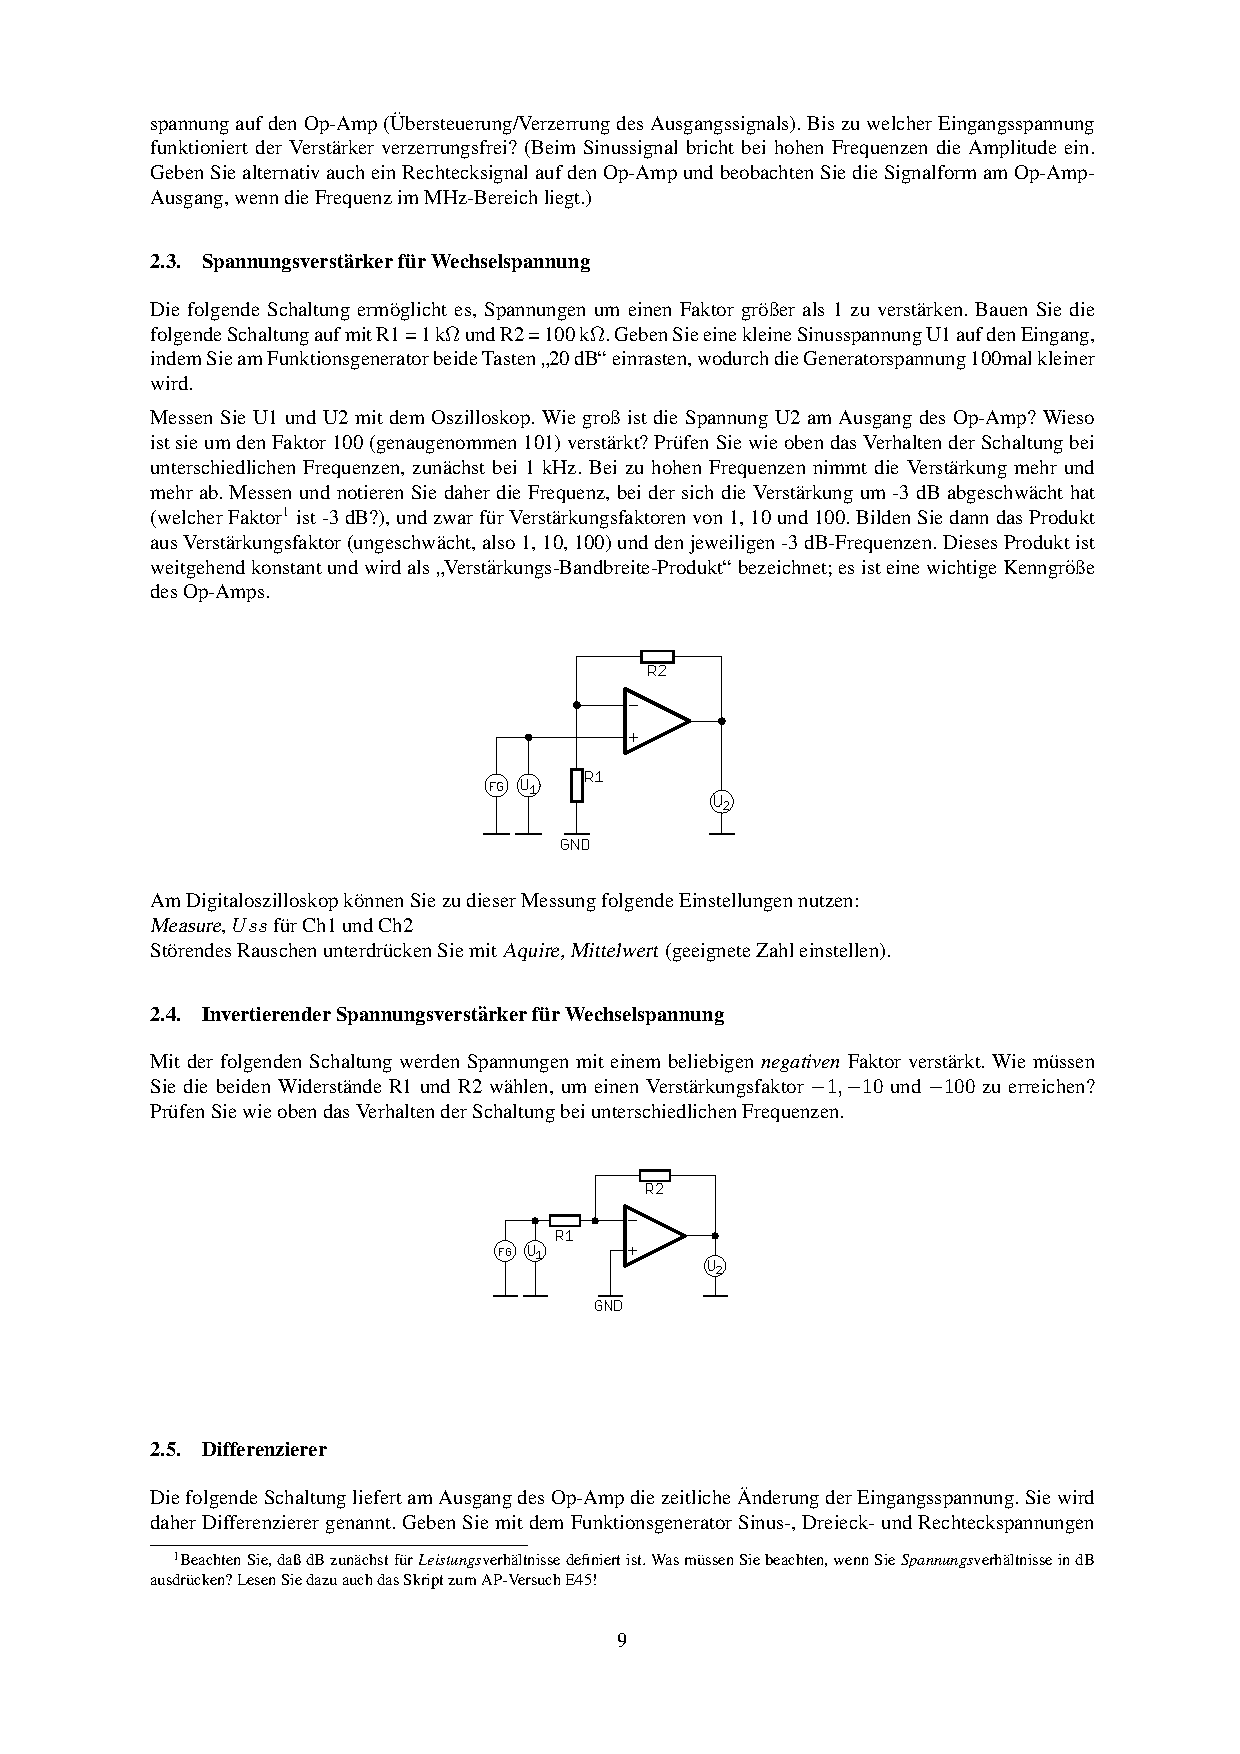
\includegraphics[trim = 10mm 65mm 10mm 195mm, clip, scale = 1]{ep4_14[Page9].pdf}
  	\caption[Schaltskizze des invertierten Spannungsverstärkers für Wechselspannung]{Schaltskizze des invertierten Spannungsverstärkers für Wechselspannung\footnotemark}
  \label{fig:1}
\end{figure}
\footnotetext{Abbildung entnommen von http://www.atlas.uni-wuppertal.de/$\sim$kind/ep4\_14.pdf Seite 9 am 17.11.2014}

\subsection{Versuchsdurchführung}
%erklären, !was! wir machen, !warum! wir das machen und mit welchem ziel
%(wichtig) präzize erklären, wie bei dem versuch vorgegangen und was gemacht wurde
Mit dem Invertierenden Spannungsverstärker für Wechselspannungen kann die Spannung nicht nur verstärkt, sondern auch invertiert werden. Das Verhalten der Schaltung wird bei Verstärkungsfaktoren von -1, -10 und -100 bei Frequenzen von \unit[1]{kHz} bis \unit[1]{MHz} beobachtet.

\subsection{Auswertung}
%zuerst !alle! errechneten werte entweder in ganzen sätzen aufzählen, oder in tabellen (übersichtlicher) dargestellen, sowie auf die verwendeten formeln verweisen (die referenzierung der formel kann in der überschrift stehen)
%kurz erwähnen (vor der tabelle), warum wir das ganze ausrechnen bzw. was wir dort ausrechnen
%danach histogramme und plots erstellen, wobei wenn möglich funktionen durch die plots gelegt werden (zur not können auch splines benutzt werden, was aber angegeben werden muss)
%bei fits immer die funktion und das reduzierte chiquadrat mit angegeben, wobei auf verständlichkeit beim entziffern der zehnerpotenzen geachtet werden muss z.b. f(x)=(wert+-fehler)\cdot10^{irgendeine zahl}\cdot x + (wert+-fehler)\cdot10^{irgendeine zahl}
%bei jedem fit erklären, nach welchem zusammenhang gefittet wurde und warum!
%bei plots darauf achten, dass die achsenbeschriftung (auch die tics) die richtige größe haben und die legende im plot nicht die messwerte verdeckt
%kurz die aufgabenstellung abhandeln
%2-----------------------------------------------2

In Versuchsteil 2.4 sollte die Eigenschaften des Op-Amp als invertierter Spannungsverstärker untersucht werden, dafür wurden Verstärkungsfaktoren von -1, -10 und -100 genommen. Die Verstärkungsfaktoren wurden durch das Verhältnis der beiden Widerstände bestimmt.
Es ist zu erkenne, dass bei hohen Frequenzen die Ausgangsspannung nicht mehr invertiert ist sonder noch eine Zusätzliche Verschiebung aufweist.


\begin{figure}[H]
        \centering
        \begin{subfigure}[b]{0.28\textwidth}
                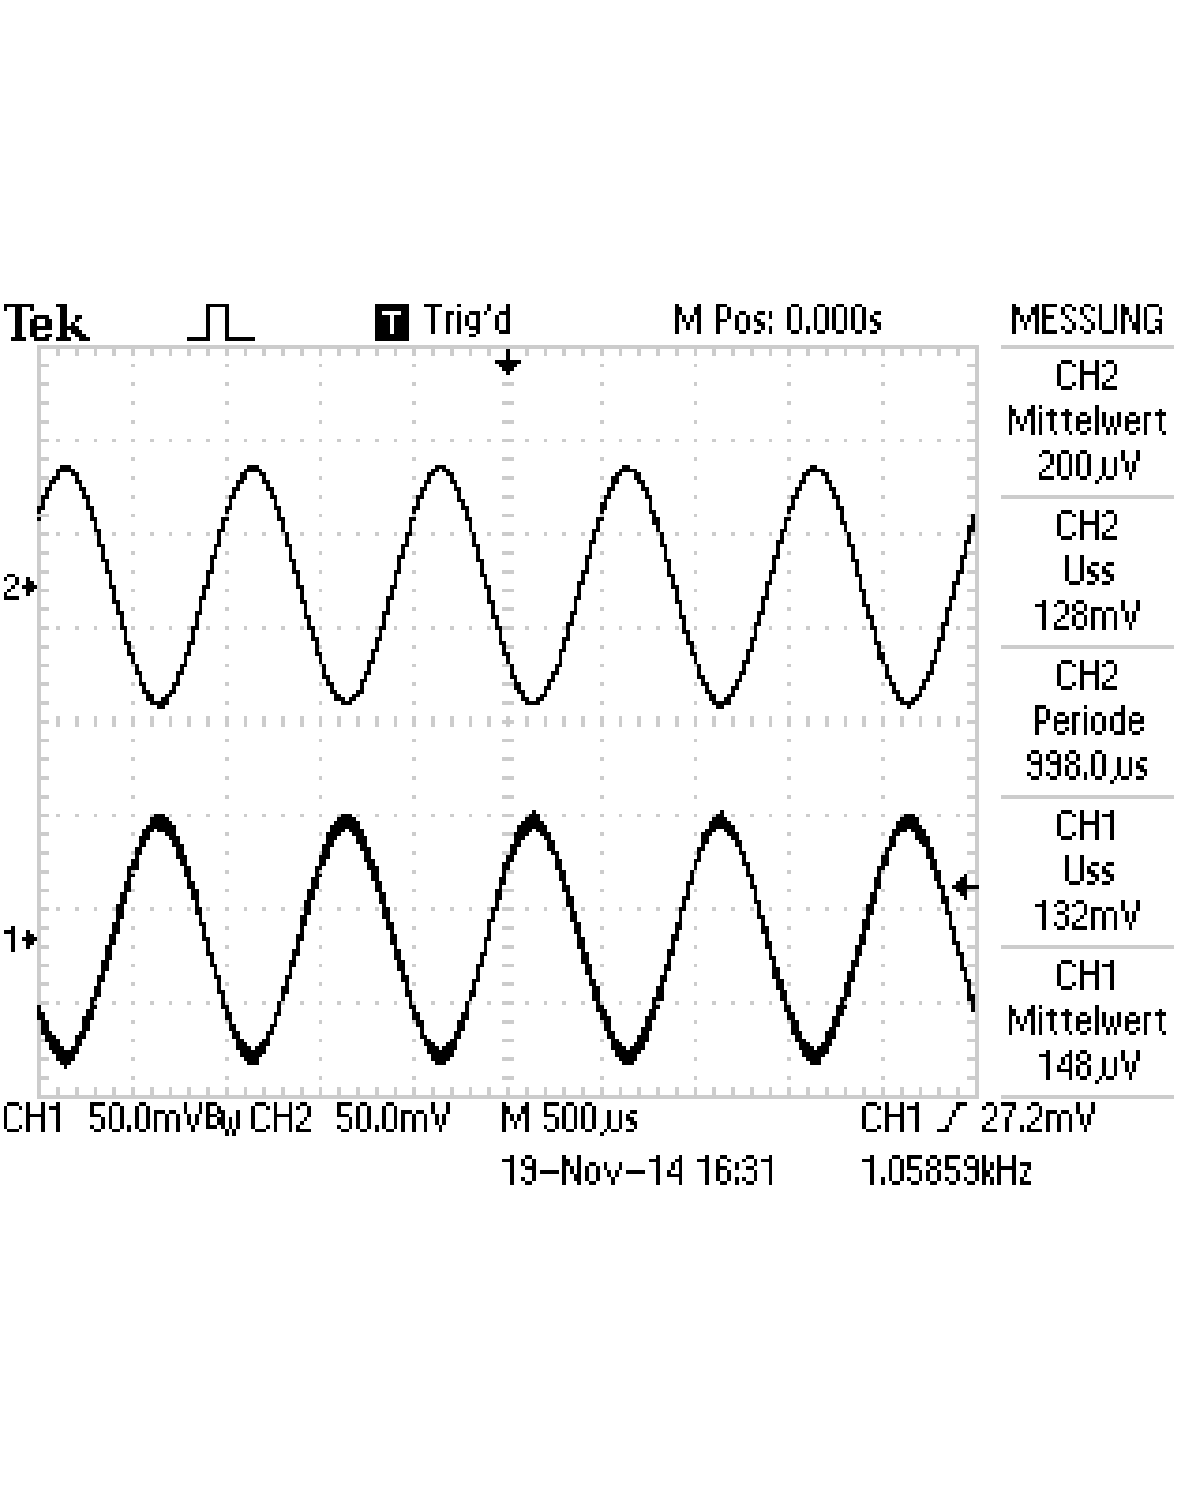
\includegraphics[width=\textwidth , scale = 0.4]{2_4_1_1k.pdf}
                \caption[Aufnahme des Signals bei 1kHz]{Aufnahme des Signals bei 1kHz}
                \label{fig:2_4_1_1k}
        \end{subfigure}%
       % ~ %add desired spacing between images, e. g. ~, \quad, \qquad, \hfill etc.
          %(or a blank line to force the subfigure onto a new line)
        \hfill
        \begin{subfigure}[b]{0.28\textwidth}
                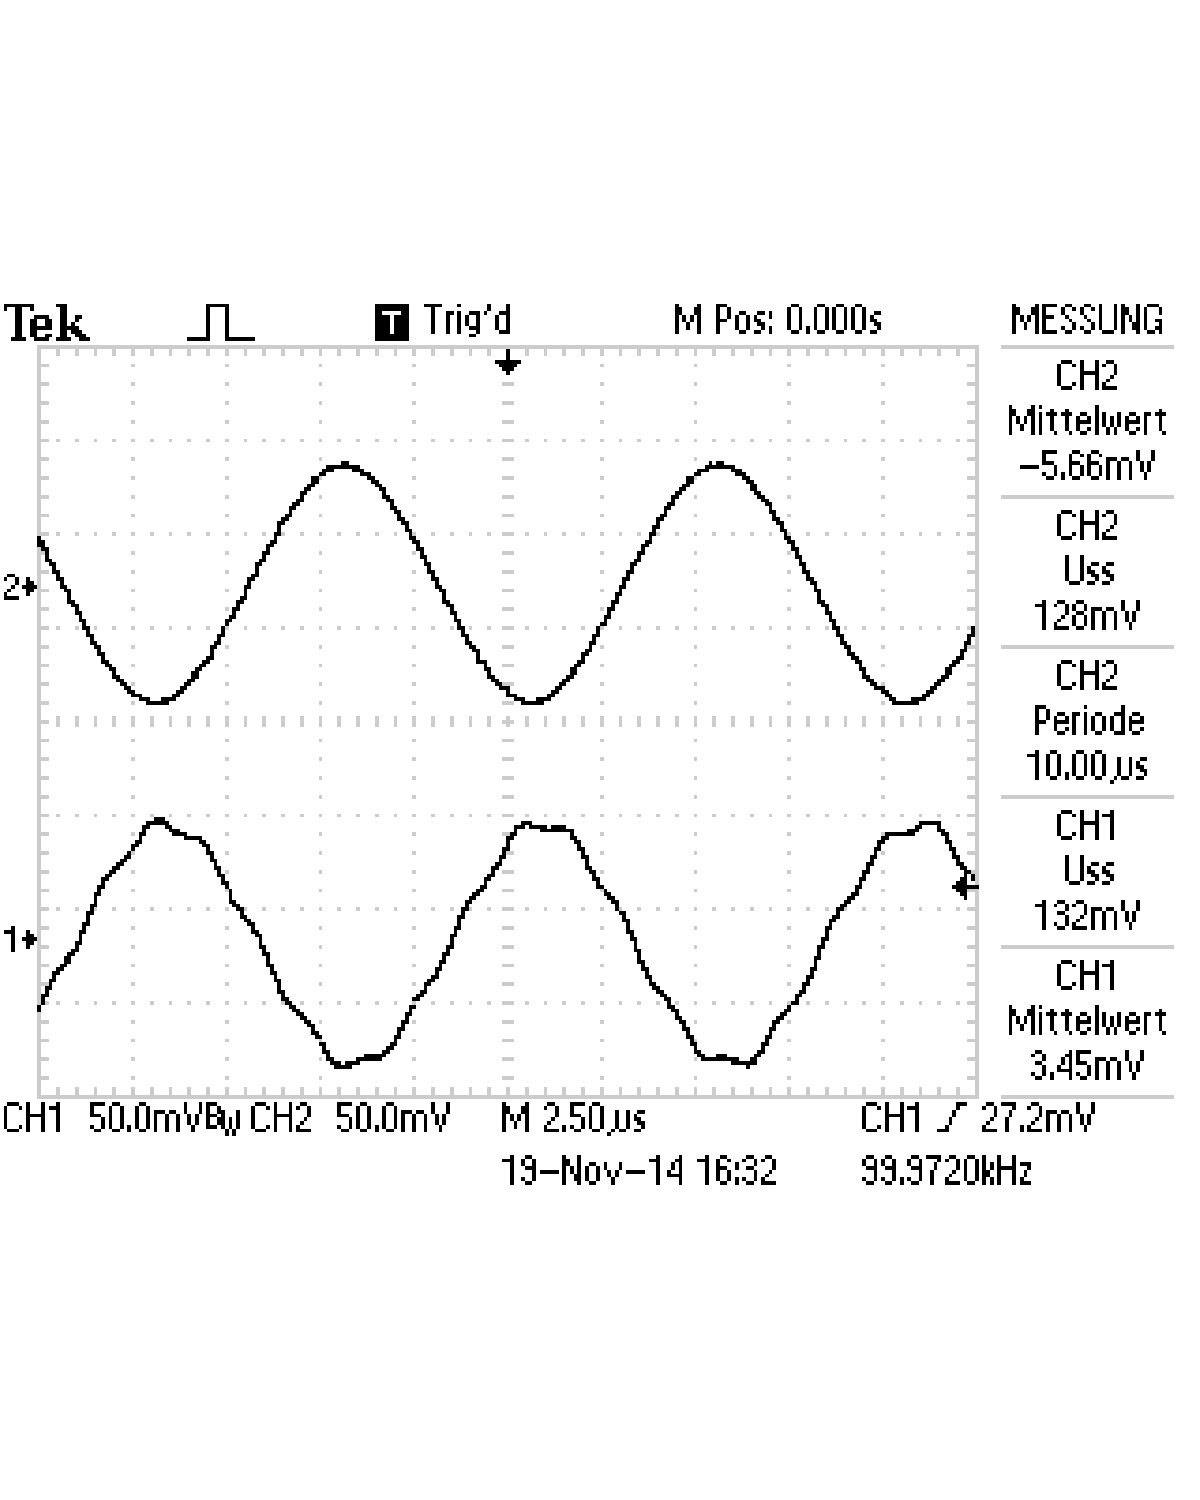
\includegraphics[width=\textwidth , scale = 0.4]{2_4_1_100k.pdf}
                \caption[Aufnahme des Signals bei 100kHz]{Aufnahme des Signals bei 100kHz}
                \label{fig:2_4_1_100k}
        \end{subfigure}
       % ~ %add desired spacing between images, e. g. ~, \quad, \qquad, \hfill etc.
          %(or a blank line to force the subfigure onto a new line)
        \hfill
        \begin{subfigure}[b]{0.28\textwidth}
                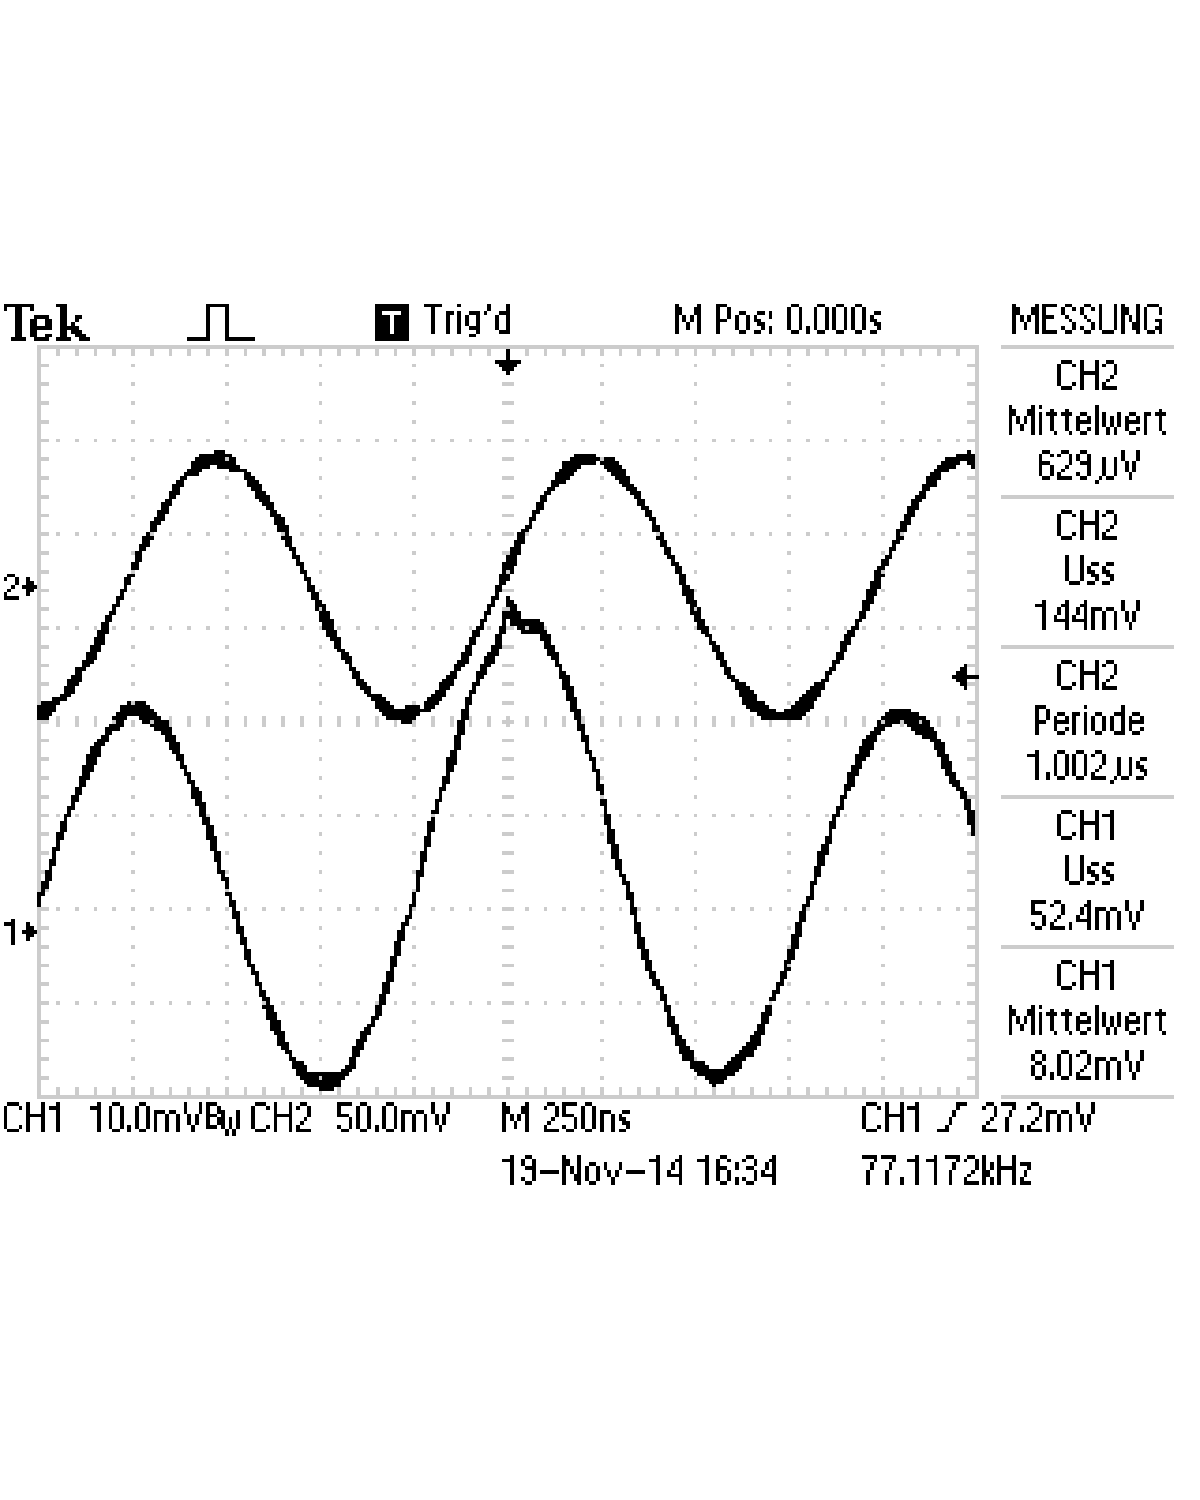
\includegraphics[width=\textwidth , scale = 0.4]{2_4_1_1m.pdf}
                \caption[Aufnahme des Signals bei 1mHz]{Aufnahme des Signals bei 1mHz}
  				\label{fig:2_4_1_1m}
        \end{subfigure}
        \caption{Kurven für 1kHz, 100kHz und 1mHz, bei einer Verstärkung von -1}
        \label{fig:2_4_1}
\end{figure}


\begin{figure}[H]
        \centering
        \begin{subfigure}[b]{0.28\textwidth}
                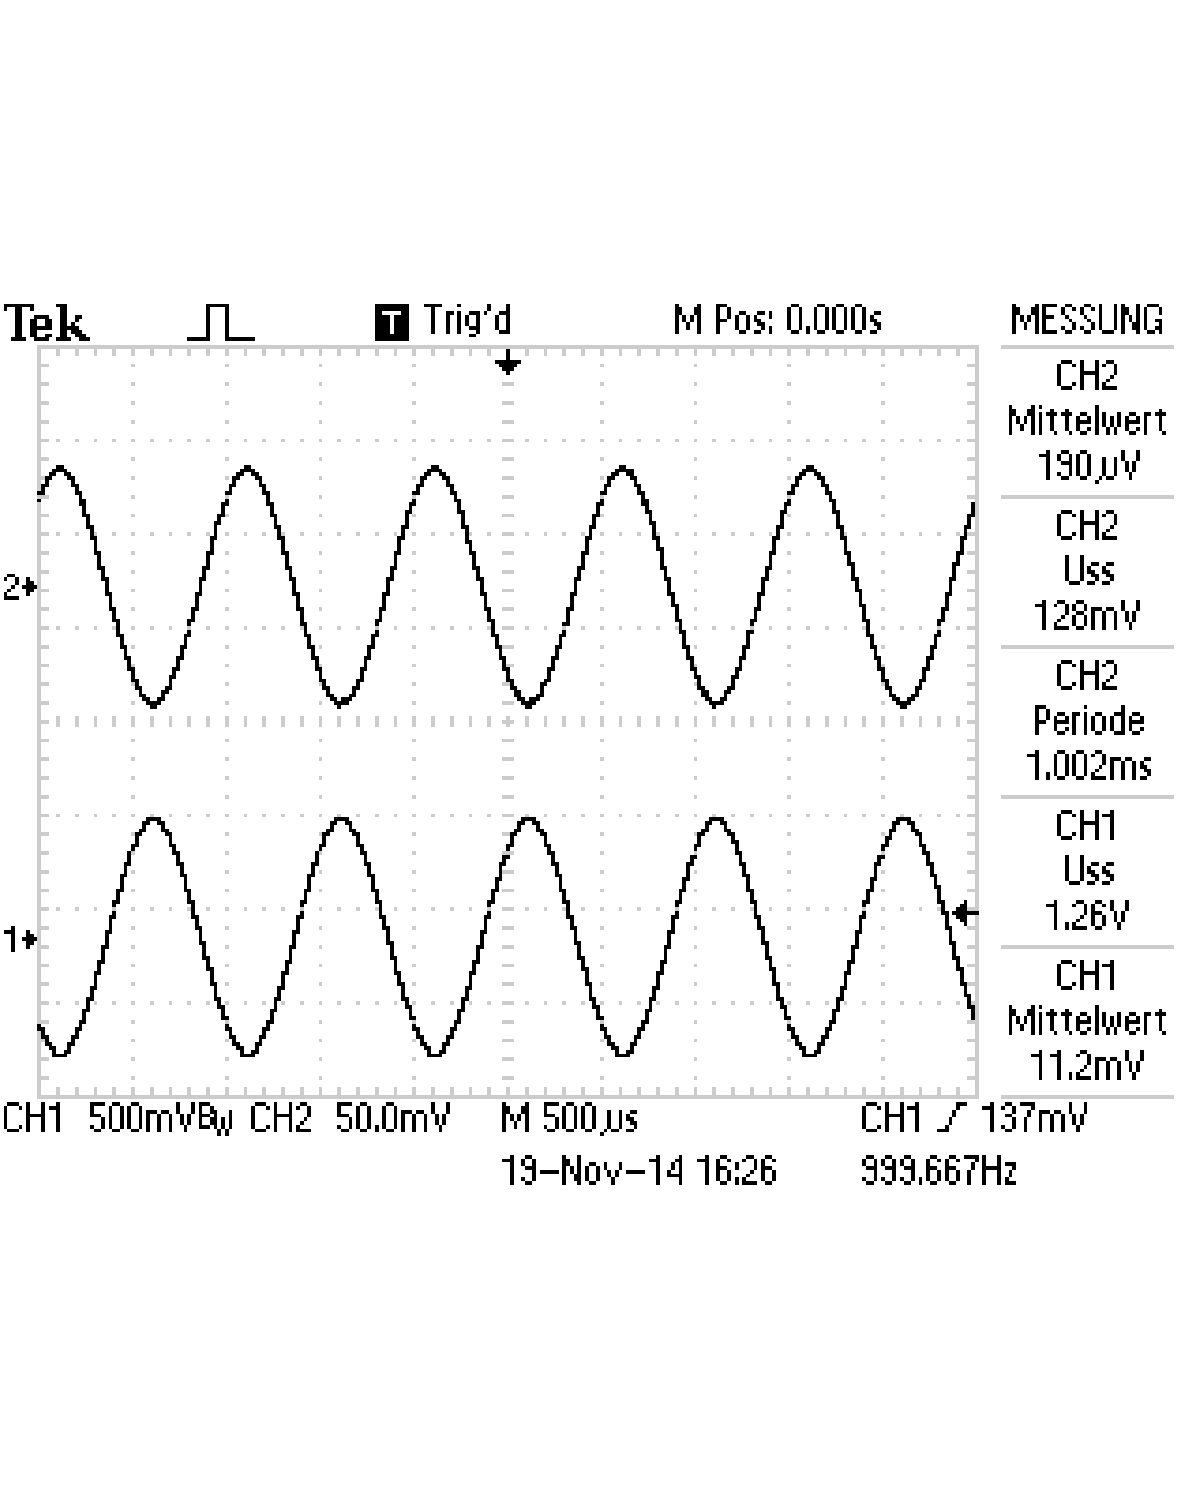
\includegraphics[width=\textwidth , scale = 0.4]{2_4_10_1k.pdf}
                \caption[Aufnahme des Signals bei 1kHz]{Aufnahme des Signals bei 1kHz}
                \label{fig:2_4_10_1k}
        \end{subfigure}%
       % ~ %add desired spacing between images, e. g. ~, \quad, \qquad, \hfill etc.
          %(or a blank line to force the subfigure onto a new line)
        \hfill
        \begin{subfigure}[b]{0.28\textwidth}
                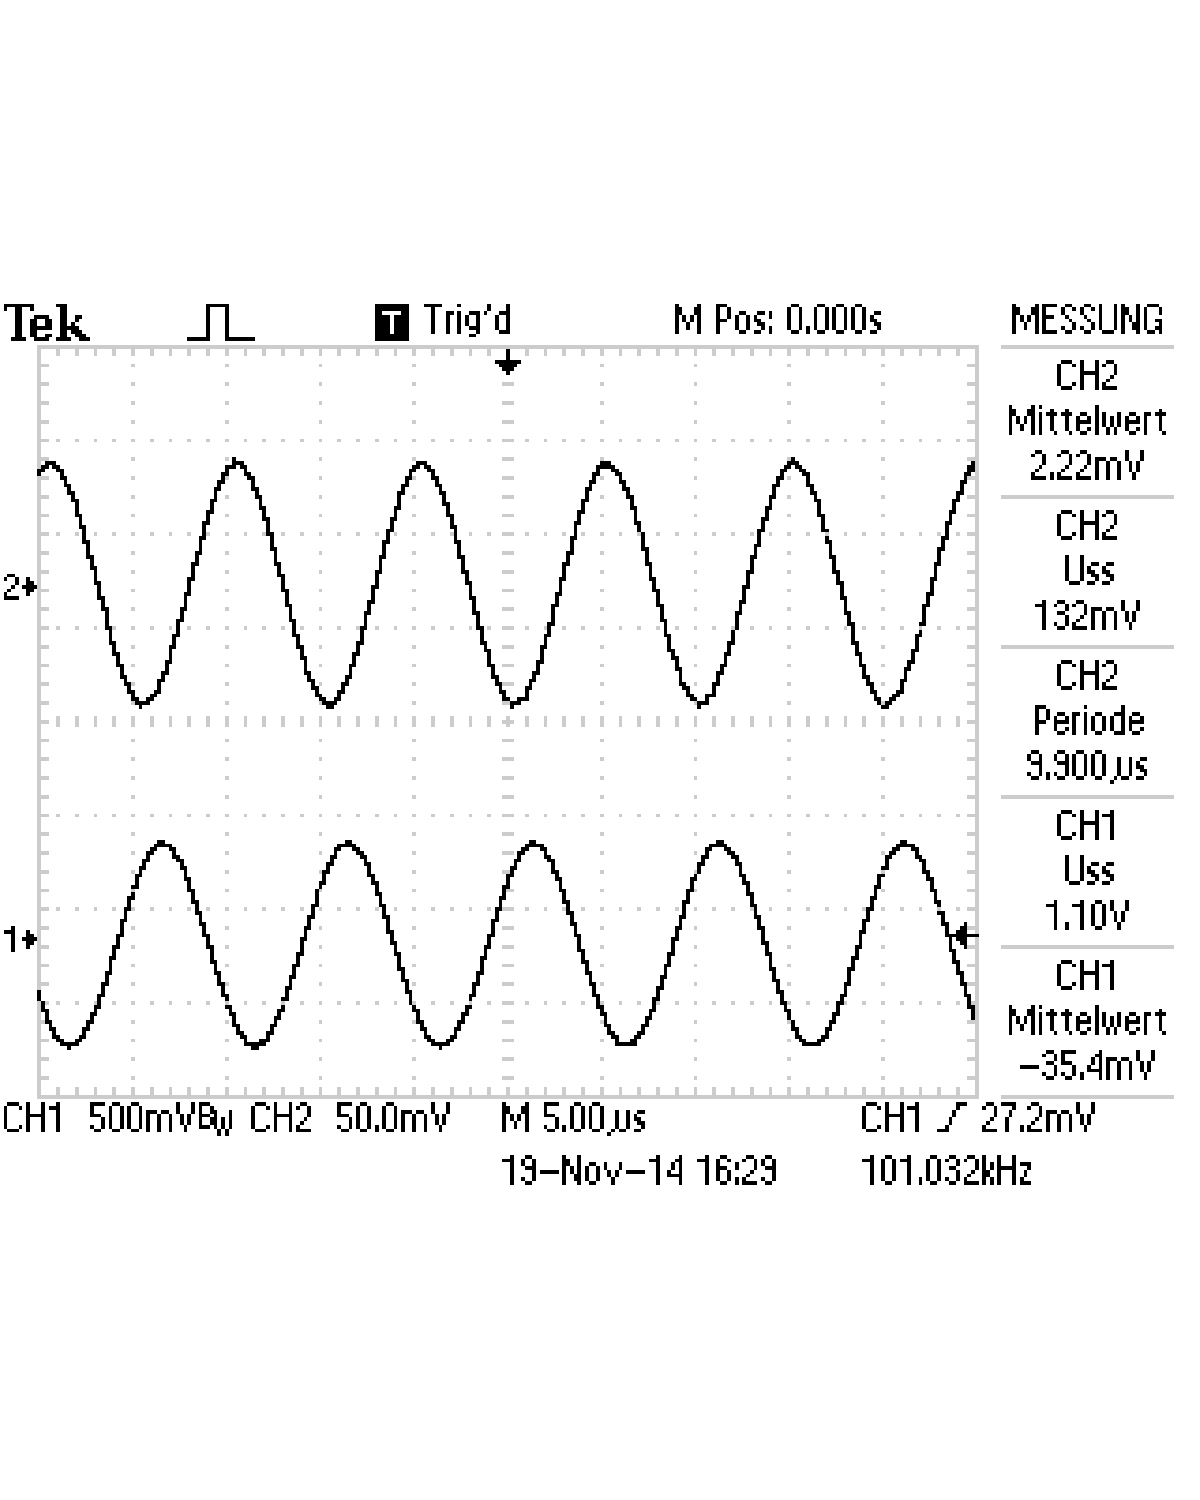
\includegraphics[width=\textwidth , scale = 0.4]{2_4_10_100k.pdf}
                \caption[Aufnahme des Signals bei 100kHz]{Aufnahme des Signals bei 100kHz}
                \label{fig:2_4_10_100k}
        \end{subfigure}
       % ~ %add desired spacing between images, e. g. ~, \quad, \qquad, \hfill etc.
          %(or a blank line to force the subfigure onto a new line)
        \hfill
        \begin{subfigure}[b]{0.28\textwidth}
                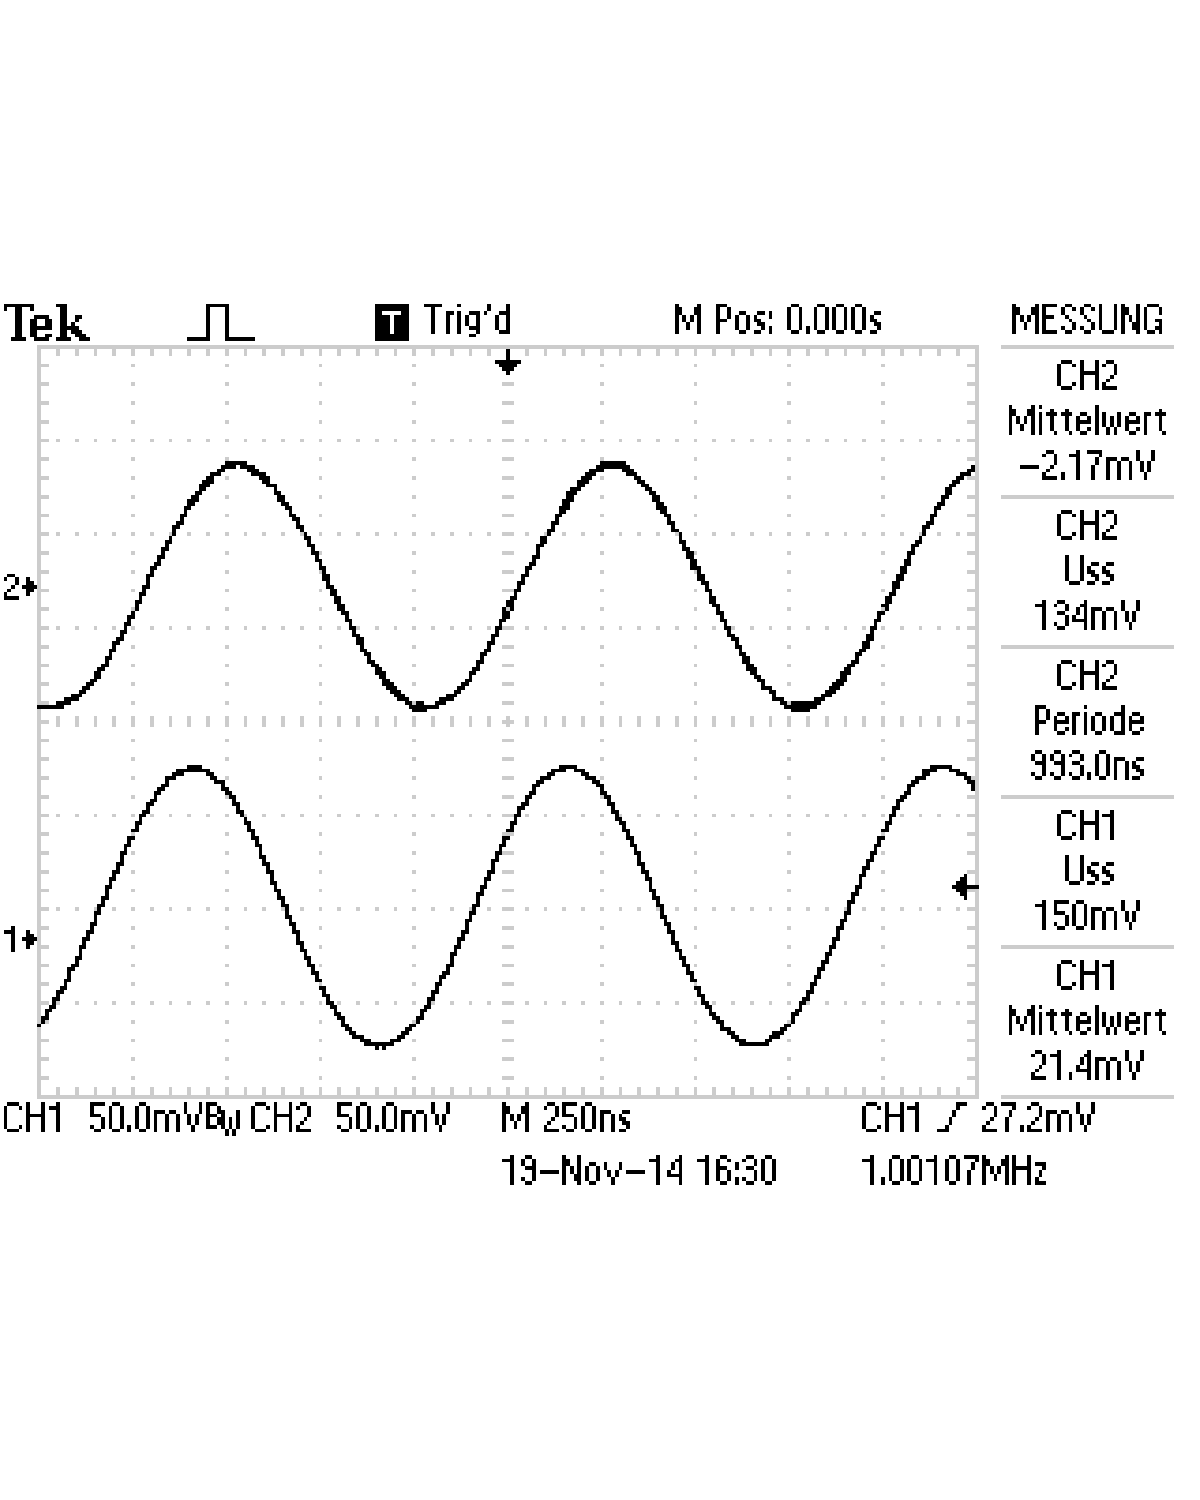
\includegraphics[width=\textwidth , scale = 0.4]{2_4_10_1m.pdf}
                \caption[Aufnahme des Signals bei 1mHz]{Aufnahme des Signals bei 1mHz}
  				\label{fig:2_4_10_1m}
        \end{subfigure}
        \caption{Kurven für 1kHz, 100kHz und 1mHz, bei einer Verstärkung von -10}
        \label{fig:2_4_10}
\end{figure}


\begin{figure}[H]
        \centering
        \begin{subfigure}[b]{0.28\textwidth}
                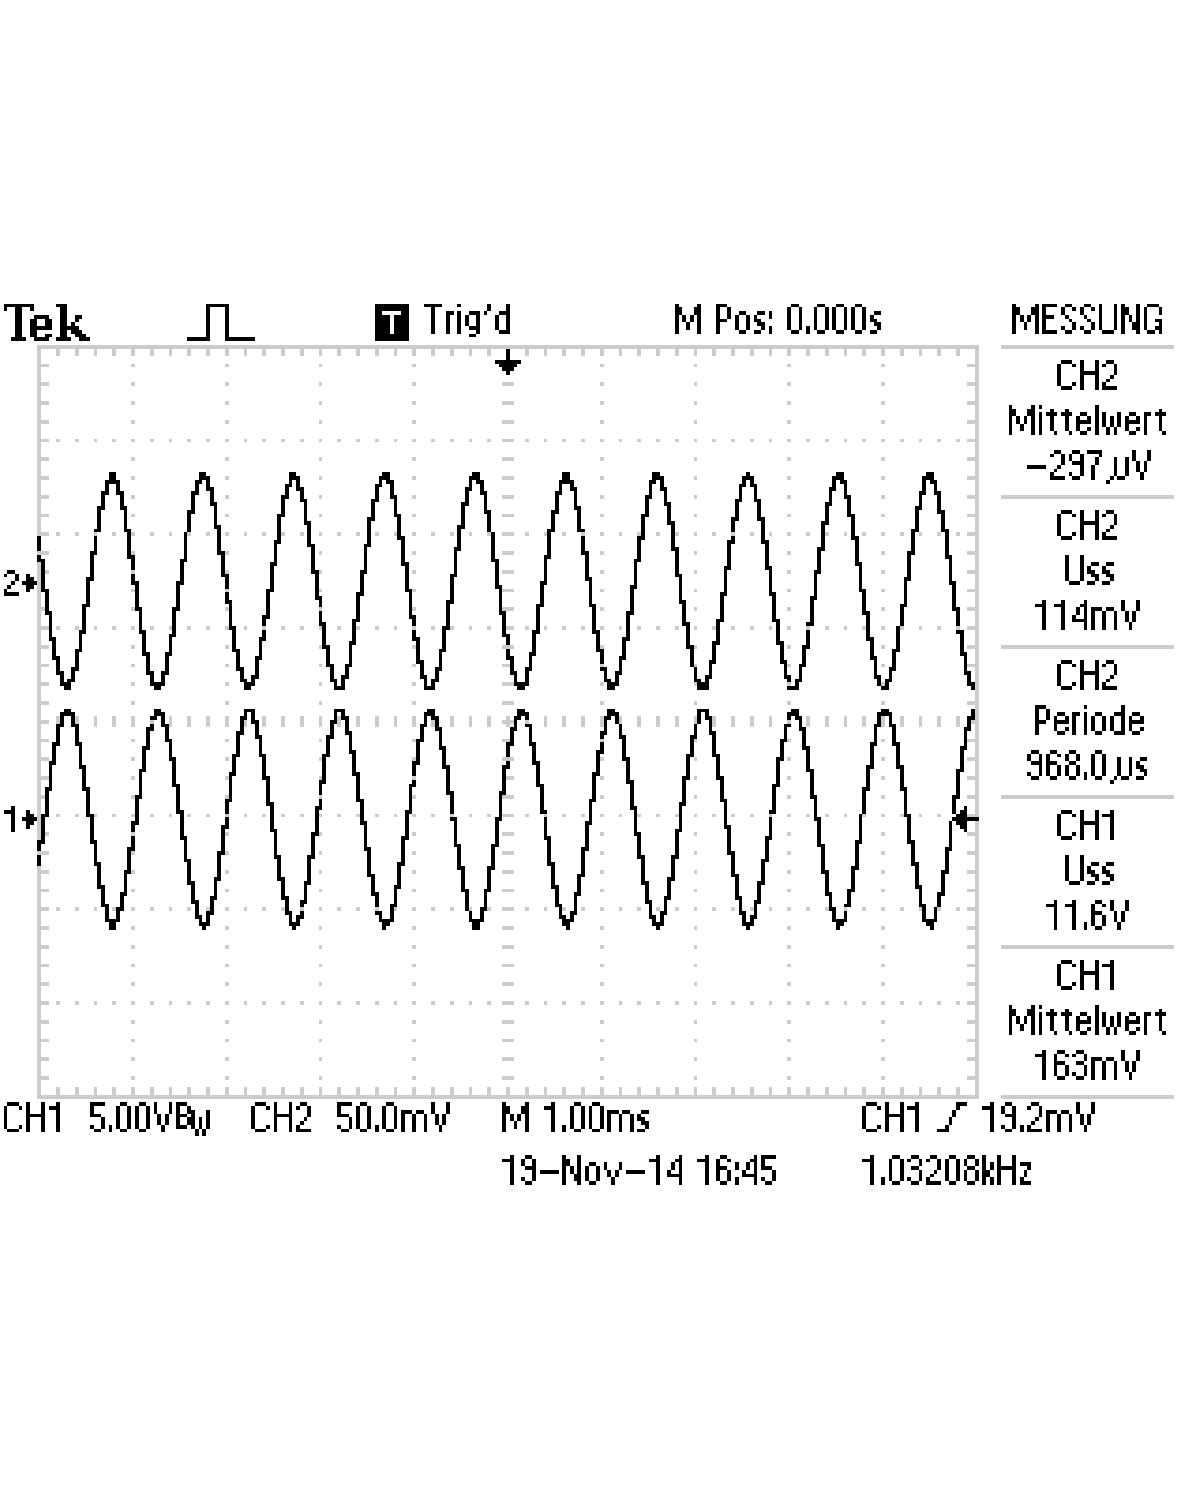
\includegraphics[width=\textwidth , scale = 0.4]{2_4_100_1k.pdf}
                \caption[Aufnahme des Signals bei 1kHz]{Aufnahme des Signals bei 1kHz}
                \label{fig:2_4_100_1k}
        \end{subfigure}%
       % ~ %add desired spacing between images, e. g. ~, \quad, \qquad, \hfill etc.
          %(or a blank line to force the subfigure onto a new line)
        \hfill
        \begin{subfigure}[b]{0.28\textwidth}
                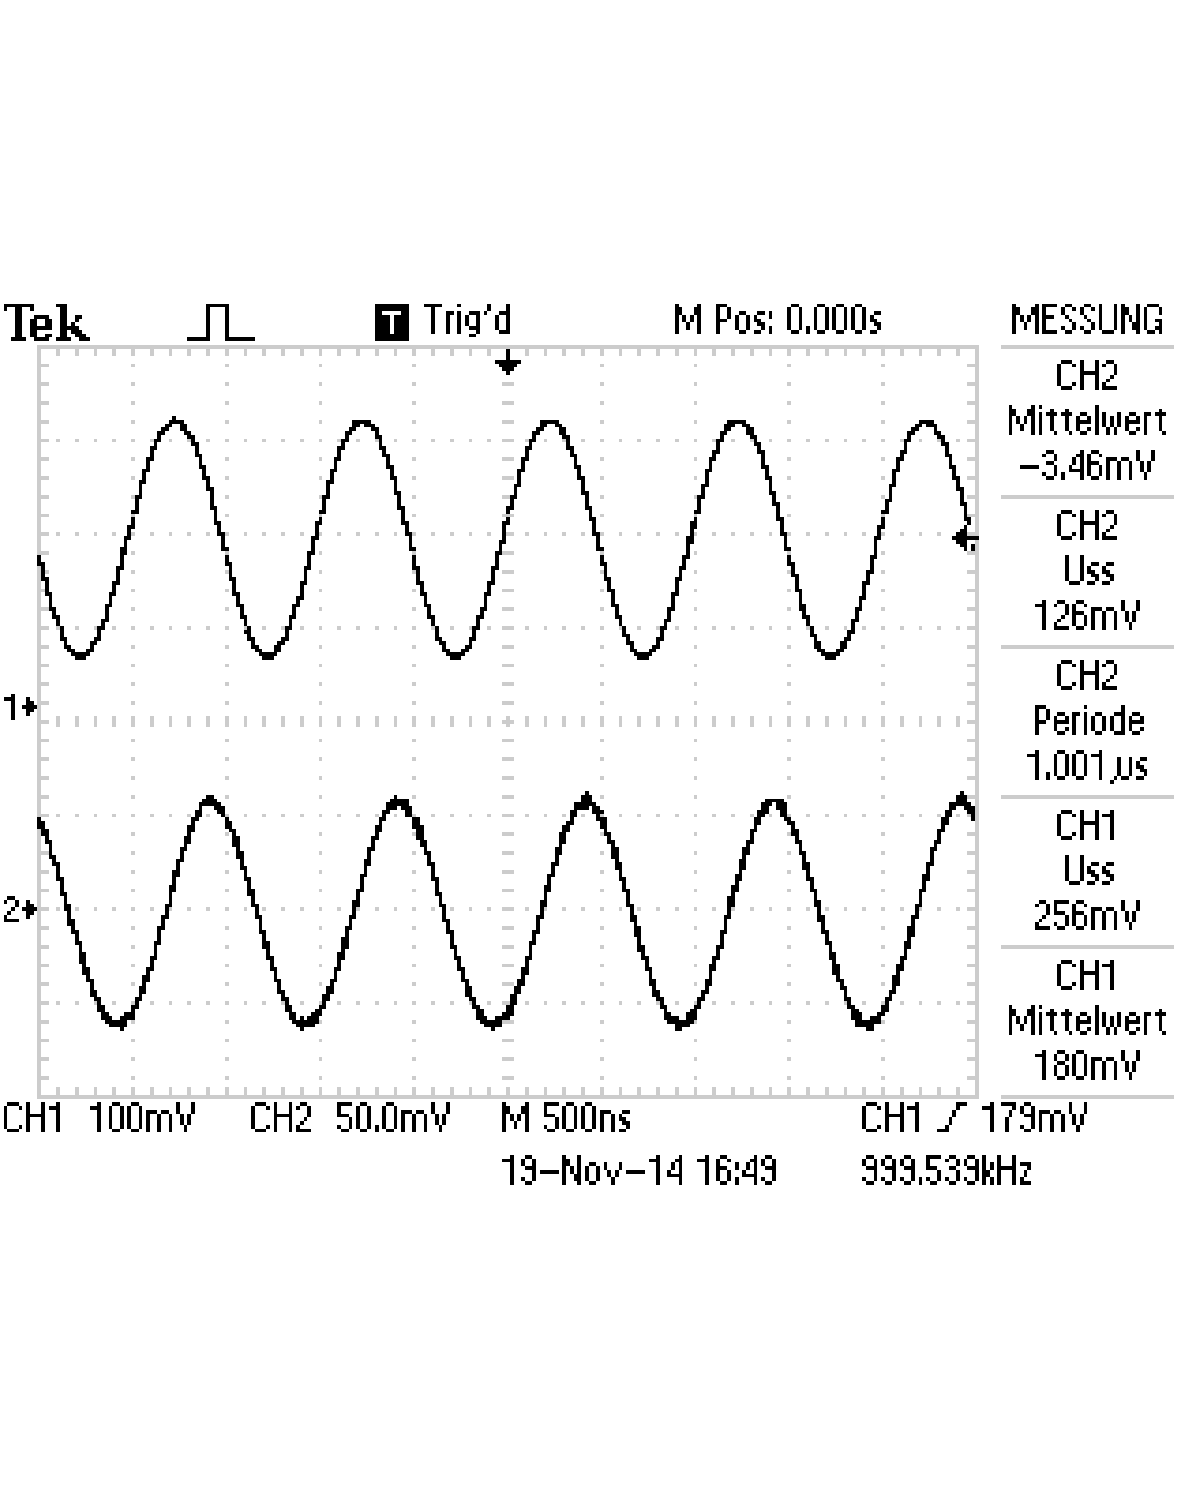
\includegraphics[width=\textwidth , scale = 0.4]{2_4_100_100k.pdf}
                \caption[Aufnahme des Signals bei 100kHz]{Aufnahme des Signals bei 100kHz}
                \label{fig:2_4_100_100k}
        \end{subfigure}
       % ~ %add desired spacing between images, e. g. ~, \quad, \qquad, \hfill etc.
          %(or a blank line to force the subfigure onto a new line)
        \hfill
        \begin{subfigure}[b]{0.28\textwidth}
                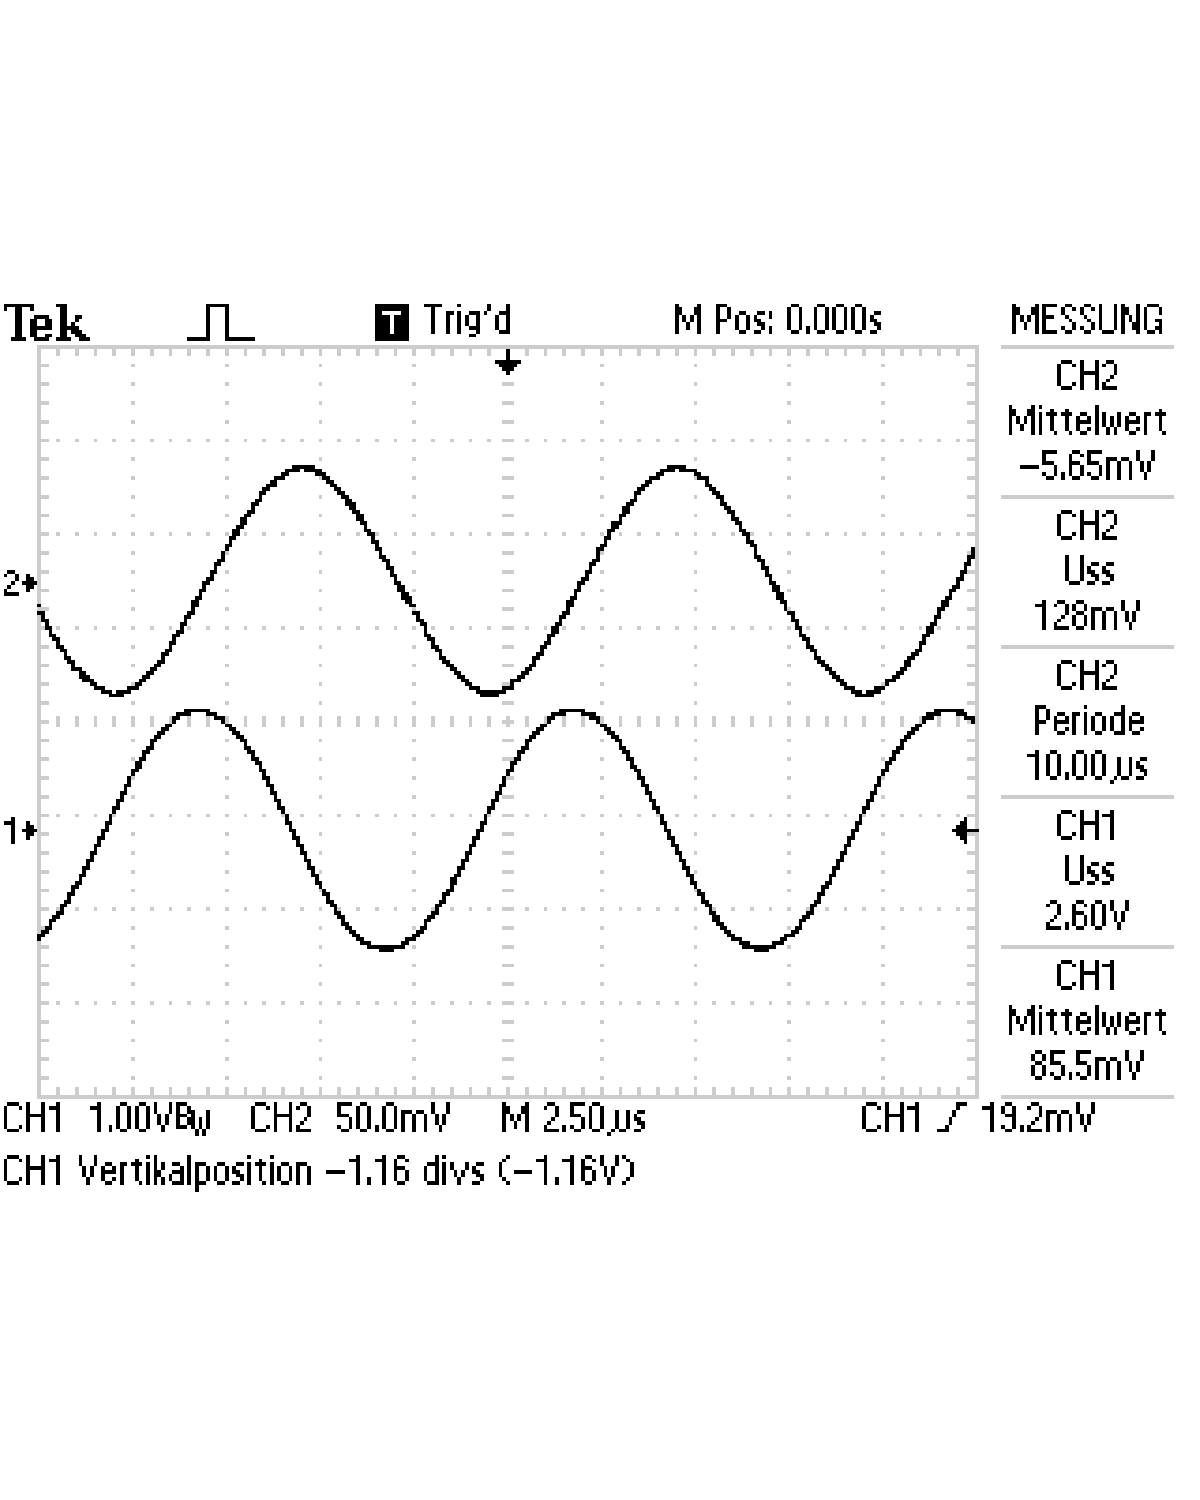
\includegraphics[width=\textwidth , scale = 0.4]{2_4_100_1m.pdf}
                \caption[Aufnahme des Signals bei 1mHz]{Aufnahme des Signals bei 1mHz}
  				\label{fig:2_4_100_1m}
        \end{subfigure}
        \caption{Kurven für 1kHz, 100kHz und 1mHz, bei einer Verstärkung von -100}
        \label{fig:2_4_100}
\end{figure}



\subsection{Diskussion}
%(immer) die gemessenen werte und die bestimmten werte über die messfehler mit literaturwerten oder untereinander vergleichen
%in welchem fehlerintervall des messwertes liegt der literaturwert oder der vergleichswert?
%wie ist der relative anteil des fehlers am messwert und damit die qualität unserer messung?
%in einem satz erklären, wie gut unser fehler und damit unsere messung ist
%kurz erläutern, wie systematische fehler unsere messung beeinflusst haben könnten
%(wichtig) zum schluss ansprechen, in wie weit die ergebnisse mit der theoretischen vorhersage übereinstimmen
%--------------------------------------------------------------------------------------------
%falls tabellen mit den messwerten zu lang werden, kann die section mit den messwerten auch hinter der diskussion angefügt bzw. eine section mit dem anhang eingefügt werden.
%1-----------------------------------------------1

Wie erwartet lies sich das eingehende Spannungssignal bei kleinen Frequenzen invertierten, bei hohen Frequenzen trat jedoch noch eine zusätzliche Verschiebung des Signals auf.

\section{Differenzierer}
%kurz das ziel dieses versuchsteiles ansprechen, damit keine zwei überschriften direkt übereinander stehen!
%bei schwierigeren versuchen kann auch der theoretische hintergrund erläutert werden. (mit formeln, herleitungen und erklärungen)
Mit der Schaltung in diesem Versuchsteil kann das Eingangssignal differenziert werden.
\subsection{Verwendete Geräte}
%(immer) eine skizze oder ein foto einfügen, die geräte/materialien !nummerieren! und z.b. eine legende dazu schreiben, besser wäre es das ganze in einem Fließtext gut zu beschreiben.
%falls am anfang des versuches nicht klar ist, was alles verwendet wird, wenn möglich erst am ende ein großes foto von den verwendeten materialien machen!\\

Verwendet werden ein Operationsverstärker, ein Funktionsgenerator, ein Kondensator,ein Widerstand und DVMs.

\subsection{Verwendete Formeln}
%eine legende kann angefertigt werden, die selbstverständlichen buchstaben müssen nicht extra erklärt werden
%mit knappen erklärungen die !verwendeten! formeln, sowie die zugehörige fehlerrechnung einfügen
%2-----------------------------------------------2
Mit der Formel
\begin{align}
U_a = -CR_f\frac{dU_f}{dt}
\end{align}
welche sich aus der Knotenregel und der Definition der Kapazität ergibt, kann die Ausgangsspannung berechnet werden.
%ab hier kann nochmal in einzelne versuchsteile unterteilt werden
\subsection{Versuchsaufbau}
%skizze zum versuchsaufbau (oder foto) einfügen,   es muss erklärt werden wie das ganze funktioniert und welche speziellen einstellungen verwendet wurden (z.b. welche knöpfe an den geräten für die messung verdreht wurden)

C ist ein 0,1$\mu$F, R ein 10k$\Omega$ Widerstand, der Funktionsgenerator FG wird mit 100Hz betrieben.

\begin{figure}[H] 
  \centering
    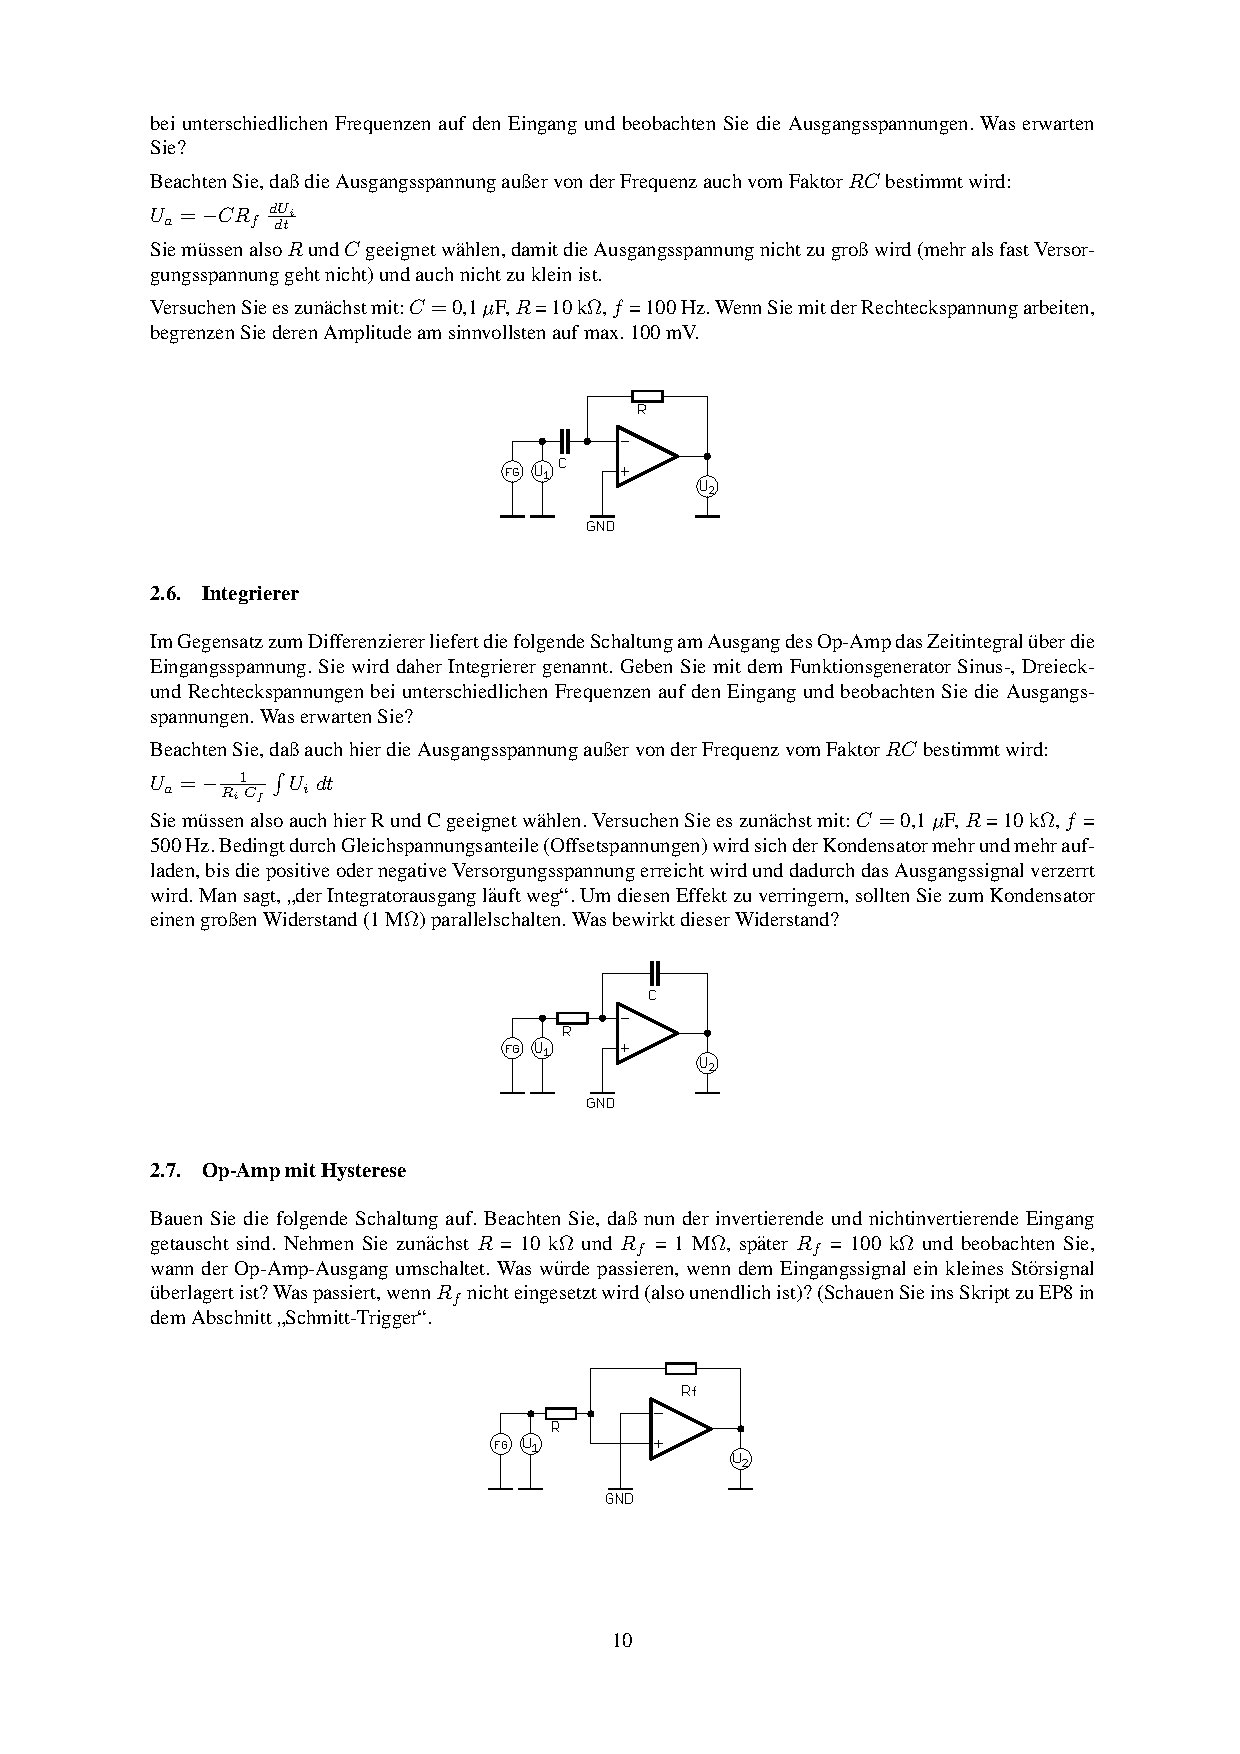
\includegraphics[trim = 10mm 200mm 10mm 60mm, clip, scale = 1]{ep4_14[Page10].pdf}
  	\caption[Schaltskizze des Differenzierers]{Schaltskizze des Differenzierers\footnotemark}
  \label{fig:1}
\end{figure}
\footnotetext{Abbildung entnommen von http://www.atlas.uni-wuppertal.de/$\sim$kind/ep4\_14.pdf Seite 10 am 17.11.2014}

\subsection{Versuchsdurchführung}
%erklären, !was! wir machen, !warum! wir das machen und mit welchem ziel
%(wichtig) präzize erklären, wie bei dem versuch vorgegangen und was gemacht wurde
Diese Schaltung liefert als Ausgangssignal die zeitliche Änderung der Eingangsspannung und wird daher 'Differenzierer' genannt. Die Herleitung dieser Beziehung folgt aus der Knotenregel und der Definition der Kapazität. Bei Sinus-, Dreieck- und Rechteckspannung und bei unterschiedlichen Frequenzen soll die Ausgangsspannung beobachtet und mit dem Oszilloskop aufgezeichnet werden.(angefangen bei $f$ = \unit[100]{Hz})

\subsection{Auswertung}
%zuerst !alle! errechneten werte entweder in ganzen sätzen aufzählen, oder in tabellen (übersichtlicher) dargestellen, sowie auf die verwendeten formeln verweisen (die referenzierung der formel kann in der überschrift stehen)
%kurz erwähnen (vor der tabelle), warum wir das ganze ausrechnen bzw. was wir dort ausrechnen
%danach histogramme und plots erstellen, wobei wenn möglich funktionen durch die plots gelegt werden (zur not können auch splines benutzt werden, was aber angegeben werden muss)
%bei fits immer die funktion und das reduzierte chiquadrat mit angegeben, wobei auf verständlichkeit beim entziffern der zehnerpotenzen geachtet werden muss z.b. f(x)=(wert+-fehler)\cdot10^{irgendeine zahl}\cdot x + (wert+-fehler)\cdot10^{irgendeine zahl}
%bei jedem fit erklären, nach welchem zusammenhang gefittet wurde und warum!
%bei plots darauf achten, dass die achsenbeschriftung (auch die tics) die richtige größe haben und die legende im plot nicht die messwerte verdeckt
%kurz die aufgabenstellung abhandeln
%2-----------------------------------------------2

Im Versuchsteil 2.5 sollte die Eigenschafte des Op-Amp als Differenzierer untersucht werden. Die aufgenommenen Kurven sind in Abbildung \ref{fig:2_5_drei}, Abbildung \ref{fig:2_5_recht} und Abbildung \ref{fig:2_5_sin} zu sehen. Es ist zu erkennen, das für hohe Frequenzen das Eingangssignal nicht mehr richtig Differenziert wird. Bei kleinen Frequenzen klappt dies aber noch sehr gut. Beispielhaft wurde die erwartet Ausgangsspannung für das Rechtecksignal bei 100 Hz bestimmt. Der Faktor C$\cdot$RF ist gleich 1, auf 5 ms (ein Kästchen in x-Richtung) kommt ein Anstieg von 270 mV, daraus ergebt sich eine Steigung von 54 V die entspricht in etwa der halben Höhe des Ausgangssignals. Es darf nicht der Uss Wert des Oszilloskops für die Ausgangsspannung genommen werden, da die Überschwinger mit gemessen werden.


\begin{figure}[H]
        \centering
        \begin{subfigure}[b]{0.28\textwidth}
                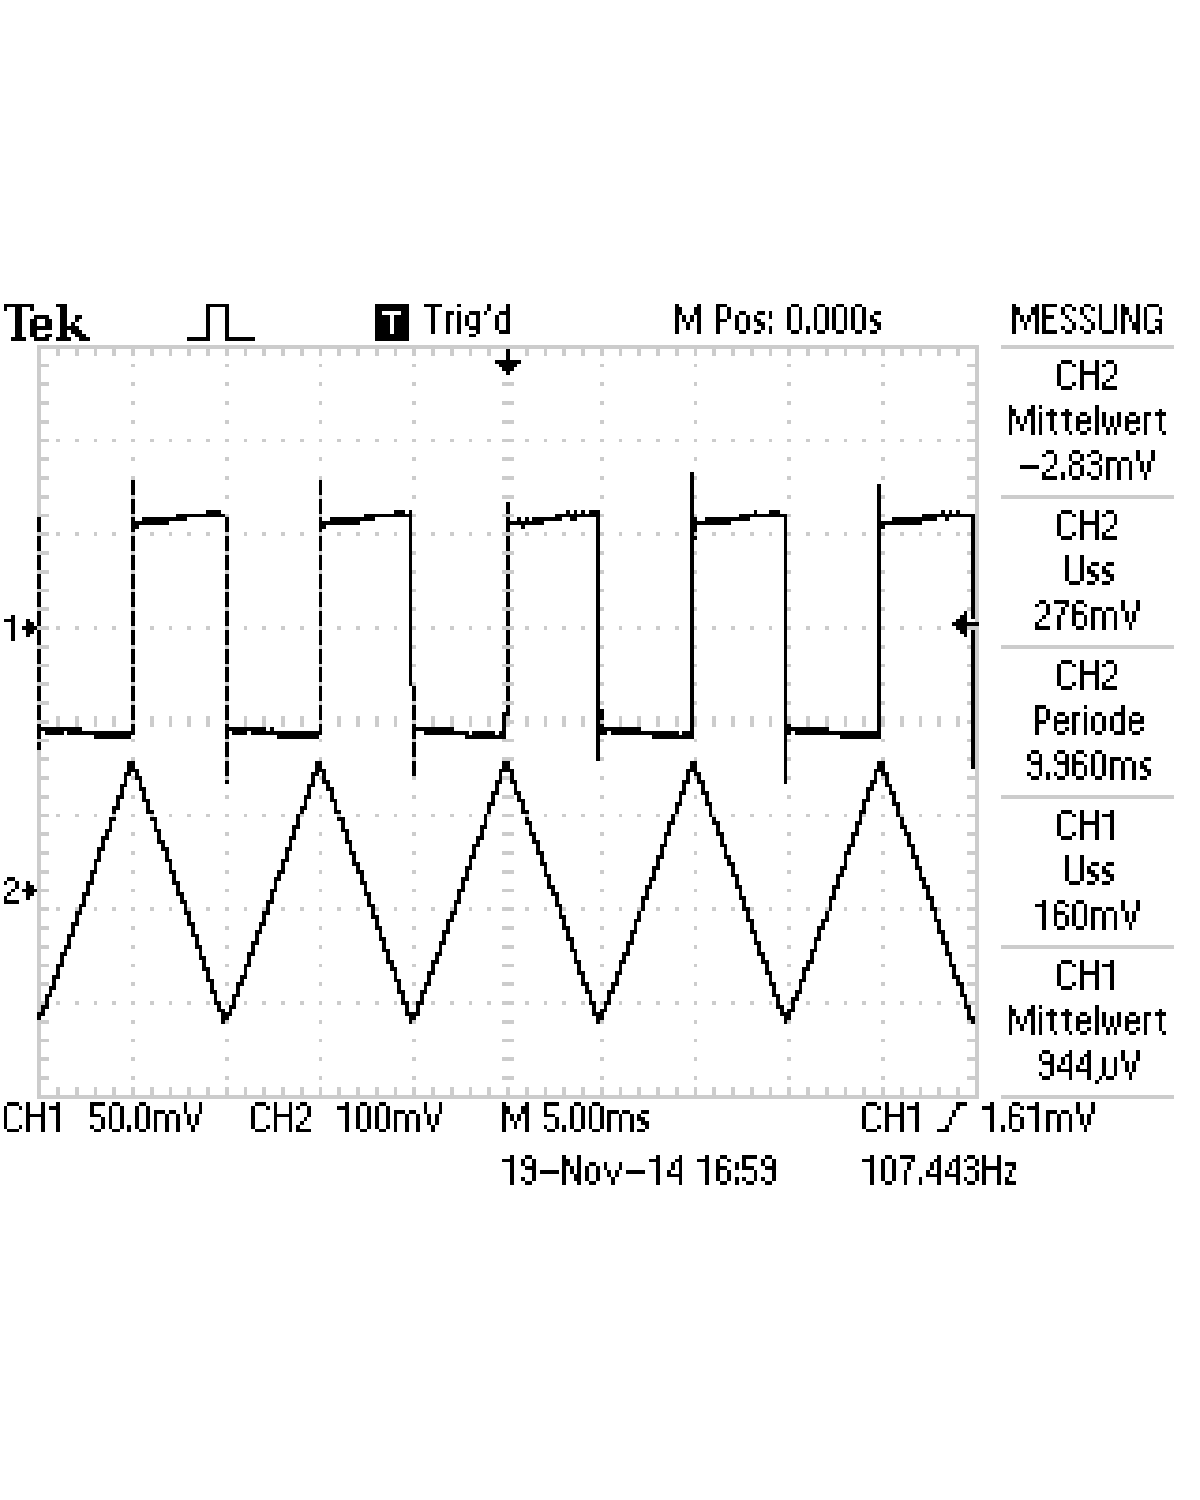
\includegraphics[width=\textwidth , scale = 0.4]{2_5_drei_100.pdf}
                \caption[Aufnahme des Signals bei 100Hz]{Aufnahme des Signals bei 100Hz}
                \label{fig:2_5_drei_100}
        \end{subfigure}%
       % ~ %add desired spacing between images, e. g. ~, \quad, \qquad, \hfill etc.
          %(or a blank line to force the subfigure onto a new line)
        \hfill
        \begin{subfigure}[b]{0.28\textwidth}
                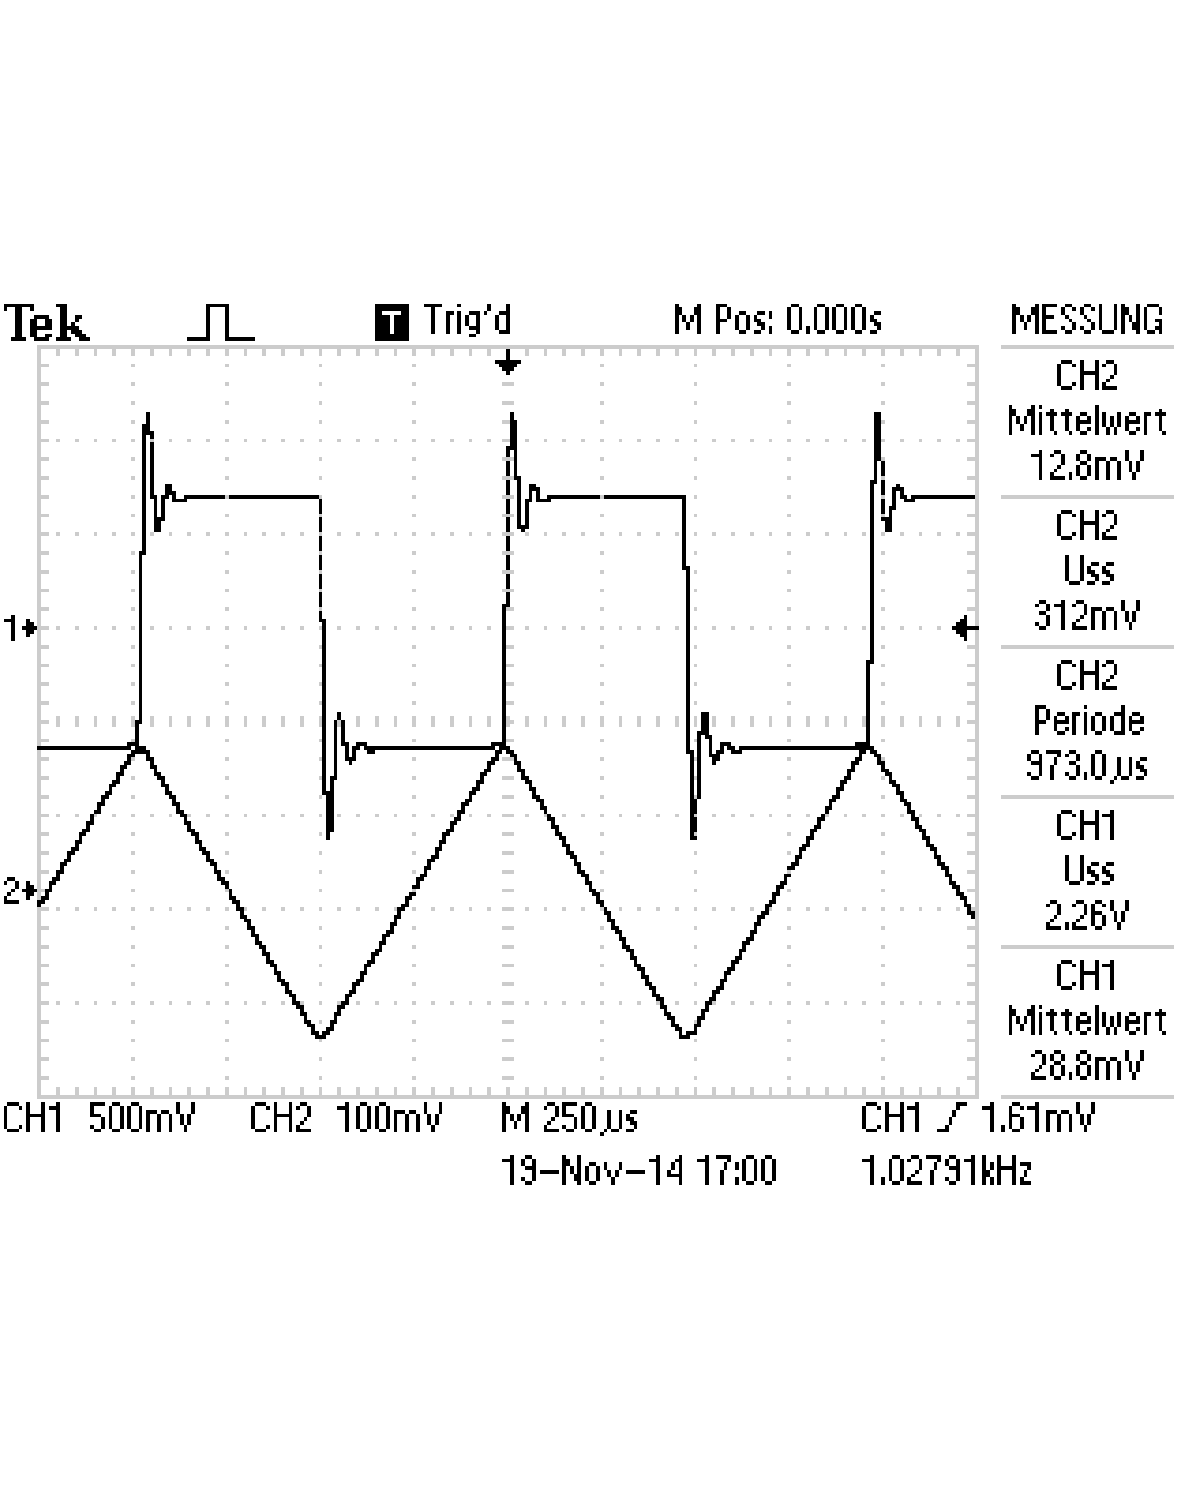
\includegraphics[width=\textwidth , scale = 0.4]{2_5_drei_1k.pdf}
                \caption[Aufnahme des Signals bei 1kHz]{Aufnahme des Signals bei 1kHz}
                \label{fig:2_5_drei_1k}
        \end{subfigure}
       % ~ %add desired spacing between images, e. g. ~, \quad, \qquad, \hfill etc.
          %(or a blank line to force the subfigure onto a new line)
        \hfill
        \begin{subfigure}[b]{0.28\textwidth}
                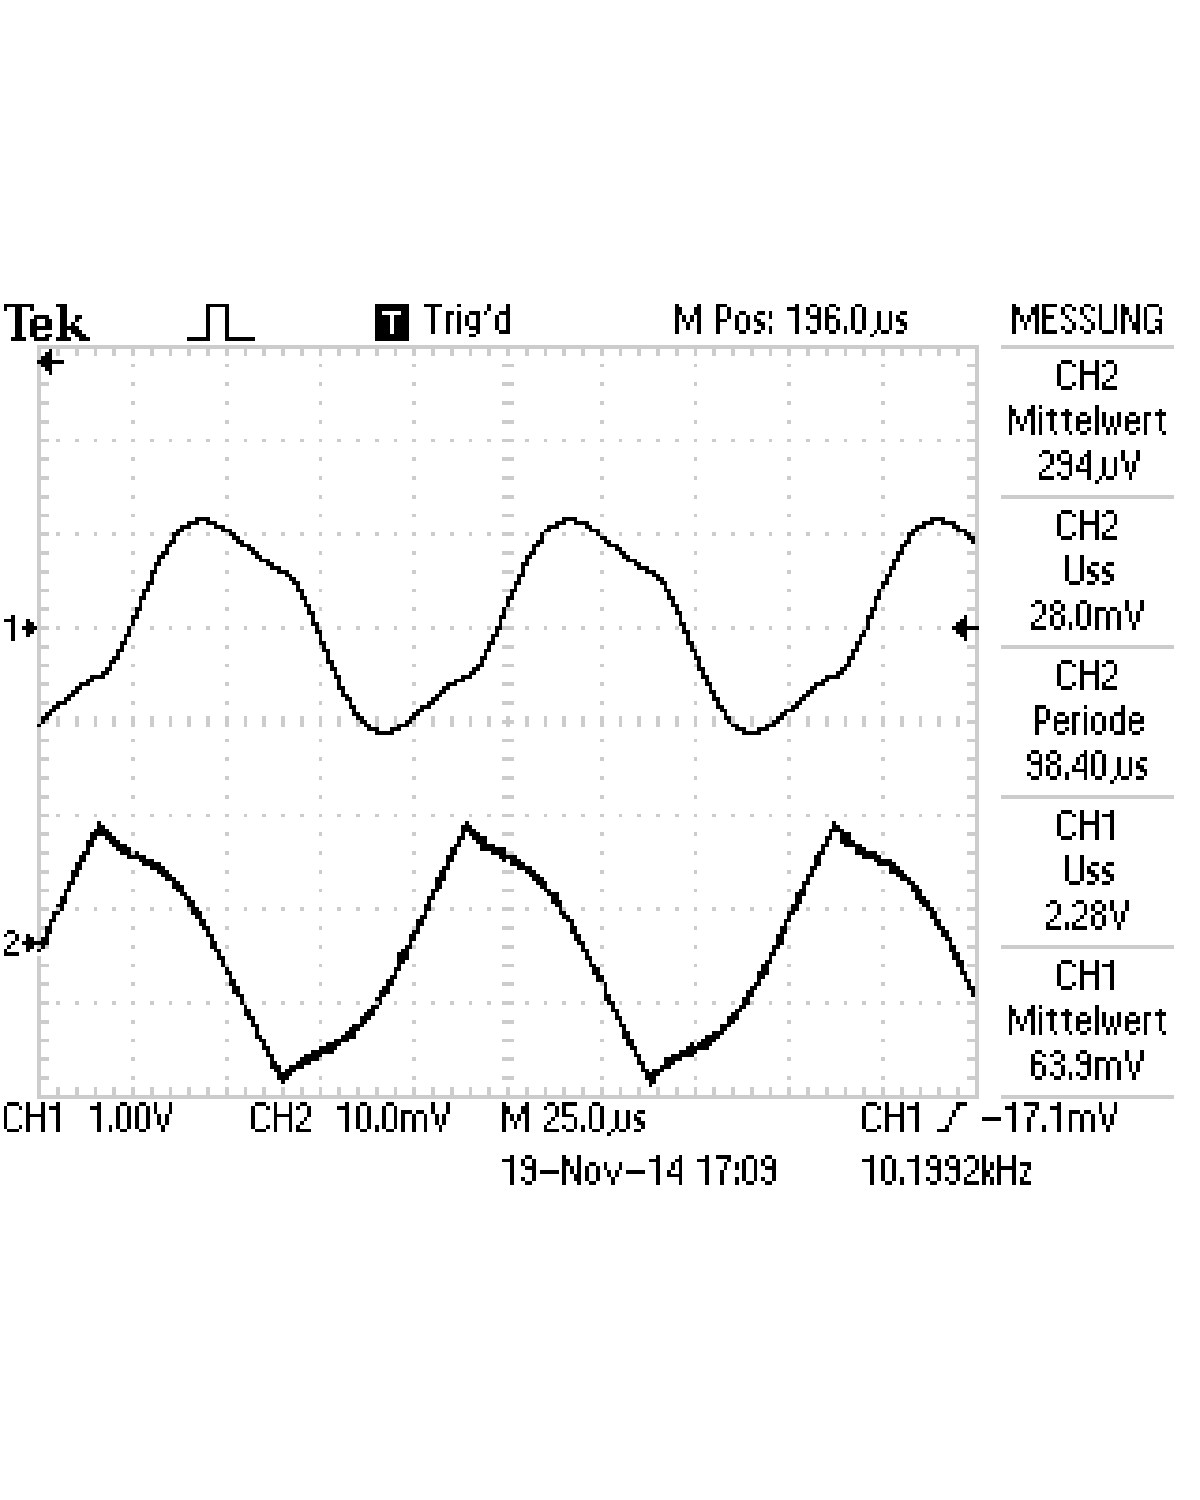
\includegraphics[width=\textwidth , scale = 0.4]{2_5_drei_10k.pdf}
                \caption[Aufnahme des Signals bei 10kHz]{Aufnahme des Signals bei 10kHz}
  				\label{fig:2_5_drei_10k}
        \end{subfigure}
        \caption{Kurven für 100Hz, 1kHz und 10kHz, bei einer Dreiecksspannung}
        \label{fig:2_5_drei}
\end{figure}




\begin{figure}[H]
        \centering
        \begin{subfigure}[b]{0.28\textwidth}
                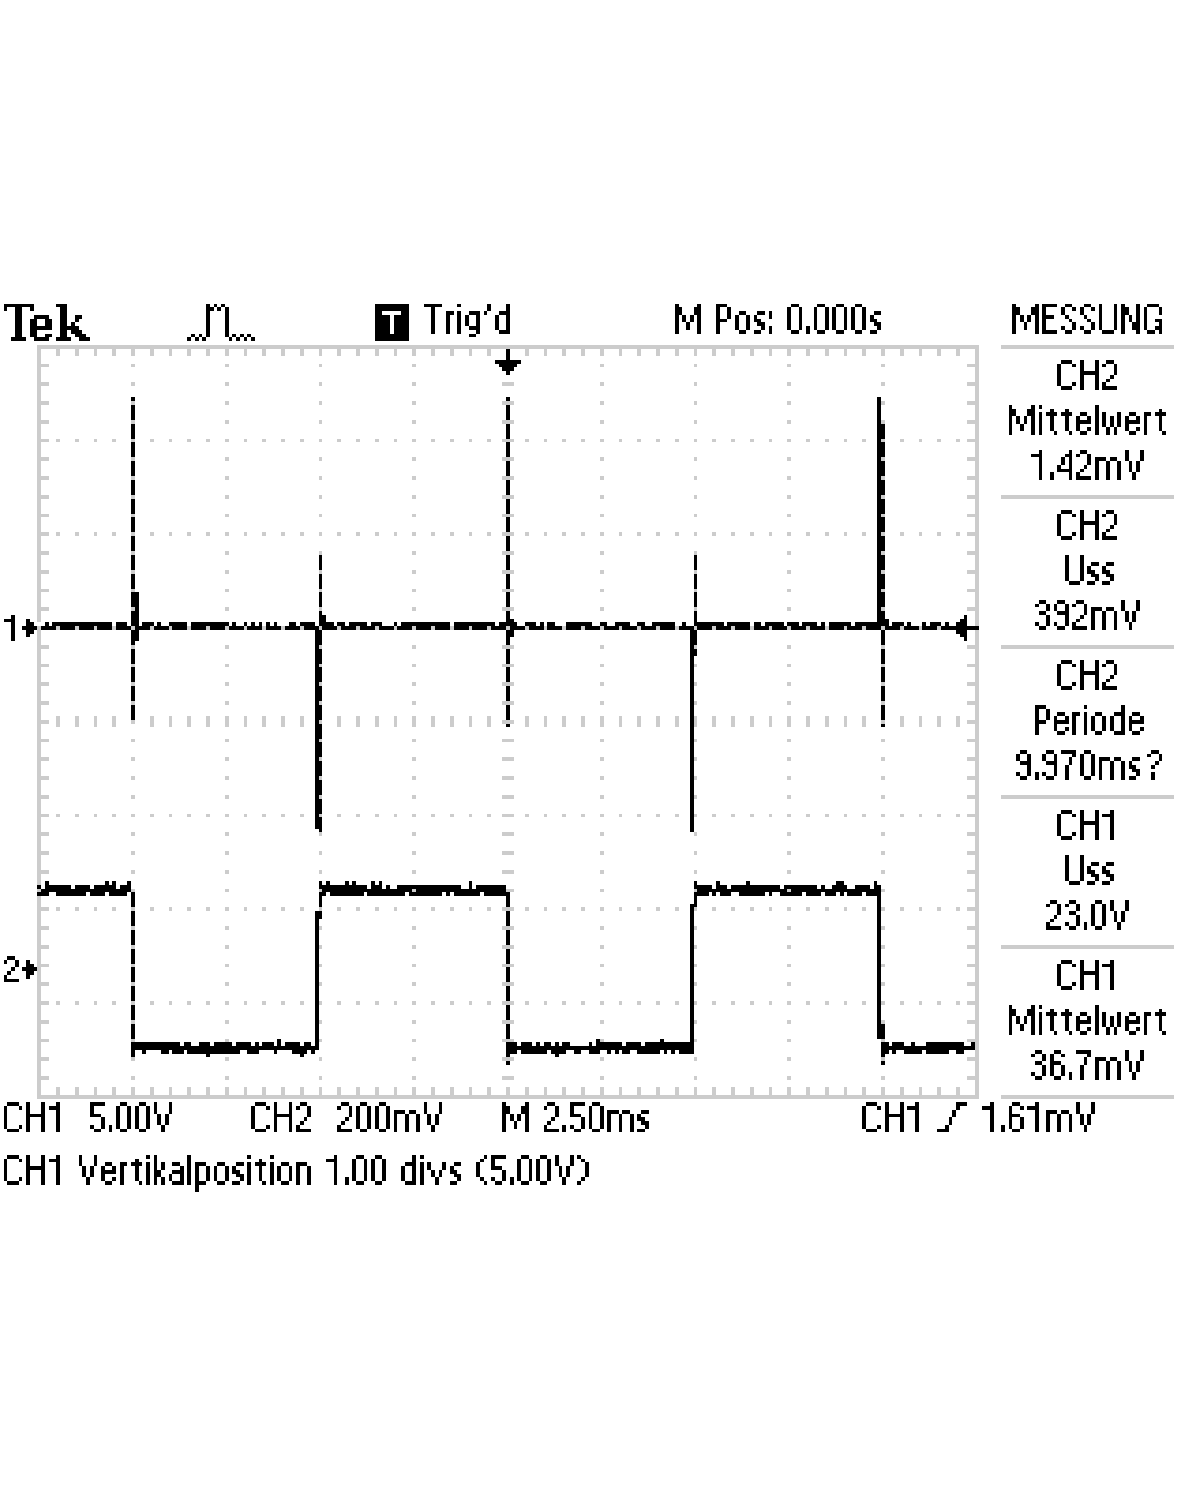
\includegraphics[width=\textwidth , scale = 0.4]{2_5_recht_100.pdf}
                \caption[Aufnahme des Signals bei 100Hz]{Aufnahme des Signals bei 100Hz}
                \label{fig:2_5_recht_100}
        \end{subfigure}%
       % ~ %add desired spacing between images, e. g. ~, \quad, \qquad, \hfill etc.
          %(or a blank line to force the subfigure onto a new line)
        \hfill
        \begin{subfigure}[b]{0.28\textwidth}
                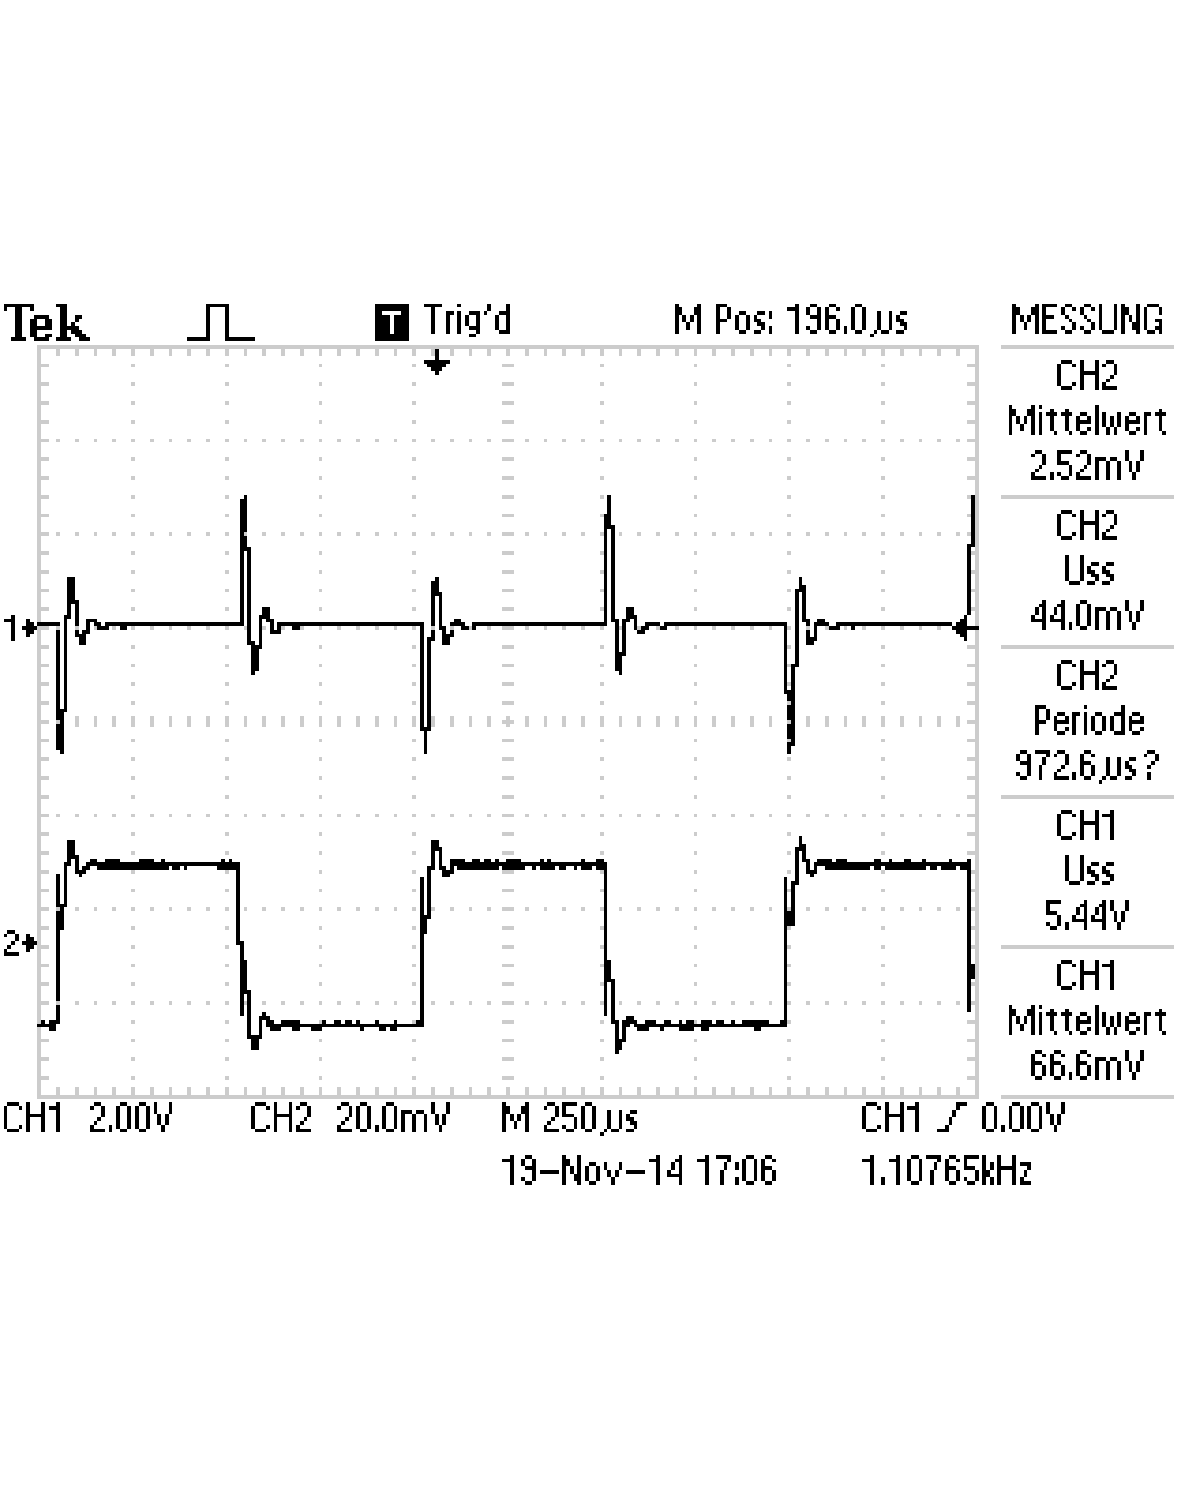
\includegraphics[width=\textwidth , scale = 0.4]{2_5_recht_1k.pdf}
                \caption[Aufnahme des Signals bei 1kHz]{Aufnahme des Signals bei 1kHz}
                \label{fig:2_5_recht_1k}
        \end{subfigure}
       % ~ %add desired spacing between images, e. g. ~, \quad, \qquad, \hfill etc.
          %(or a blank line to force the subfigure onto a new line)
        \hfill
        \begin{subfigure}[b]{0.28\textwidth}
                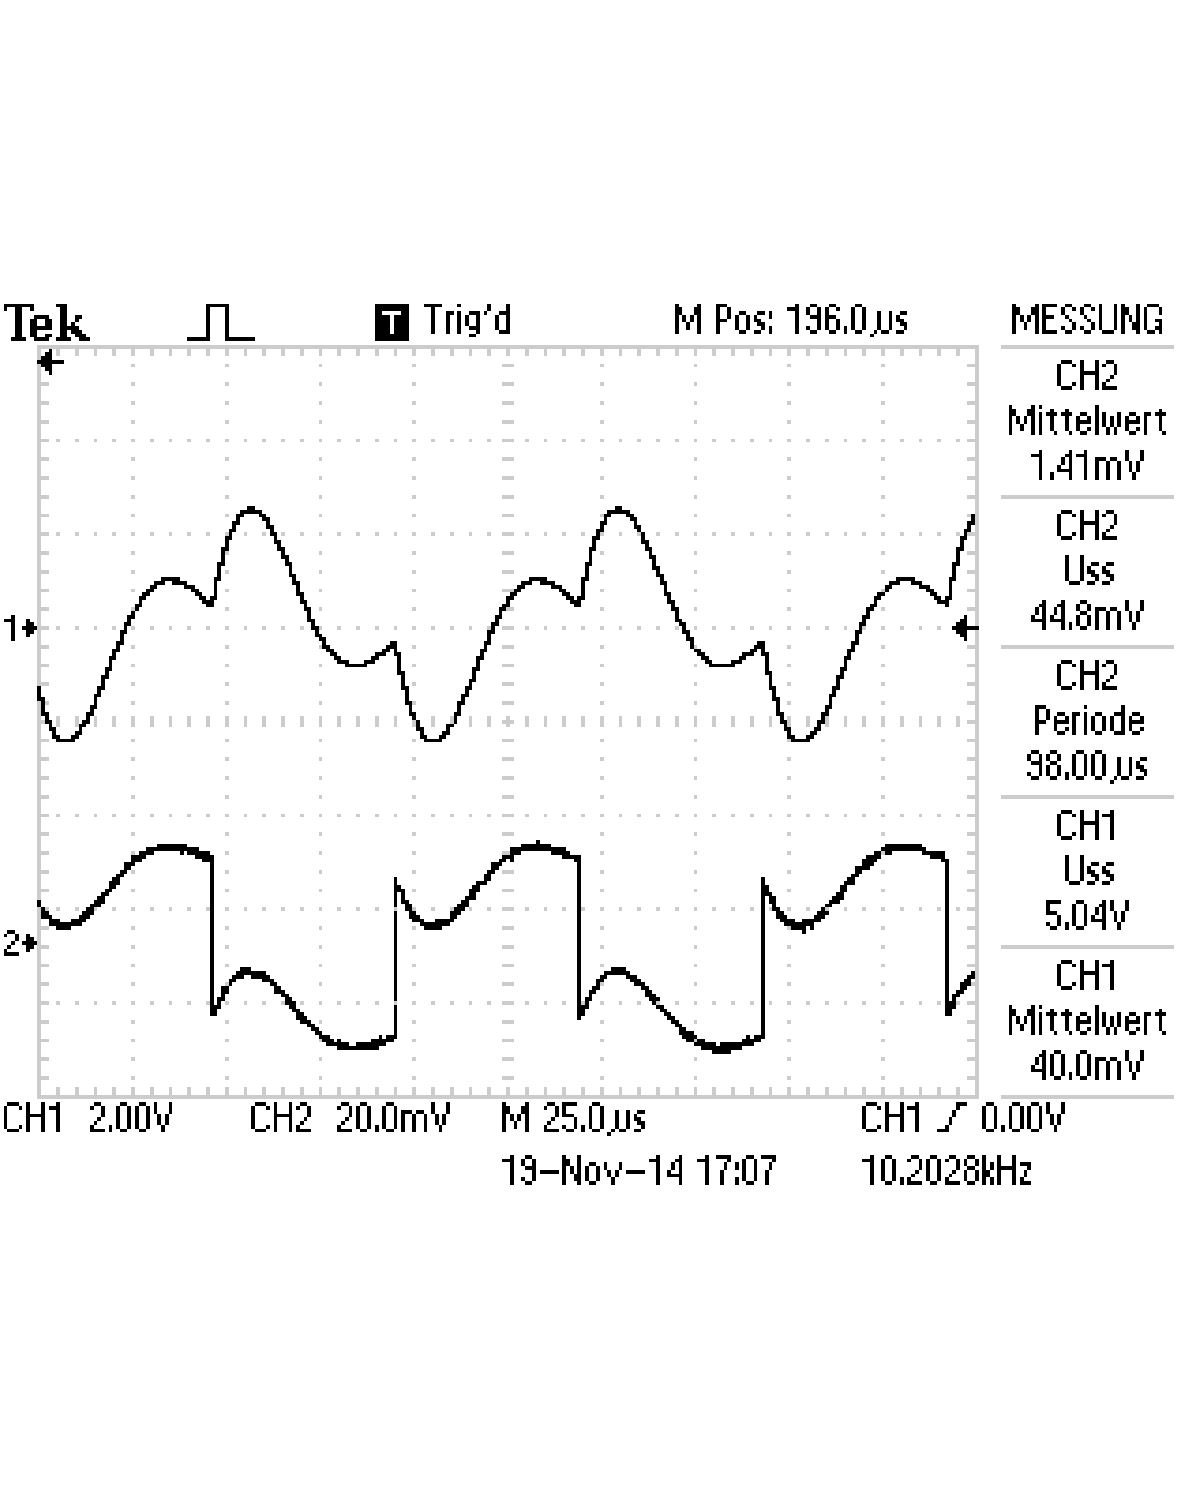
\includegraphics[width=\textwidth , scale = 0.4]{2_5_recht_10k.pdf}
                \caption[Aufnahme des Signals bei 10kHz]{Aufnahme des Signals bei 10kHz}
  				\label{fig:2_5_recht_10k}
        \end{subfigure}
        \caption{Kurven für 100Hz, 1kHz und 10kHz, bei einer Rechteckspannung}
        \label{fig:2_5_recht}
\end{figure}



\begin{figure}[H]
        \centering
        \begin{subfigure}[b]{0.28\textwidth}
                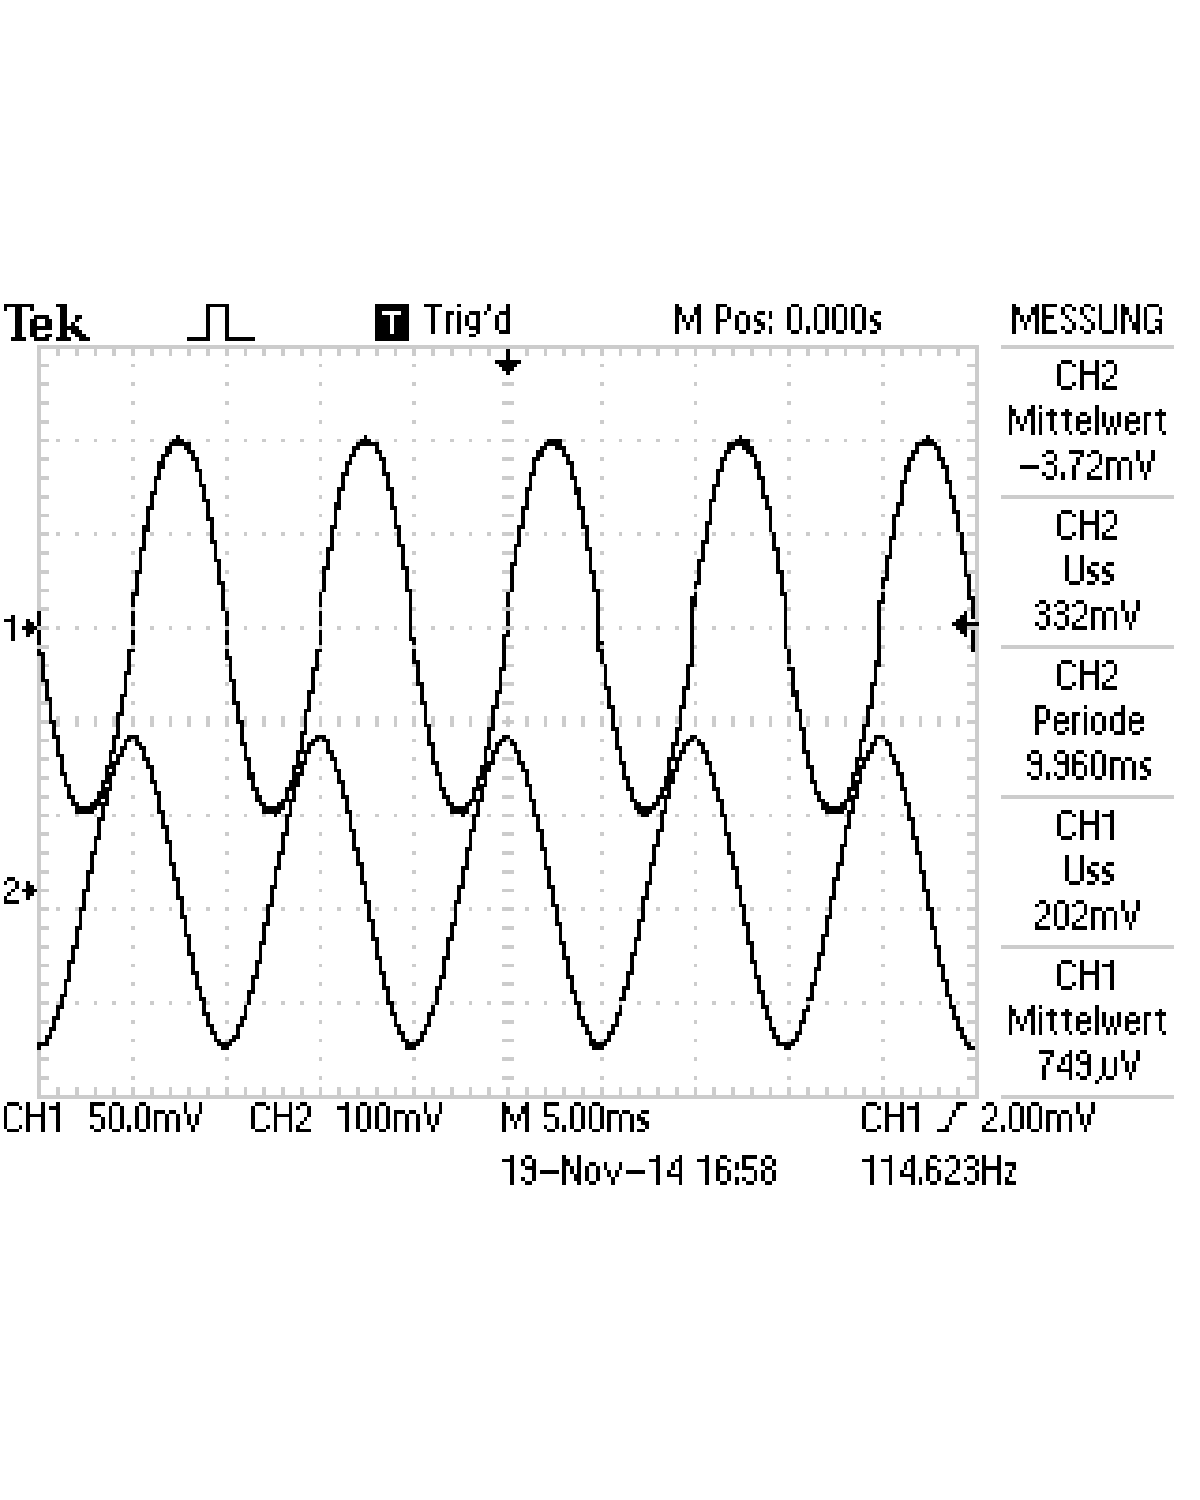
\includegraphics[width=\textwidth , scale = 0.4]{2_5_sin_100.pdf}
                \caption[Aufnahme des Signals bei 100Hz]{Aufnahme des Signals bei 100Hz}
                \label{fig:2_5_sin_100}
        \end{subfigure}%
       % ~ %add desired spacing between images, e. g. ~, \quad, \qquad, \hfill etc.
          %(or a blank line to force the subfigure onto a new line)
        \hfill
        \begin{subfigure}[b]{0.28\textwidth}
                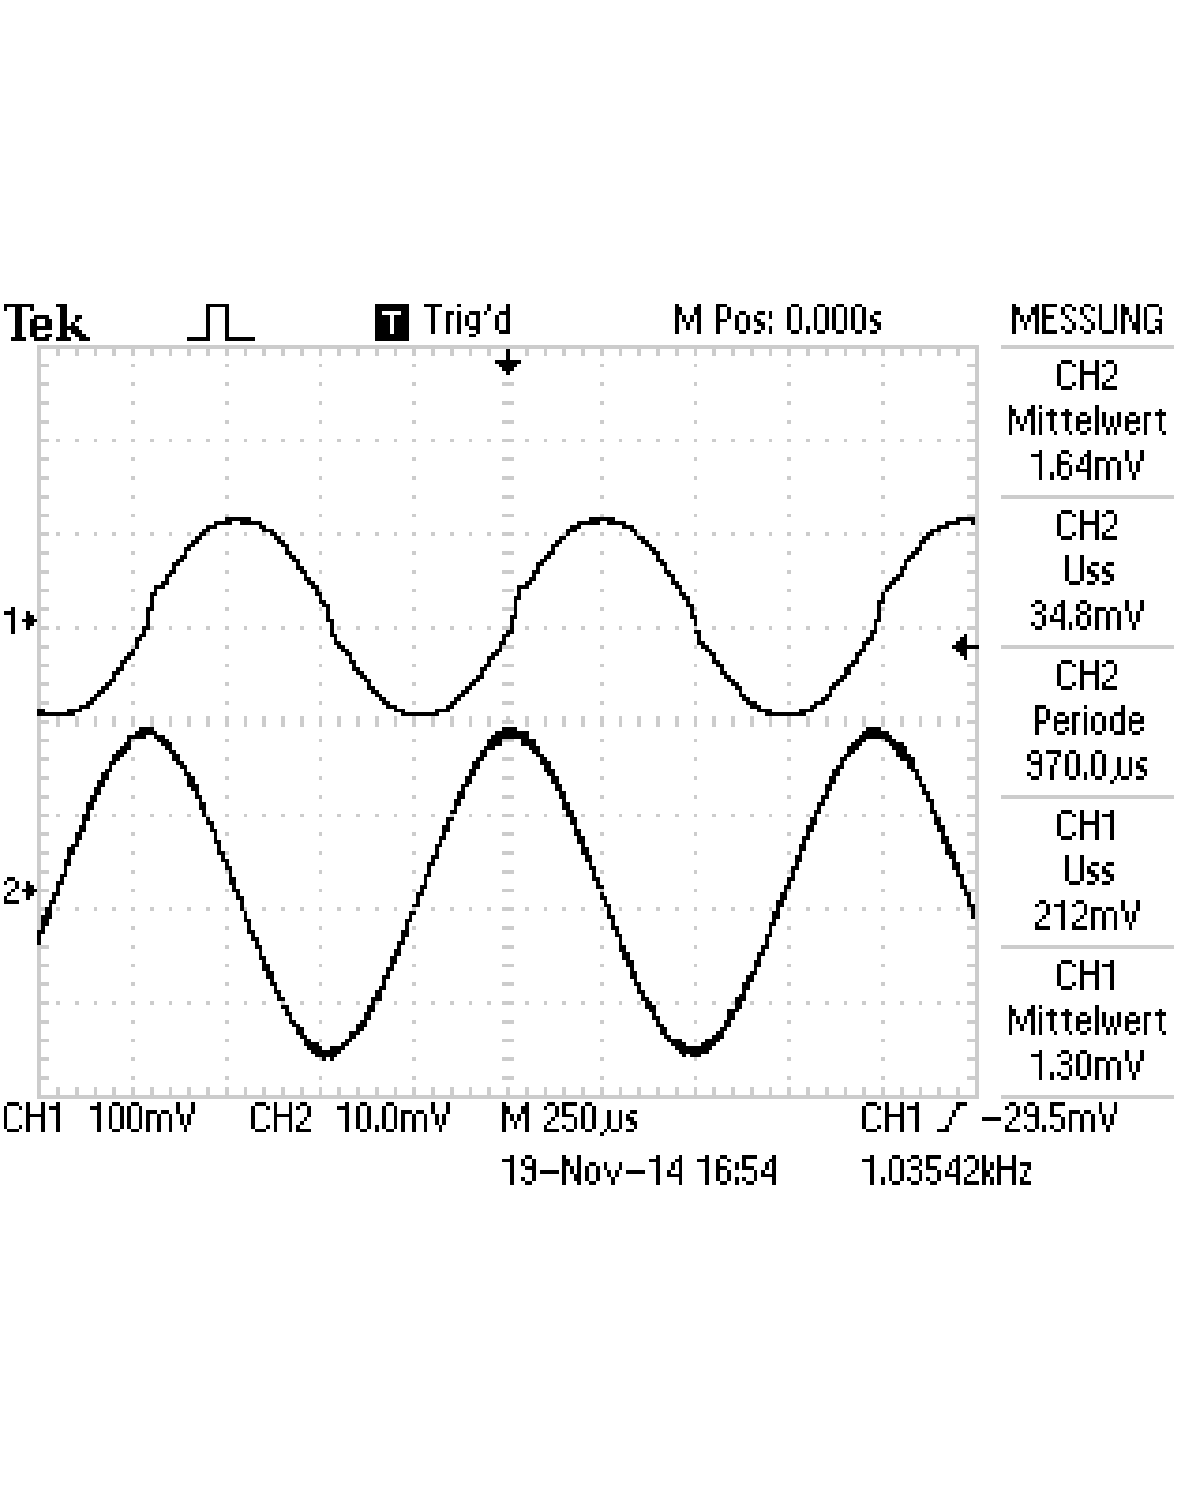
\includegraphics[width=\textwidth , scale = 0.4]{2_5_sin_1k.pdf}
                \caption[Aufnahme des Signals bei 1kHz]{Aufnahme des Signals bei 1kHz}
                \label{fig:2_5_sin_1k}
        \end{subfigure}
       % ~ %add desired spacing between images, e. g. ~, \quad, \qquad, \hfill etc.
          %(or a blank line to force the subfigure onto a new line)
        \hfill
        \begin{subfigure}[b]{0.28\textwidth}
                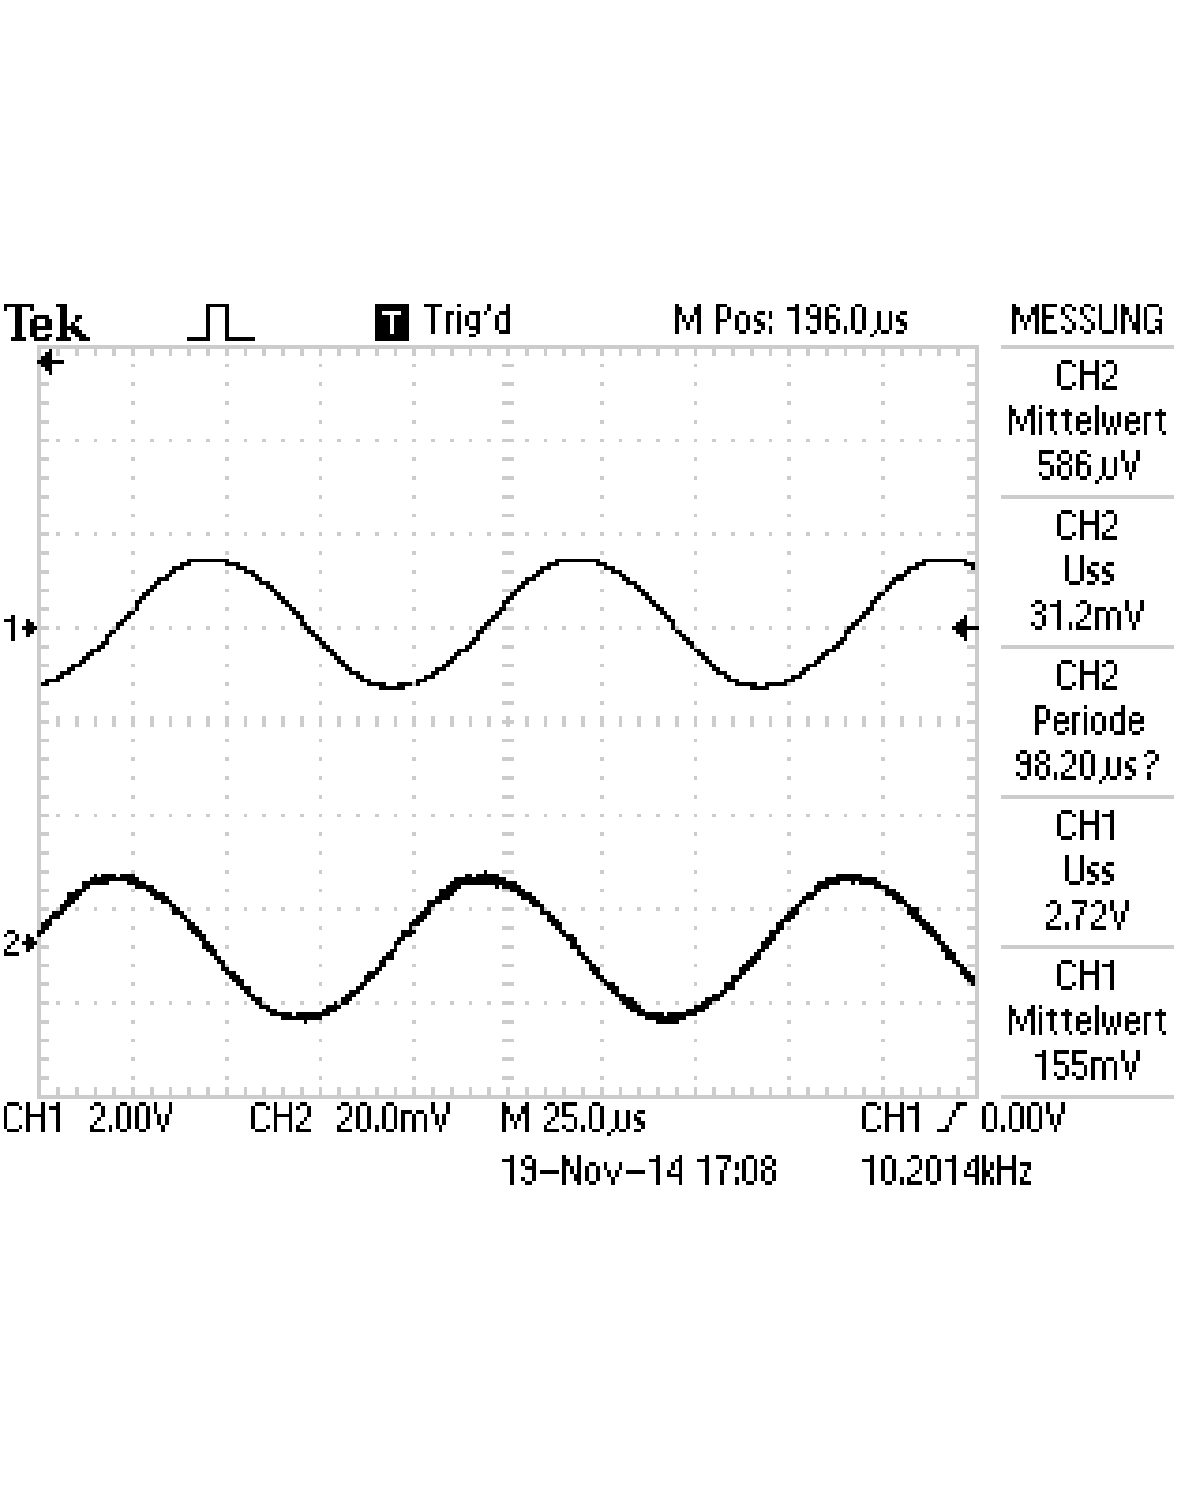
\includegraphics[width=\textwidth , scale = 0.4]{2_5_sin_10k.pdf}
                \caption[Aufnahme des Signals bei 10kHz]{Aufnahme des Signals bei 10kHz}
  				\label{fig:2_5_sin_10k}
        \end{subfigure}
        \caption{Kurven für 100Hz, 1kHz und 10kHz, bei einer Sinusspannung}
        \label{fig:2_5_sin}
\end{figure}


\subsection{Diskussion}
%(immer) die gemessenen werte und die bestimmten werte über die messfehler mit literaturwerten oder untereinander vergleichen
%in welchem fehlerintervall des messwertes liegt der literaturwert oder der vergleichswert?
%wie ist der relative anteil des fehlers am messwert und damit die qualität unserer messung?
%in einem satz erklären, wie gut unser fehler und damit unsere messung ist
%kurz erläutern, wie systematische fehler unsere messung beeinflusst haben könnten
%(wichtig) zum schluss ansprechen, in wie weit die ergebnisse mit der theoretischen vorhersage übereinstimmen
%--------------------------------------------------------------------------------------------
%falls tabellen mit den messwerten zu lang werden, kann die section mit den messwerten auch hinter der diskussion angefügt bzw. eine section mit dem anhang eingefügt werden.
%1-----------------------------------------------1

Die Eigenschaft als Differenzierer des Op-Amp konnte für kleine Frequenzen gut gezeigt werden, besonders gut lies sich der Effekt bei der Dreiecksspannung sehen. Für große Frequenzen treten wie erwartet Störungen auf.

\section{Integrierer}
%kurz das ziel dieses versuchsteiles ansprechen, damit keine zwei überschriften direkt übereinander stehen!
%bei schwierigeren versuchen kann auch der theoretische hintergrund erläutert werden. (mit formeln, herleitungen und erklärungen)
Mit der Schaltung in diesem Versuchsteil kann das Eingangssignal Integriert werden.
\subsection{Verwendete Geräte}
%(immer) eine skizze oder ein foto einfügen, die geräte/materialien !nummerieren! und z.b. eine legende dazu schreiben, besser wäre es das ganze in einem Fließtext gut zu beschreiben.
%falls am anfang des versuches nicht klar ist, was alles verwendet wird, wenn möglich erst am ende ein großes foto von den verwendeten materialien machen!\\

Für die Messung werden ein Kondensator, ein Widerstand, ein Operationsverstärker, ein Funktionsgenerator und DVMs verwendet.

\subsection{Verwendete Formeln}
%eine legende kann angefertigt werden, die selbstverständlichen buchstaben müssen nicht extra erklärt werden
%mit knappen erklärungen die !verwendeten! formeln, sowie die zugehörige fehlerrechnung einfügen
%2-----------------------------------------------2
Mit der Formel
\begin{align}
U_a = -\frac{1}{C_fR_i}\int U_idt
\end{align}
welche sich aus der Knotenregel und der Definition der Kapazität ergibt, kann die Ausgangsspannung berechnet werden.
%ab hier kann nochmal in einzelne versuchsteile unterteilt werden
\subsection{Versuchsaufbau}
%skizze zum versuchsaufbau (oder foto) einfügen,   es muss erklärt werden wie das ganze funktioniert und welche speziellen einstellungen verwendet wurden (z.b. welche knöpfe an den geräten für die messung verdreht wurden)

C ist ein 0,1$\mu$F Kondensator, R ein 10k$\Omega$ Widerstand, FG sollte mit 500Hz betrieben werden.

\begin{figure}[H] 
  \centering
    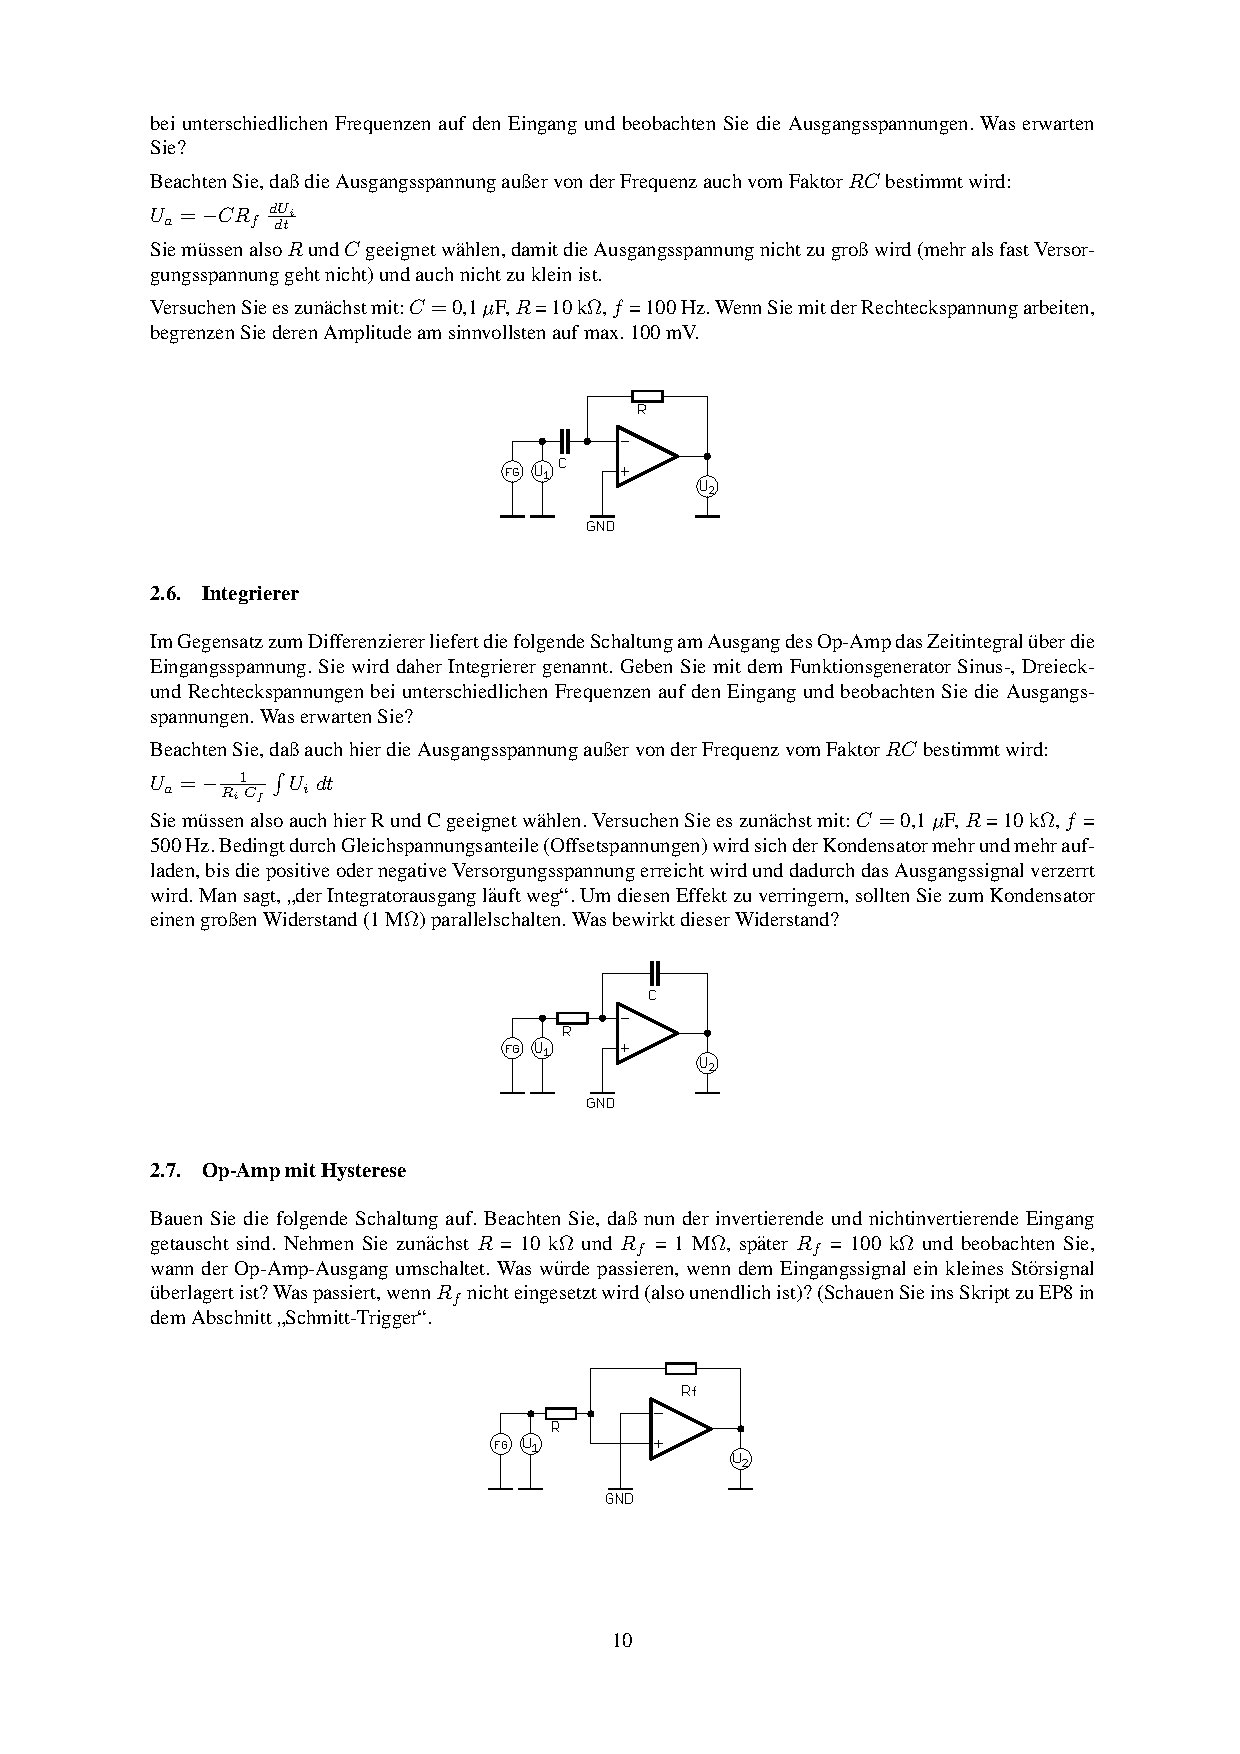
\includegraphics[trim = 10mm 105mm 10mm 160mm, clip, scale = 1]{ep4_14[Page10].pdf}
  	\caption[Schaltskizze des Integrierers]{Schaltskizze des Integrierers\footnotemark}
  \label{fig:1}
\end{figure}
\footnotetext{Abbildung entnommen von http://www.atlas.uni-wuppertal.de/$\sim$kind/ep4\_14.pdf Seite 10 am 17.11.2014}

\subsection{Versuchsdurchführung}
%erklären, !was! wir machen, !warum! wir das machen und mit welchem ziel
%(wichtig) präzize erklären, wie bei dem versuch vorgegangen und was gemacht wurde
Im Gegensatz zum Differenzierer kann die Eingangsspannung mit dieser Schaltung integriert werden, was die Bezeichnung 'Integrierer' begründet. Die Herleitung dieser Beziehung folgt aus der Definition der Kapazität und der Knotenregel. Angefangen bei \unit[500]{Hz} werden bei Sinus-,Dreieck- und Rechteckspannung die Frequenzen durchgefahren und mit dem Oszilloskop aufgezeichnet. Ein zum Kondensator parallel geschalteter Widerstand soll verhindern, dass der Kondensator durch die Gleichspannungsanteile aufgelanden wird.

\subsection{Auswertung}
%zuerst !alle! errechneten werte entweder in ganzen sätzen aufzählen, oder in tabellen (übersichtlicher) dargestellen, sowie auf die verwendeten formeln verweisen (die referenzierung der formel kann in der überschrift stehen)
%kurz erwähnen (vor der tabelle), warum wir das ganze ausrechnen bzw. was wir dort ausrechnen
%danach histogramme und plots erstellen, wobei wenn möglich funktionen durch die plots gelegt werden (zur not können auch splines benutzt werden, was aber angegeben werden muss)
%bei fits immer die funktion und das reduzierte chiquadrat mit angegeben, wobei auf verständlichkeit beim entziffern der zehnerpotenzen geachtet werden muss z.b. f(x)=(wert+-fehler)\cdot10^{irgendeine zahl}\cdot x + (wert+-fehler)\cdot10^{irgendeine zahl}
%bei jedem fit erklären, nach welchem zusammenhang gefittet wurde und warum!
%bei plots darauf achten, dass die achsenbeschriftung (auch die tics) die richtige größe haben und die legende im plot nicht die messwerte verdeckt
%kurz die aufgabenstellung abhandeln
%2-----------------------------------------------2

Im Versuchsteil 2.6 sollte die Eigenschaft des Integrierers untersucht werden. Dabei werden ein Dreieck-, Rechteck- und ein Sinussignal bei unterschiedlichen Frequenzen untersucht. Bei hohen Frequenzen ist ein Rauchen auf dem Ausgangssignal.  Bei niedrigen Frequenzen lässt sich vor allem bei der Rechteckspannung gut die Integration erkennen.

\begin{figure}[H]
        \centering
        \begin{subfigure}[b]{0.28\textwidth}
                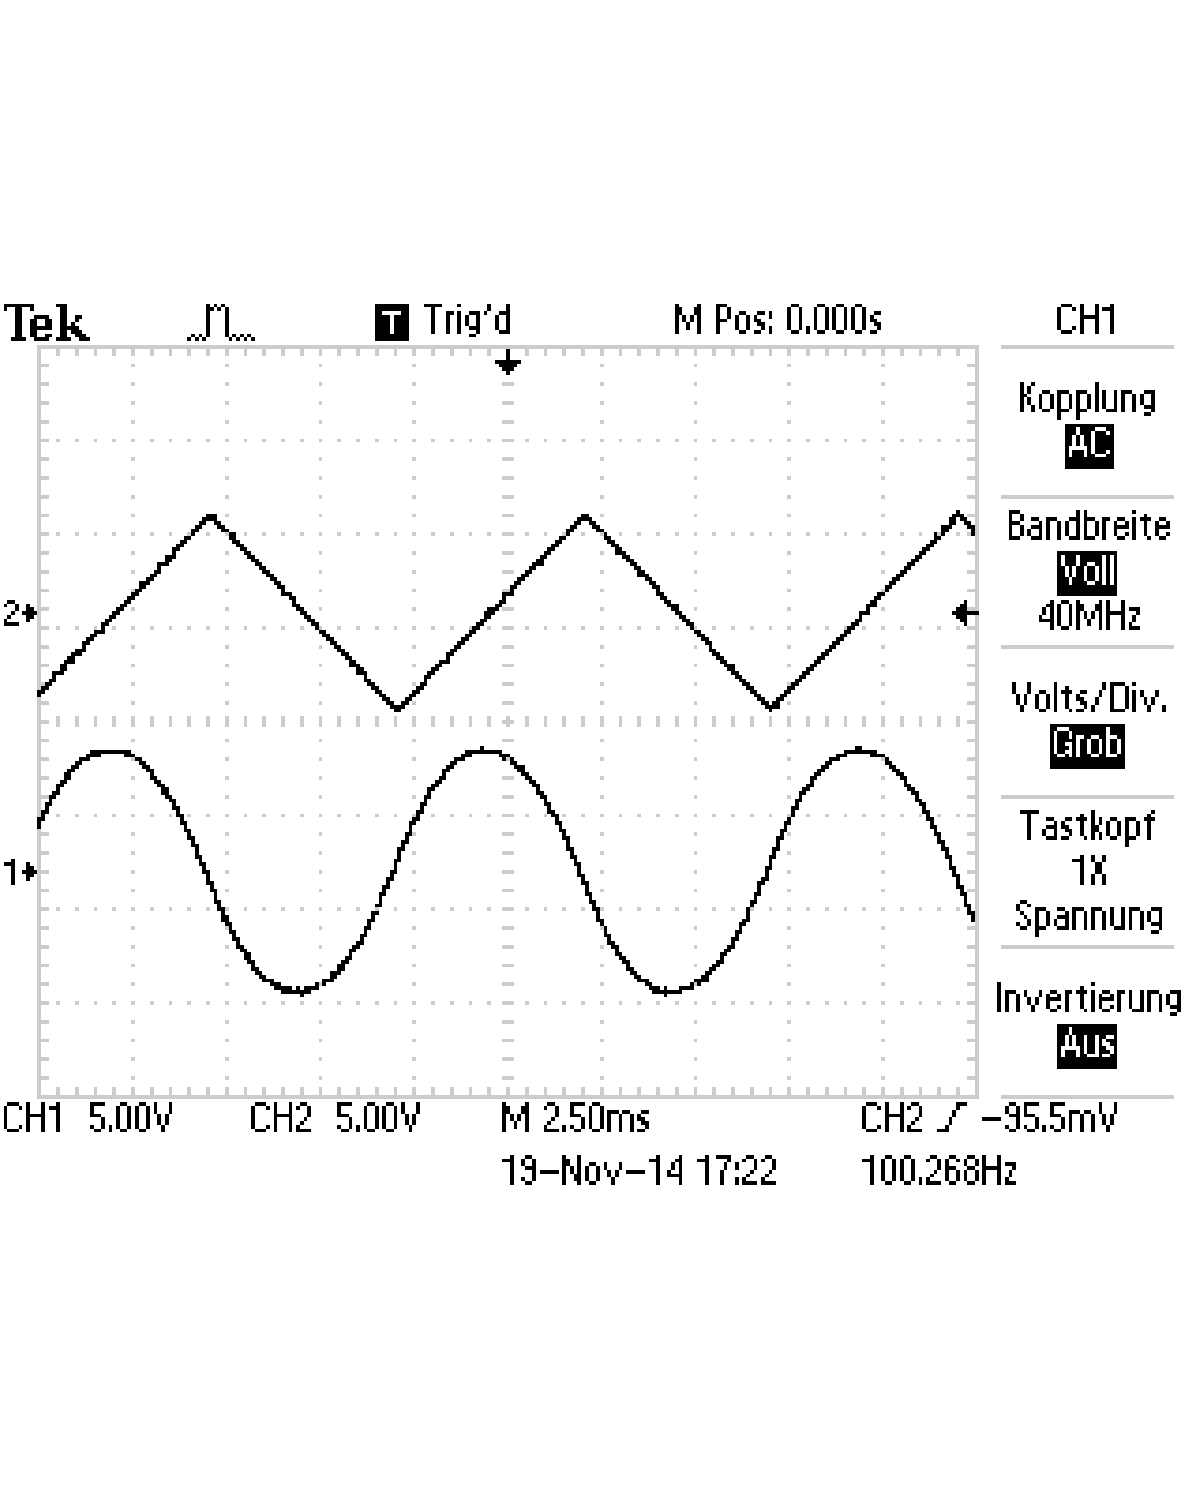
\includegraphics[width=\textwidth , scale = 0.4]{2_6_drei_100.pdf}
                \caption[Aufnahme des Signals bei 100Hz]{Aufnahme des Signals bei 100Hz}
                \label{fig:2_6_drei_100}
        \end{subfigure}%
       % ~ %add desired spacing between images, e. g. ~, \quad, \qquad, \hfill etc.
          %(or a blank line to force the subfigure onto a new line)
        \hfill
        \begin{subfigure}[b]{0.28\textwidth}
                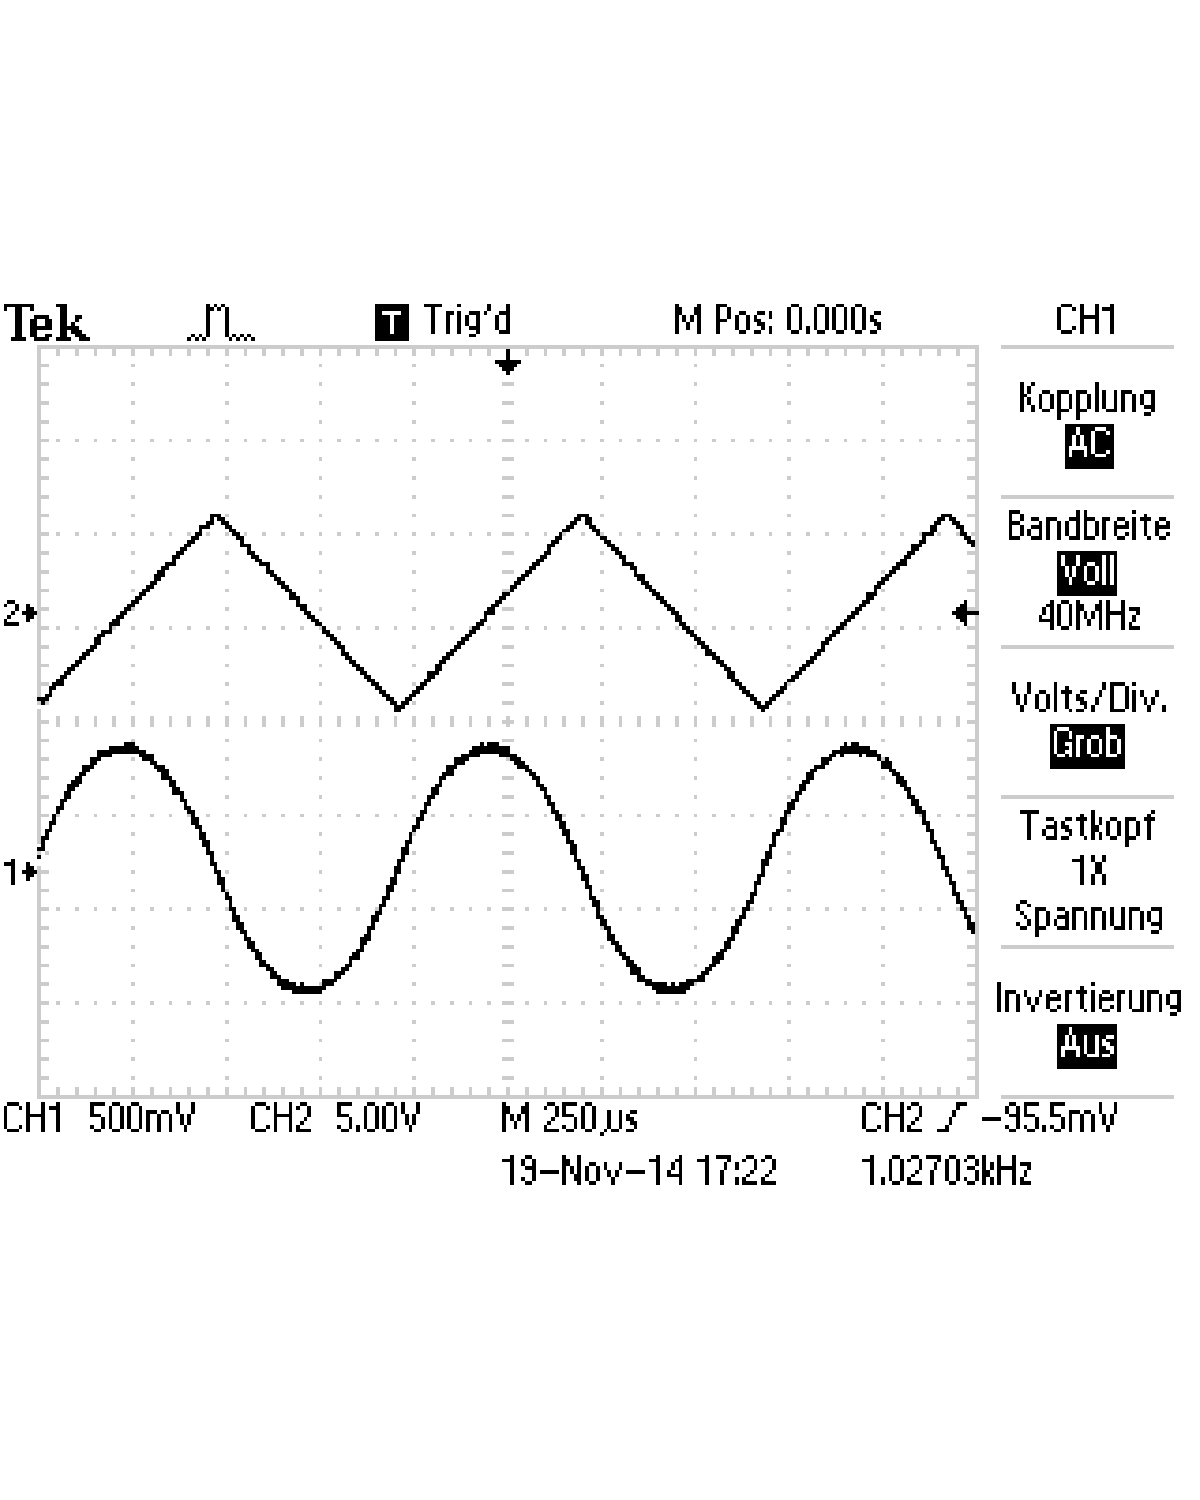
\includegraphics[width=\textwidth , scale = 0.4]{2_6_drei_1k.pdf}
                \caption[Aufnahme des Signals bei 1kHz]{Aufnahme des Signals bei 1kHz}
                \label{fig:2_6_drei_1k}
        \end{subfigure}
       % ~ %add desired spacing between images, e. g. ~, \quad, \qquad, \hfill etc.
          %(or a blank line to force the subfigure onto a new line)
        \hfill
        \begin{subfigure}[b]{0.28\textwidth}
                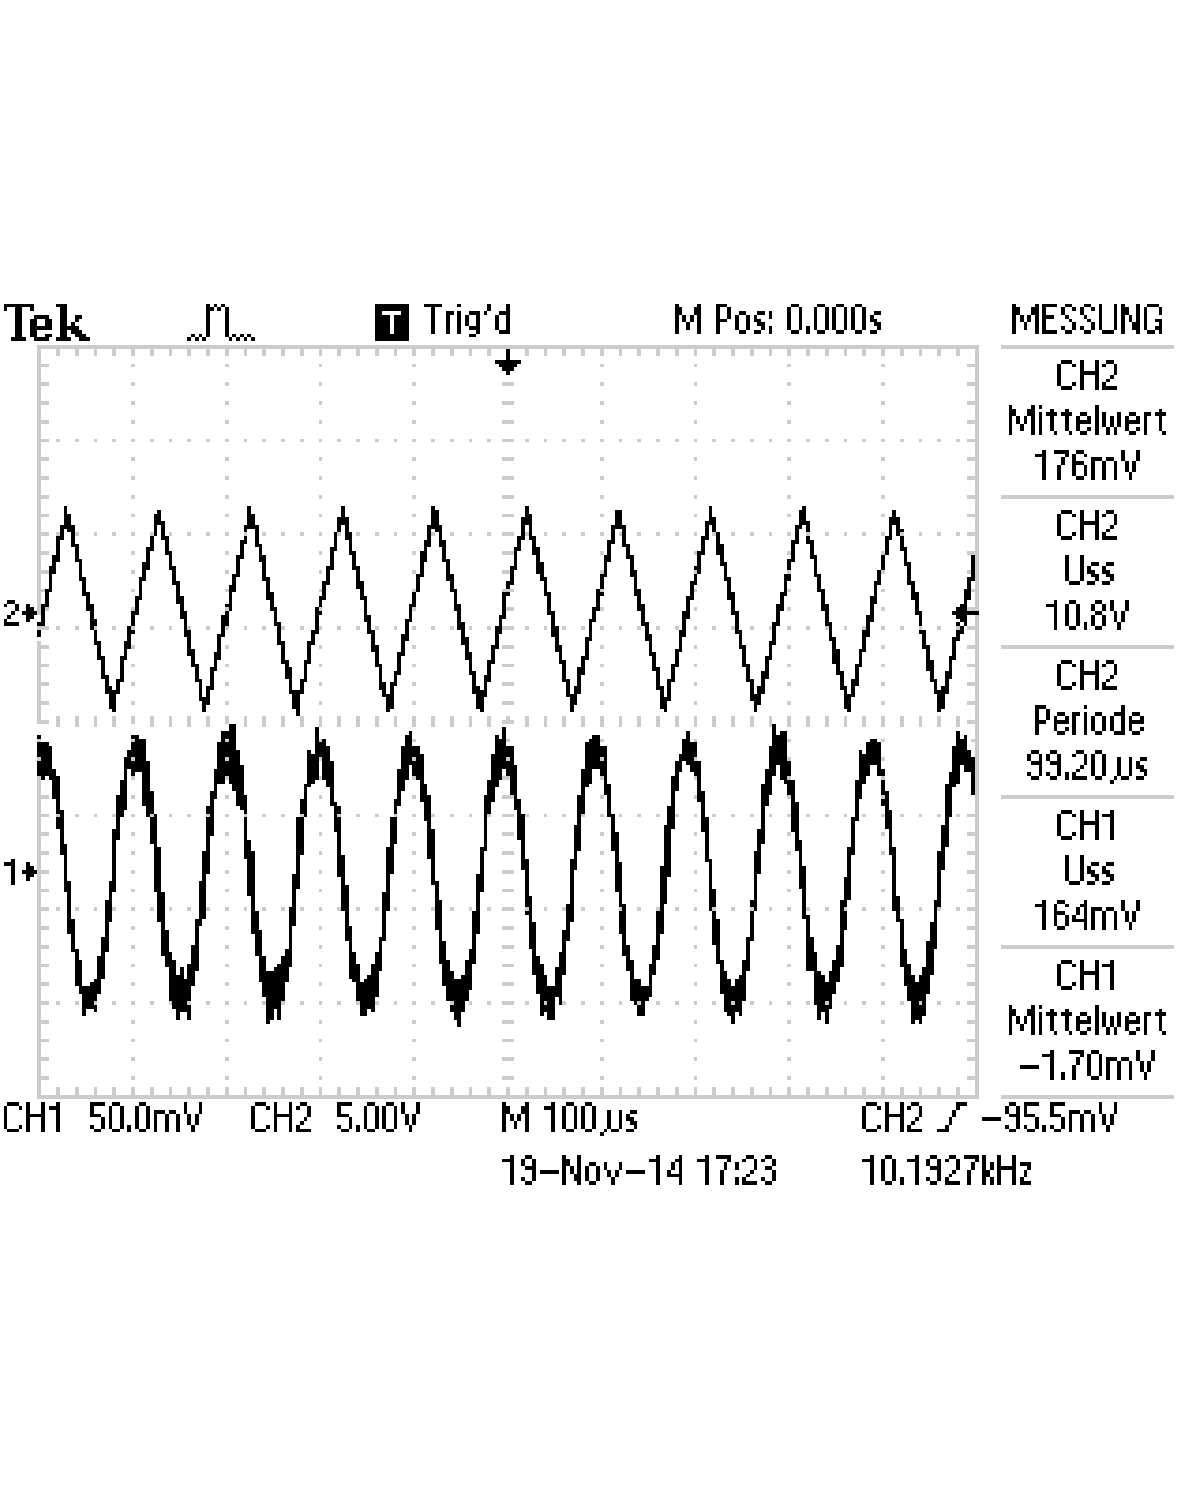
\includegraphics[width=\textwidth , scale = 0.4]{2_6_drei_10k.pdf}
                \caption[Aufnahme des Signals bei 10kHz]{Aufnahme des Signals bei 10kHz}
  				\label{fig:2_6_drei_10k}
        \end{subfigure}
        \caption{Kurven für 100Hz, 1kHz und 10kHz, bei einer Dreiecksspannung}
        \label{fig:2_6_drei}
\end{figure}




\begin{figure}[H]
        \centering
        \begin{subfigure}[b]{0.28\textwidth}
                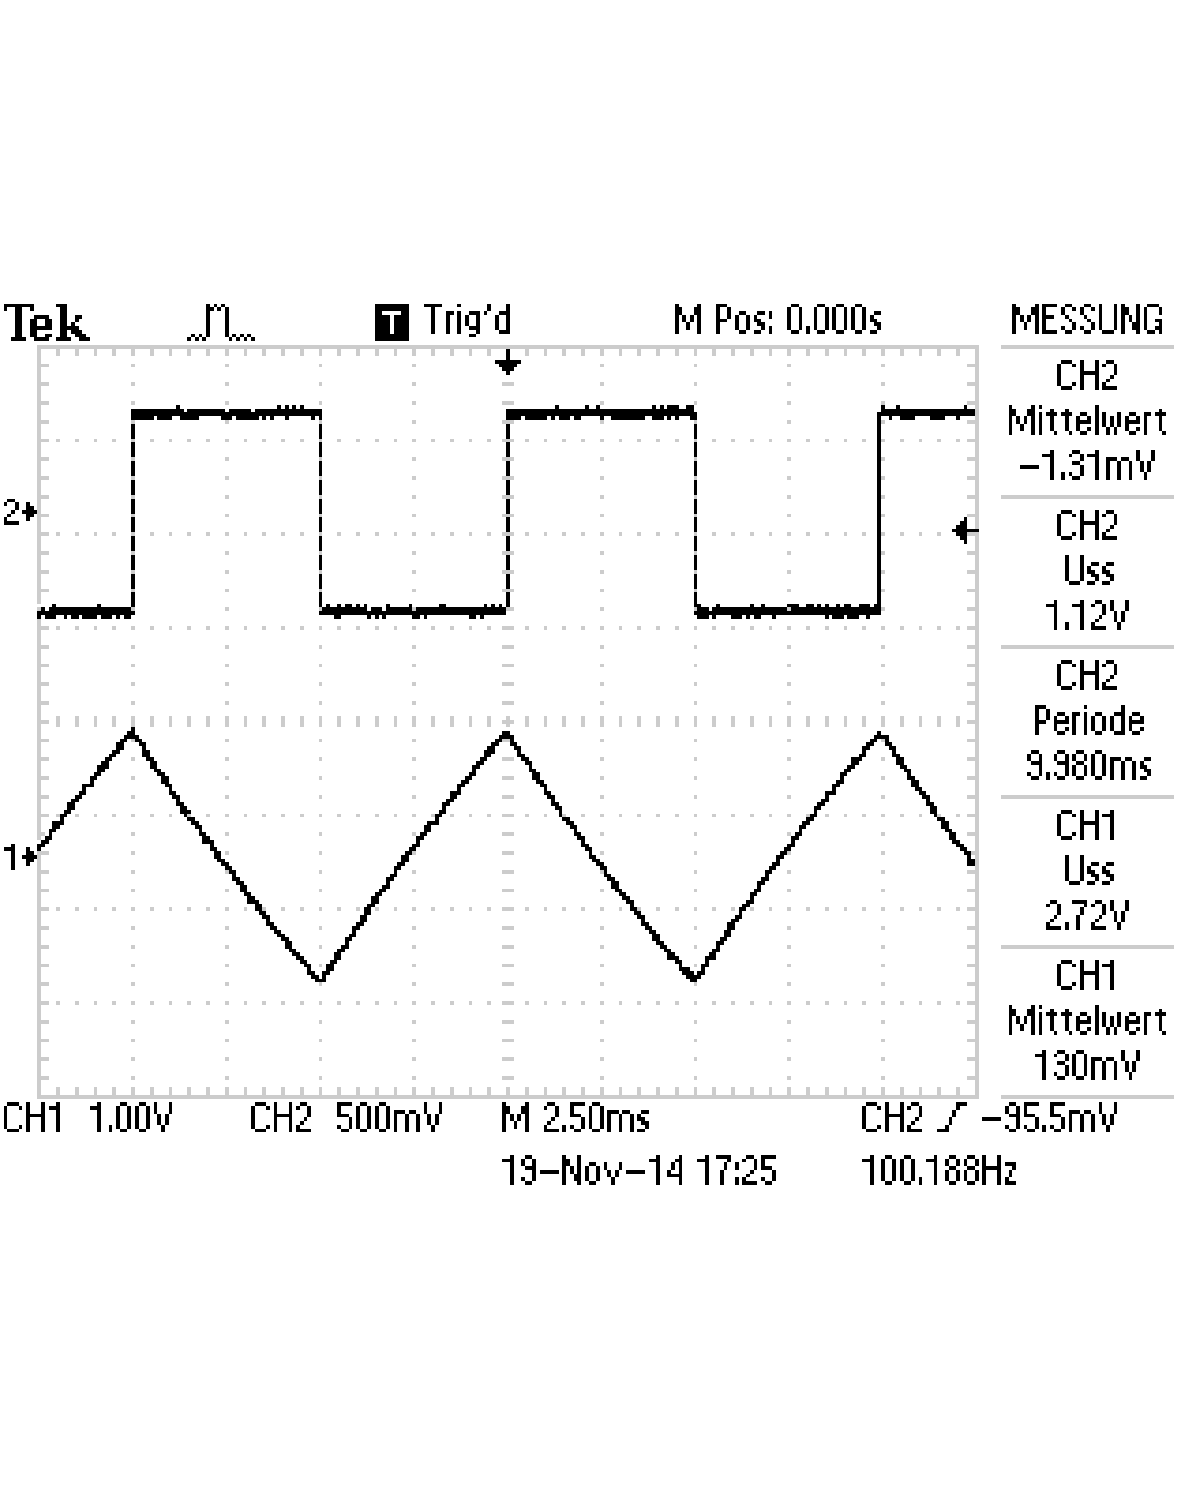
\includegraphics[width=\textwidth , scale = 0.4]{2_6_recht_100.pdf}
                \caption[Aufnahme des Signals bei 100Hz]{Aufnahme des Signals bei 100Hz}
                \label{fig:2_6_recht_100}
        \end{subfigure}%
       % ~ %add desired spacing between images, e. g. ~, \quad, \qquad, \hfill etc.
          %(or a blank line to force the subfigure onto a new line)
        \hfill
        \begin{subfigure}[b]{0.28\textwidth}
                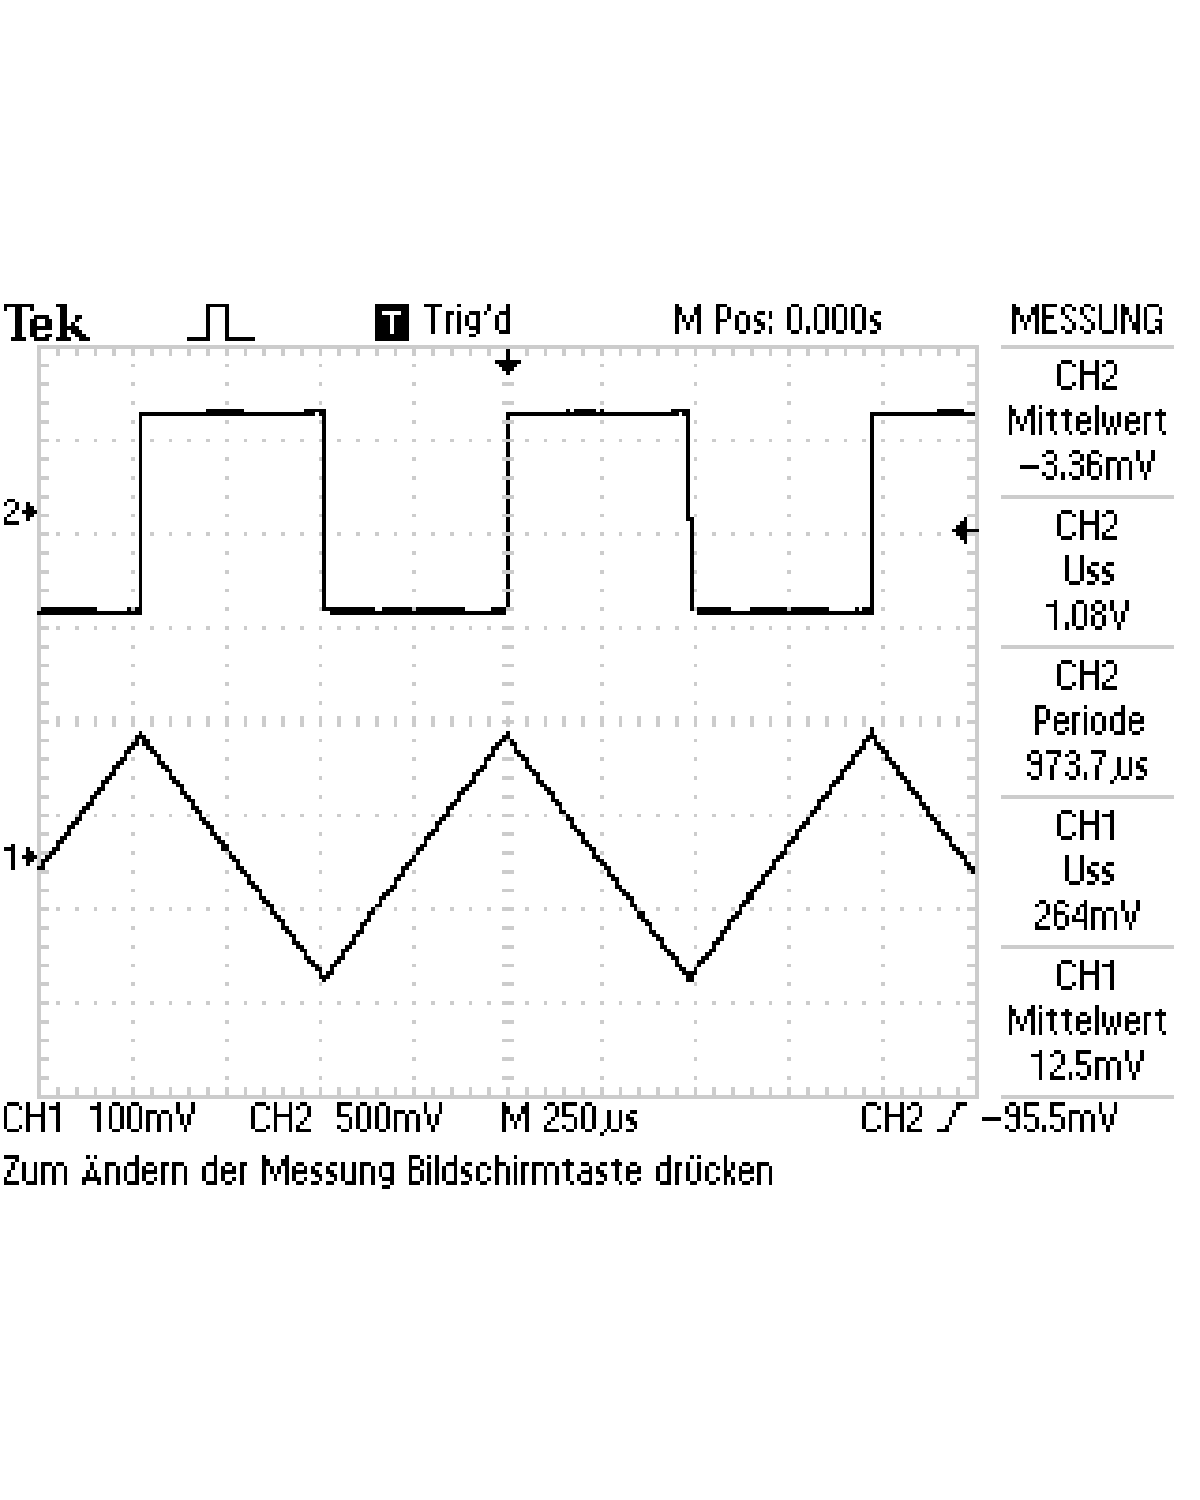
\includegraphics[width=\textwidth , scale = 0.4]{2_6_recht_1k.pdf}
                \caption[Aufnahme des Signals bei 1kHz]{Aufnahme des Signals bei 1kHz}
                \label{fig:2_6_recht_1k}
        \end{subfigure}
       % ~ %add desired spacing between images, e. g. ~, \quad, \qquad, \hfill etc.
          %(or a blank line to force the subfigure onto a new line)
        \hfill
        \begin{subfigure}[b]{0.28\textwidth}
                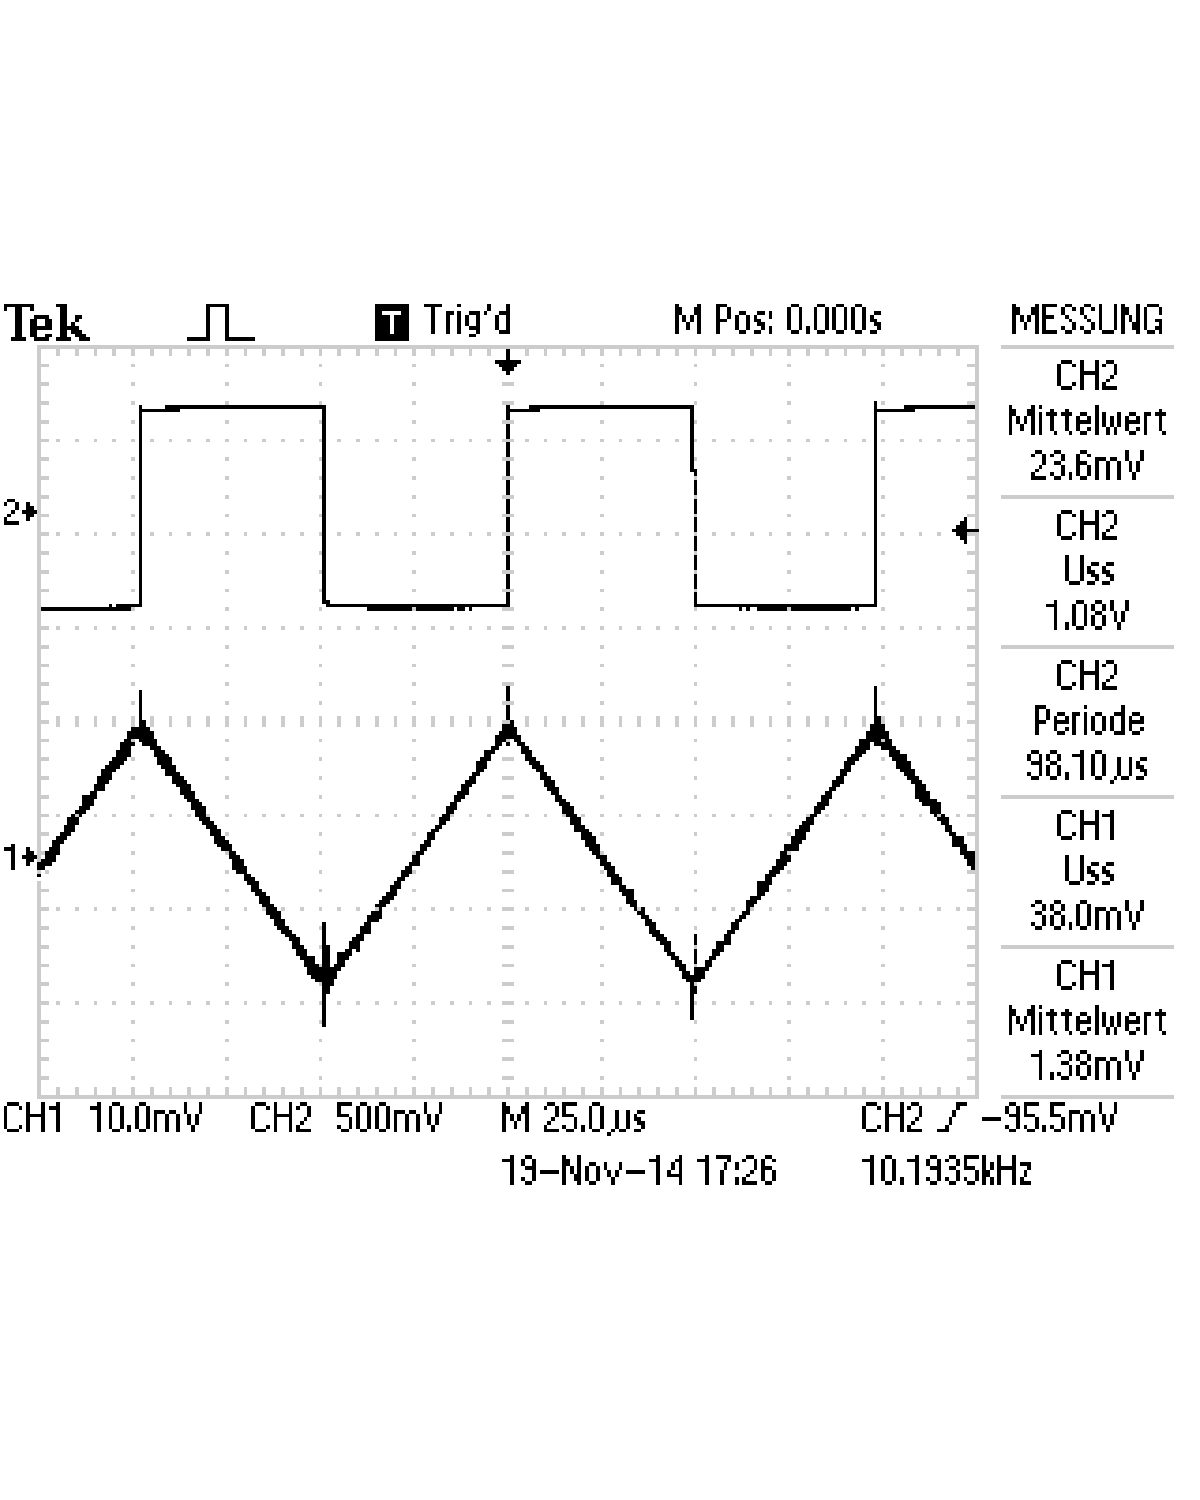
\includegraphics[width=\textwidth , scale = 0.4]{2_6_recht_10k.pdf}
                \caption[Aufnahme des Signals bei 10kHz]{Aufnahme des Signals bei 10kHz}
  				\label{fig:2_6_recht_10k}
        \end{subfigure}
        \caption{Kurven für 100Hz, 1kHz und 10kHz, bei einer Rechteckspannung}
        \label{fig:2_6_recht}
\end{figure}



\begin{figure}[H]
        \centering
        \begin{subfigure}[b]{0.28\textwidth}
                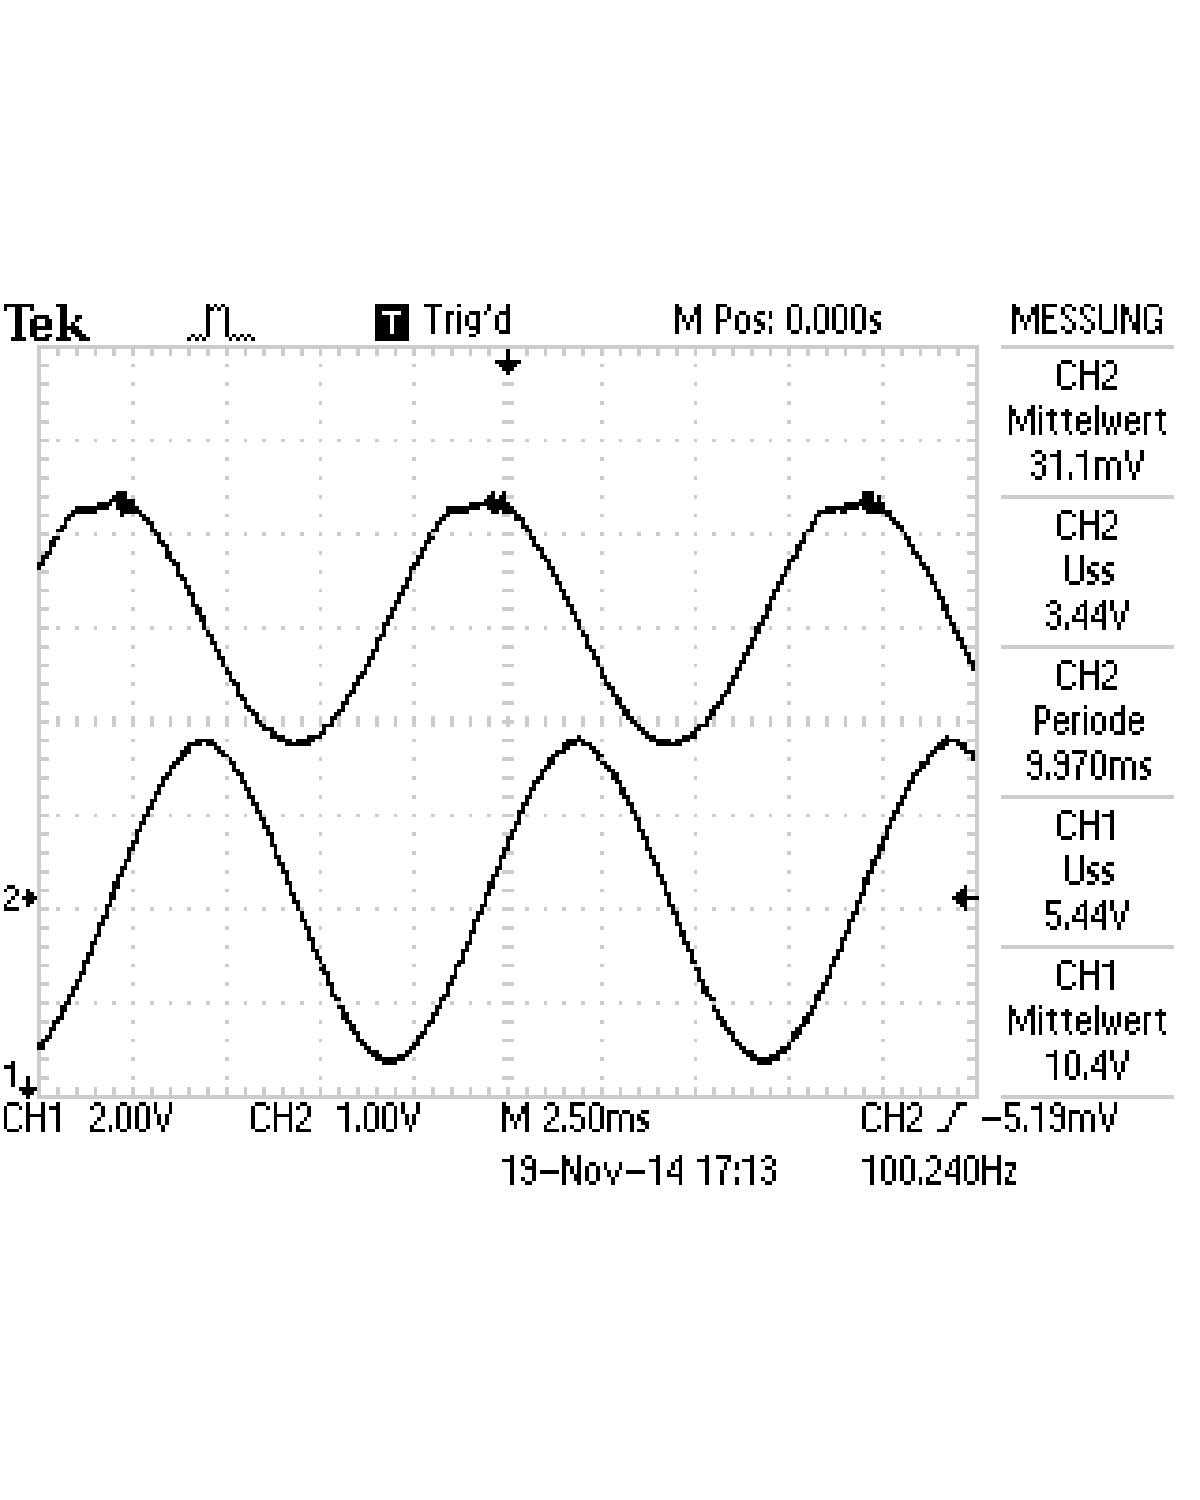
\includegraphics[width=\textwidth , scale = 0.4]{2_6_sin_100.pdf}
                \caption[Aufnahme des Signals bei 100Hz]{Aufnahme des Signals bei 100Hz}
                \label{fig:2_6_sin_100}
        \end{subfigure}%
       % ~ %add desired spacing between images, e. g. ~, \quad, \qquad, \hfill etc.
          %(or a blank line to force the subfigure onto a new line)
        \hfill
        \begin{subfigure}[b]{0.28\textwidth}
                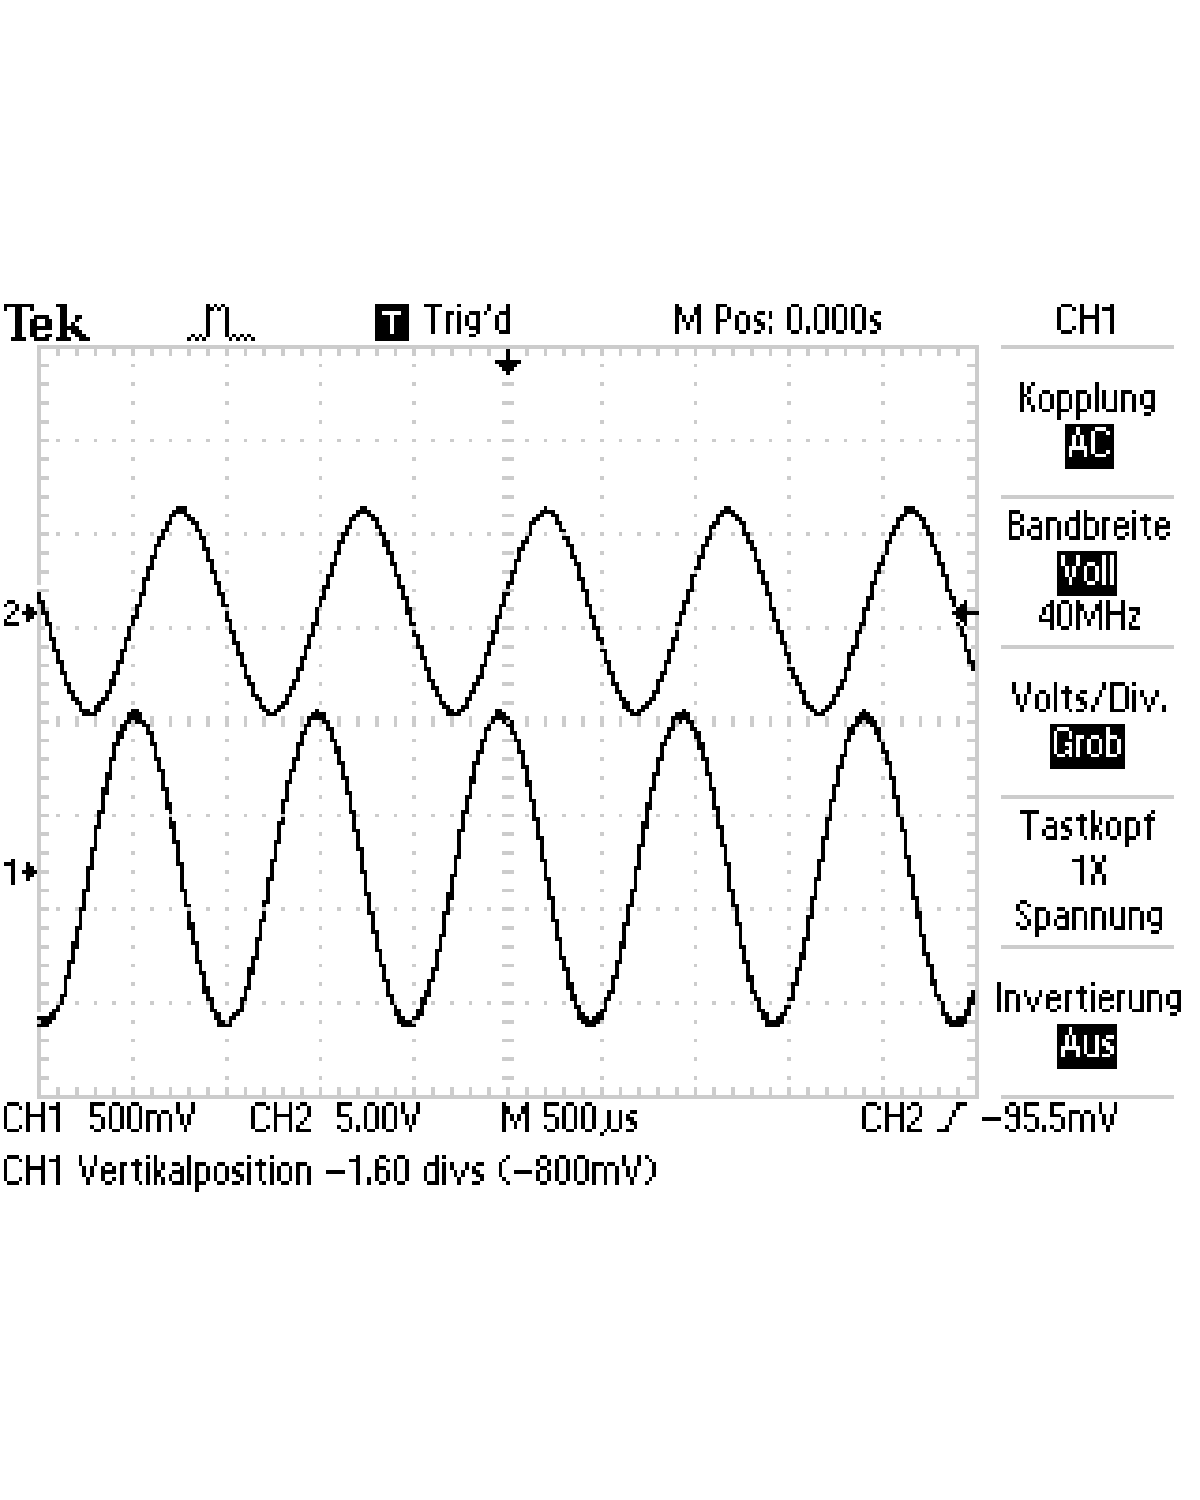
\includegraphics[width=\textwidth , scale = 0.4]{2_6_sin_1k.pdf}
                \caption[Aufnahme des Signals bei 1kHz]{Aufnahme des Signals bei 1kHz}
                \label{fig:2_6_sin_1k}
        \end{subfigure}
       % ~ %add desired spacing between images, e. g. ~, \quad, \qquad, \hfill etc.
          %(or a blank line to force the subfigure onto a new line)
        \hfill
        \begin{subfigure}[b]{0.28\textwidth}
                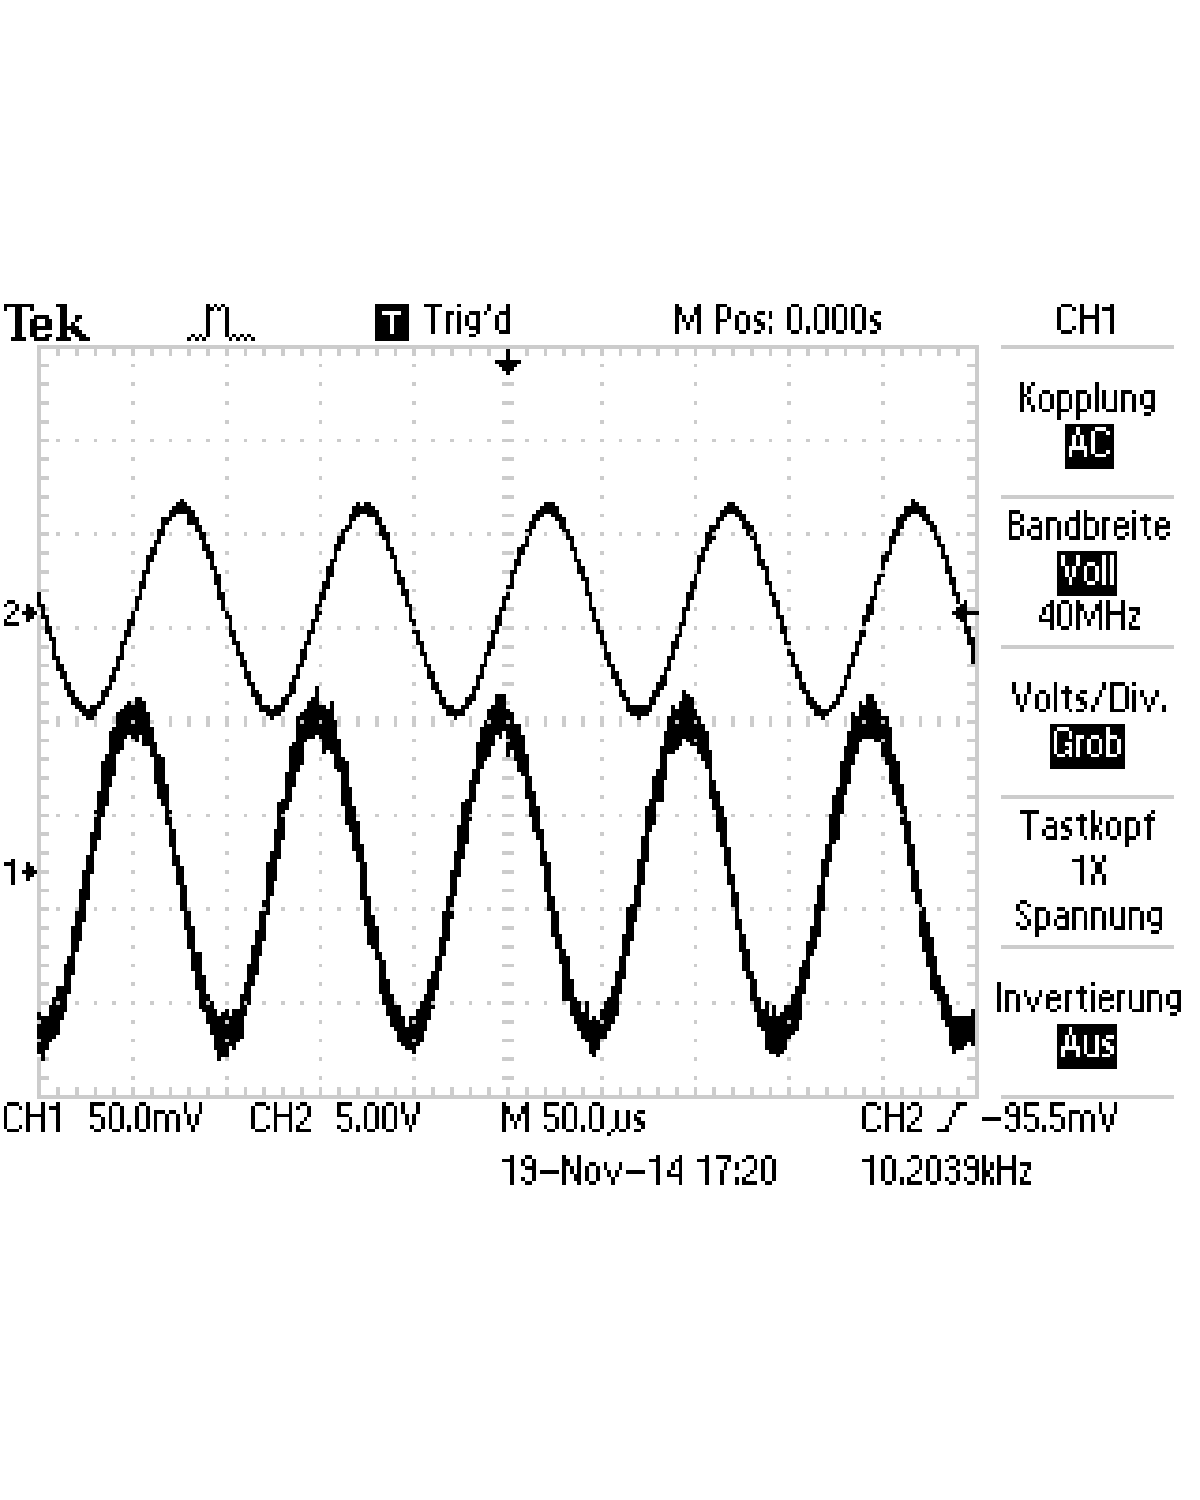
\includegraphics[width=\textwidth , scale = 0.4]{2_6_sin_10k.pdf}
                \caption[Aufnahme des Signals bei 10kHz]{Aufnahme des Signals bei 10kHz}
  				\label{fig:2_6_sin_10k}
        \end{subfigure}
        \caption{Kurven für 100Hz, 1kHz und 10kHz, bei einer Sinusspannung}
        \label{fig:2_6_sin}
\end{figure}

\subsection{Diskussion}
%(immer) die gemessenen werte und die bestimmten werte über die messfehler mit literaturwerten oder untereinander vergleichen
%in welchem fehlerintervall des messwertes liegt der literaturwert oder der vergleichswert?
%wie ist der relative anteil des fehlers am messwert und damit die qualität unserer messung?
%in einem satz erklären, wie gut unser fehler und damit unsere messung ist
%kurz erläutern, wie systematische fehler unsere messung beeinflusst haben könnten
%(wichtig) zum schluss ansprechen, in wie weit die ergebnisse mit der theoretischen vorhersage übereinstimmen
%--------------------------------------------------------------------------------------------
%falls tabellen mit den messwerten zu lang werden, kann die section mit den messwerten auch hinter der diskussion angefügt bzw. eine section mit dem anhang eingefügt werden.
%1-----------------------------------------------1

Die Eigenschaft als Integrator des Op-Amp konnte für kleine Frequenzen gut gezeigt werden, besonders gut lies sich der Effekt bei der Rechteckspannung sehen. Für große Frequenzen treten wie erwartet Störungen auf.

\section{Op-Amp mit Hysterese}
%kurz das ziel dieses versuchsteiles ansprechen, damit keine zwei überschriften direkt übereinander stehen!
%bei schwierigeren versuchen kann auch der theoretische hintergrund erläutert werden. (mit formeln, herleitungen und erklärungen)
Das Op-Amp soll rückgekoppelt werden, sodass Ausgangsspannung der Eingangsspannung zeitverzögert folgt. Dies liegt daran, dass das Op-Amp erst ab einer geringen "Umschaltspannung" dem Eingangssignal folgt.
\subsection{Verwendete Geräte}
%(immer) eine skizze oder ein foto einfügen, die geräte/materialien !nummerieren! und z.b. eine legende dazu schreiben, besser wäre es das ganze in einem Fließtext gut zu beschreiben.
%falls am anfang des versuches nicht klar ist, was alles verwendet wird, wenn möglich erst am ende ein großes foto von den verwendeten materialien machen!\\

Es werden Widerstände, ein Operationsverstärker und ein Funktionsgenerator verwendet.

\subsection{Versuchsaufbau}
%skizze zum versuchsaufbau (oder foto) einfügen,   es muss erklärt werden wie das ganze funktioniert und welche speziellen einstellungen verwendet wurden (z.b. welche knöpfe an den geräten für die messung verdreht wurden)

R ist ein 10k$\Omega$ Widerstand, Rf ein 1M$\Omega$ Widerstand, FG ist der Funktionsgenerator.

\begin{figure}[H] 
  \centering
    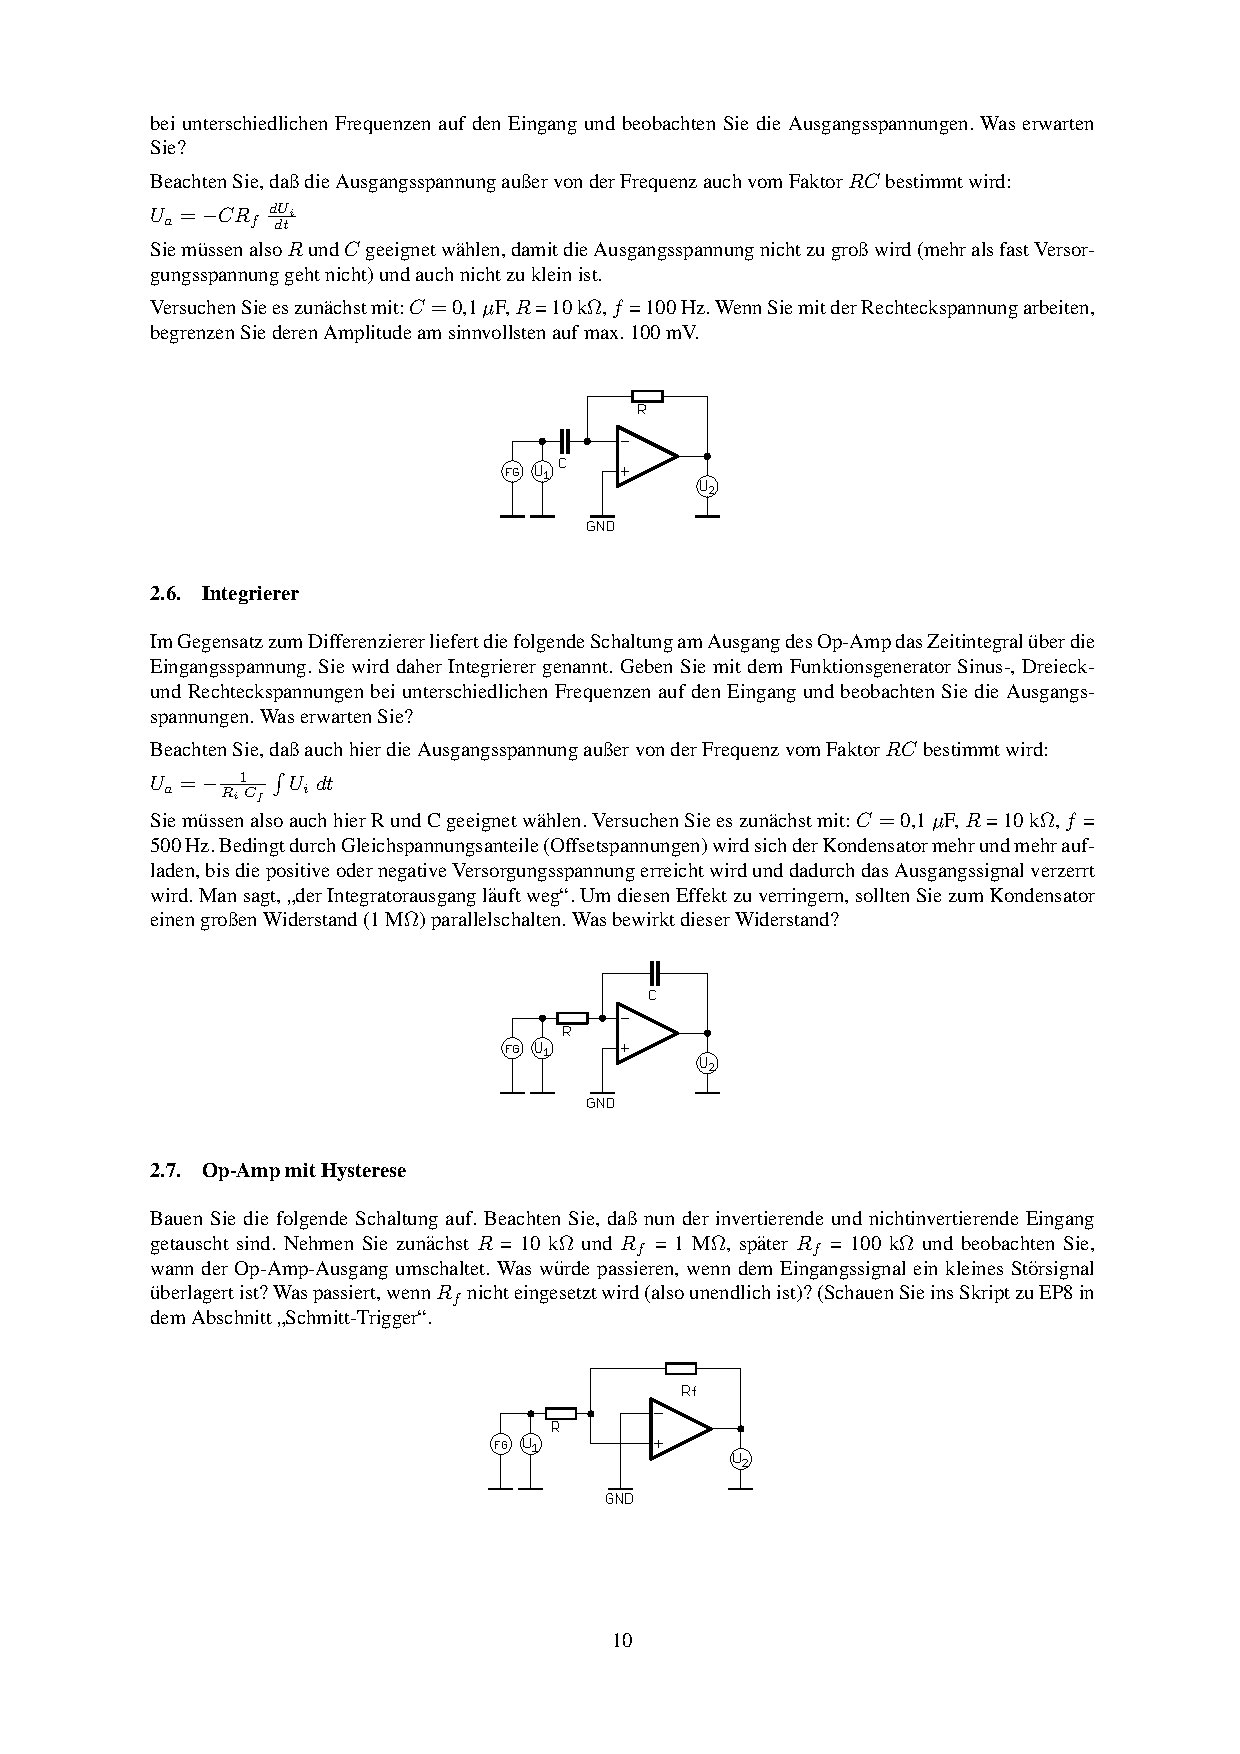
\includegraphics[trim = 10mm 40mm 10mm 230mm, clip, scale = 1]{ep4_14[Page10].pdf}
  	\caption[Schaltskizze des Op-Amp mit Hysterese]{Schaltskizze des Op-Amp mit Hysterese\footnotemark}
  \label{fig:1}
\end{figure}
\footnotetext{Abbildung entnommen von http://www.atlas.uni-wuppertal.de/$\sim$kind/ep4\_14.pdf Seite 10 am 17.11.2014}

\subsection{Versuchsdurchführung}
%erklären, !was! wir machen, !warum! wir das machen und mit welchem ziel
%(wichtig) präzize erklären, wie bei dem versuch vorgegangen und was gemacht wurde
In diesem Versuchsteil wird der Effekt der Hysterese mit Operationsverstärker über das Oszilloskop aufgenommen. Abhängig davon, ob der Ausgang des Operationsverstärkers über einen Widerstand rückgekoppelt wird, kann der Effekt beobachtet werden.

\subsection{Auswertung}
%zuerst !alle! errechneten werte entweder in ganzen sätzen aufzählen, oder in tabellen (übersichtlicher) dargestellen, sowie auf die verwendeten formeln verweisen (die referenzierung der formel kann in der überschrift stehen)
%kurz erwähnen (vor der tabelle), warum wir das ganze ausrechnen bzw. was wir dort ausrechnen
%danach histogramme und plots erstellen, wobei wenn möglich funktionen durch die plots gelegt werden (zur not können auch splines benutzt werden, was aber angegeben werden muss)
%bei fits immer die funktion und das reduzierte chiquadrat mit angegeben, wobei auf verständlichkeit beim entziffern der zehnerpotenzen geachtet werden muss z.b. f(x)=(wert+-fehler)\cdot10^{irgendeine zahl}\cdot x + (wert+-fehler)\cdot10^{irgendeine zahl}
%bei jedem fit erklären, nach welchem zusammenhang gefittet wurde und warum!
%bei plots darauf achten, dass die achsenbeschriftung (auch die tics) die richtige größe haben und die legende im plot nicht die messwerte verdeckt
%kurz die aufgabenstellung abhandeln
%2-----------------------------------------------2

In Versuchsteil 2.7 sollt der Effekt der Hysterese durch Rückkopplung des Op-Amp untersucht werden. In Abbildung \ref{fig:2_7_ohne_rf} ist der Verlauf des Signals ohne den Widerstand RF zu sehen. Betrachtet man Abbildung \ref{fig:2_7_mit_rf}, wo der Widerstand RF nicht weggelassen wurde, so ist deutlich der Effekt der Hysterese zu erkenne (Verschiebung des Rechtecksignals).

\begin{figure}[H]
        \centering
        \begin{subfigure}[b]{0.48\textwidth}
                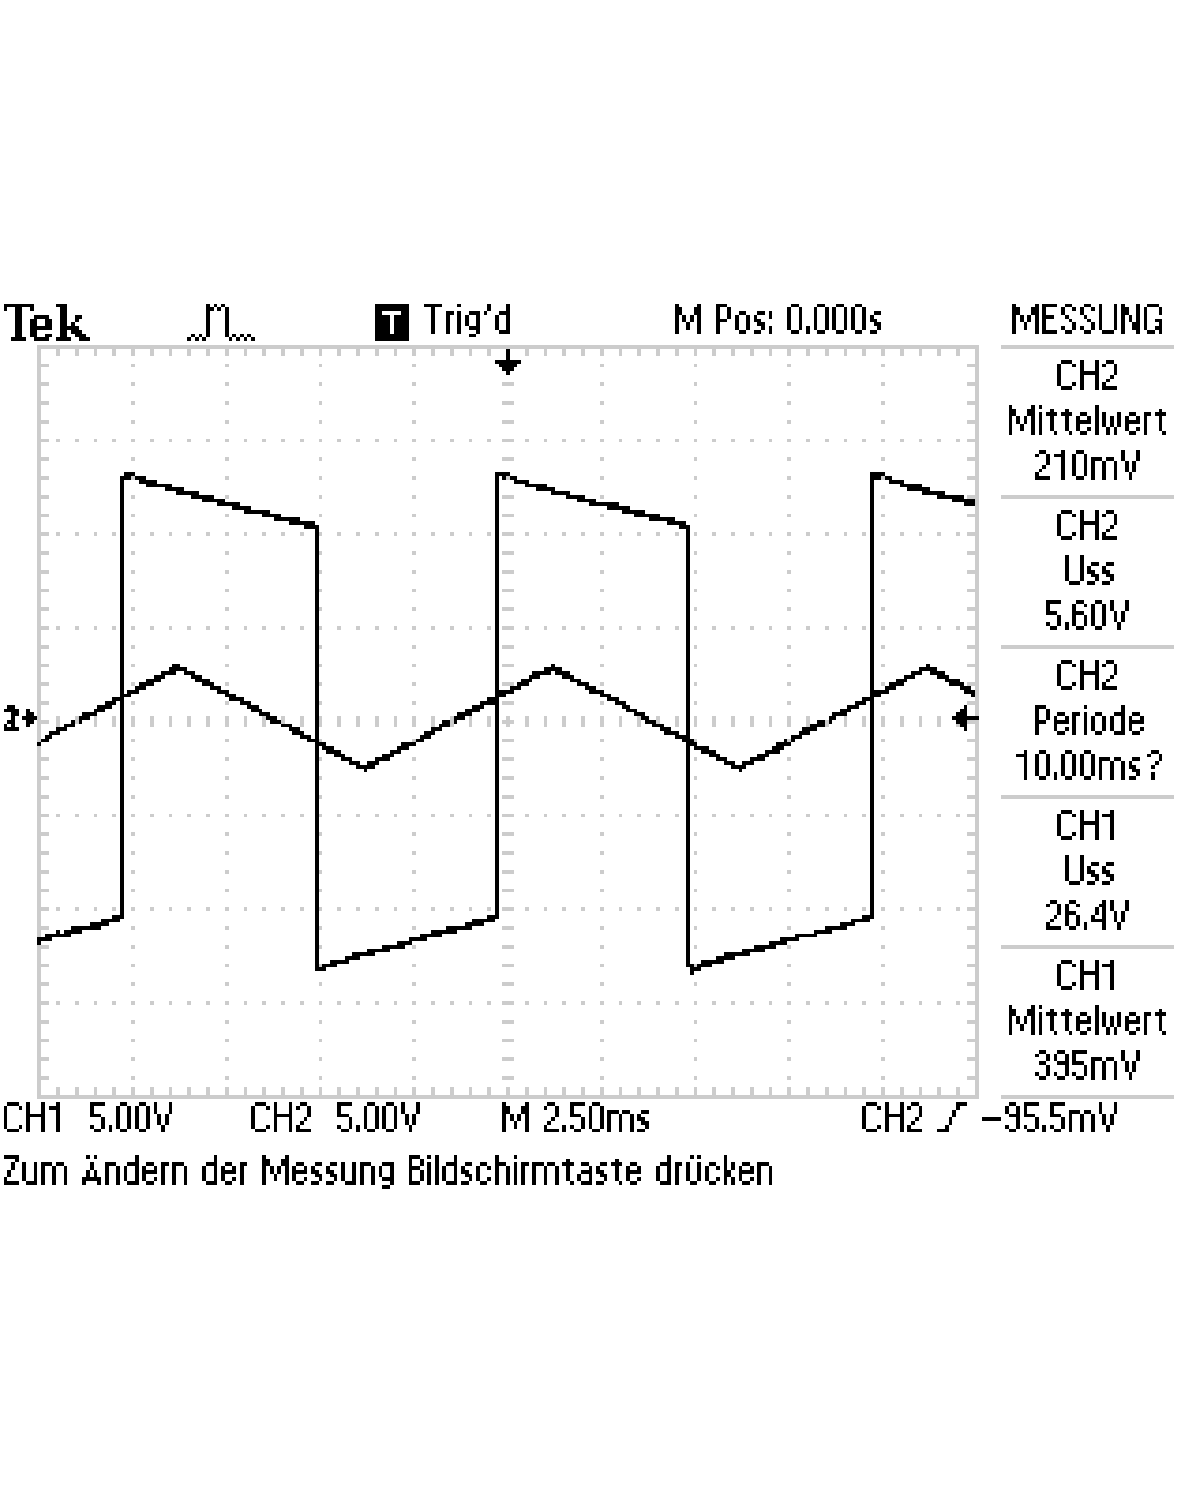
\includegraphics[width=\textwidth , scale = 0.4]{2_7_mit_rf.pdf}
                \caption[Aufnahme des Signals mit RF]{Aufnahme des Signals mit RF}
 				 \label{fig:2_7_mit_rf}
        \end{subfigure}%
        %~ %add desired spacing between images, e. g. ~, \quad, \qquad, \hfill etc.
          %(or a blank line to force the subfigure onto a new line)
        \hfill
        \begin{subfigure}[b]{0.48\textwidth}
                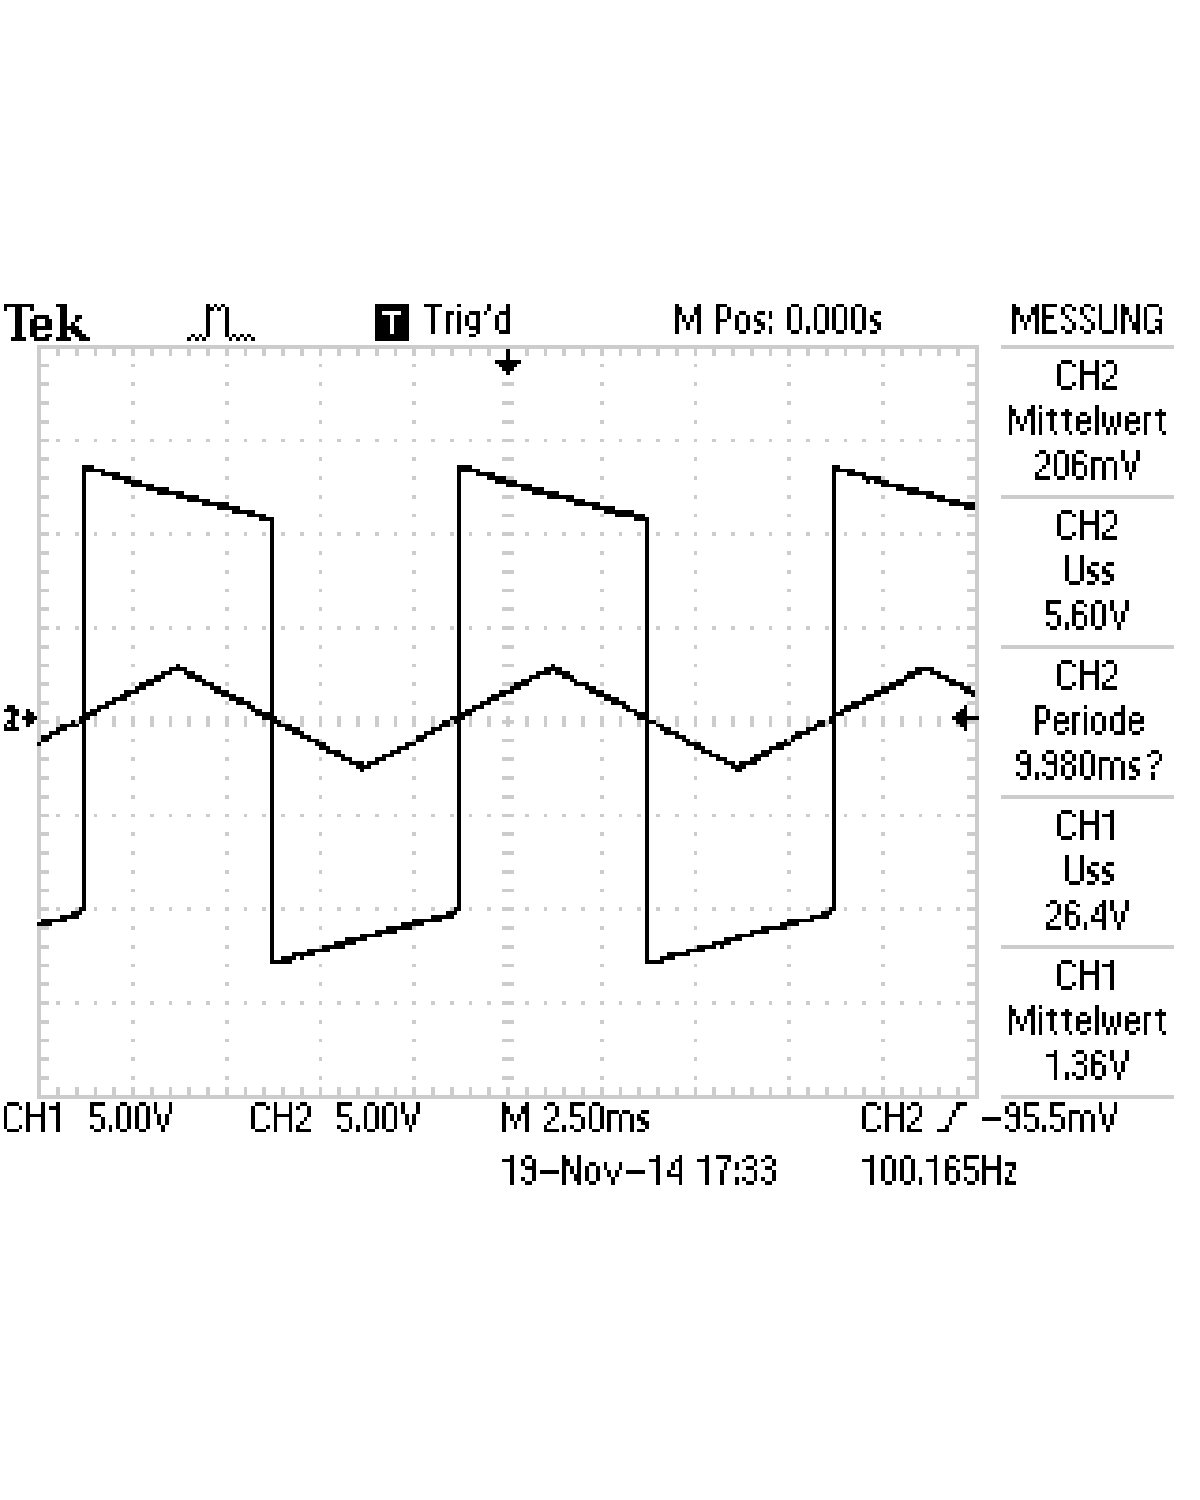
\includegraphics[width=\textwidth , scale = 0.4]{2_7_ohne_rf.pdf}
                \caption[Aufnahme des Signals ohne RF]{Aufnahme des Signals ohne RF}
  				\label{fig:2_7_ohne_rf}
        \end{subfigure}
        \caption{Op-Amp mit Hysterese}
        \label{fig:2_7}
\end{figure}

\subsection{Diskussion}
%(immer) die gemessenen werte und die bestimmten werte über die messfehler mit literaturwerten oder untereinander vergleichen
%in welchem fehlerintervall des messwertes liegt der literaturwert oder der vergleichswert?
%wie ist der relative anteil des fehlers am messwert und damit die qualität unserer messung?
%in einem satz erklären, wie gut unser fehler und damit unsere messung ist
%kurz erläutern, wie systematische fehler unsere messung beeinflusst haben könnten
%(wichtig) zum schluss ansprechen, in wie weit die ergebnisse mit der theoretischen vorhersage übereinstimmen
%--------------------------------------------------------------------------------------------
%falls tabellen mit den messwerten zu lang werden, kann die section mit den messwerten auch hinter der diskussion angefügt bzw. eine section mit dem anhang eingefügt werden.
%1-----------------------------------------------1

Bei der Rückkopplung durch RF ist der Effekt der Hysterese deutlich zu sehen, vgl. Abbildung \ref{fig:2_7}.

\section{Strommessung mit dem Op-Amp}
%kurz das ziel dieses versuchsteiles ansprechen, damit keine zwei überschriften direkt übereinander stehen!
%bei schwierigeren versuchen kann auch der theoretische hintergrund erläutert werden. (mit formeln, herleitungen und erklärungen)
Mit dem Op-Amp können verschiedene Schaltungen zur Messung kleiner Ströme aufgebaut werden.
\subsection{Verwendete Geräte}
%(immer) eine skizze oder ein foto einfügen, die geräte/materialien !nummerieren! und z.b. eine legende dazu schreiben, besser wäre es das ganze in einem Fließtext gut zu beschreiben.
%falls am anfang des versuches nicht klar ist, was alles verwendet wird, wenn möglich erst am ende ein großes foto von den verwendeten materialien machen!\\

Es werden ein Operationsverstärker, eine Photozelle, ein Widerstand und DVMs zur Messung verwendet.

\subsection{Versuchsaufbau}
%skizze zum versuchsaufbau (oder foto) einfügen,   es muss erklärt werden wie das ganze funktioniert und welche speziellen einstellungen verwendet wurden (z.b. welche knöpfe an den geräten für die messung verdreht wurden)

R ist Widerstand zwischen 100k$\Omega$ und 10M$\Omega$.

\begin{figure}[H] 
  \centering
    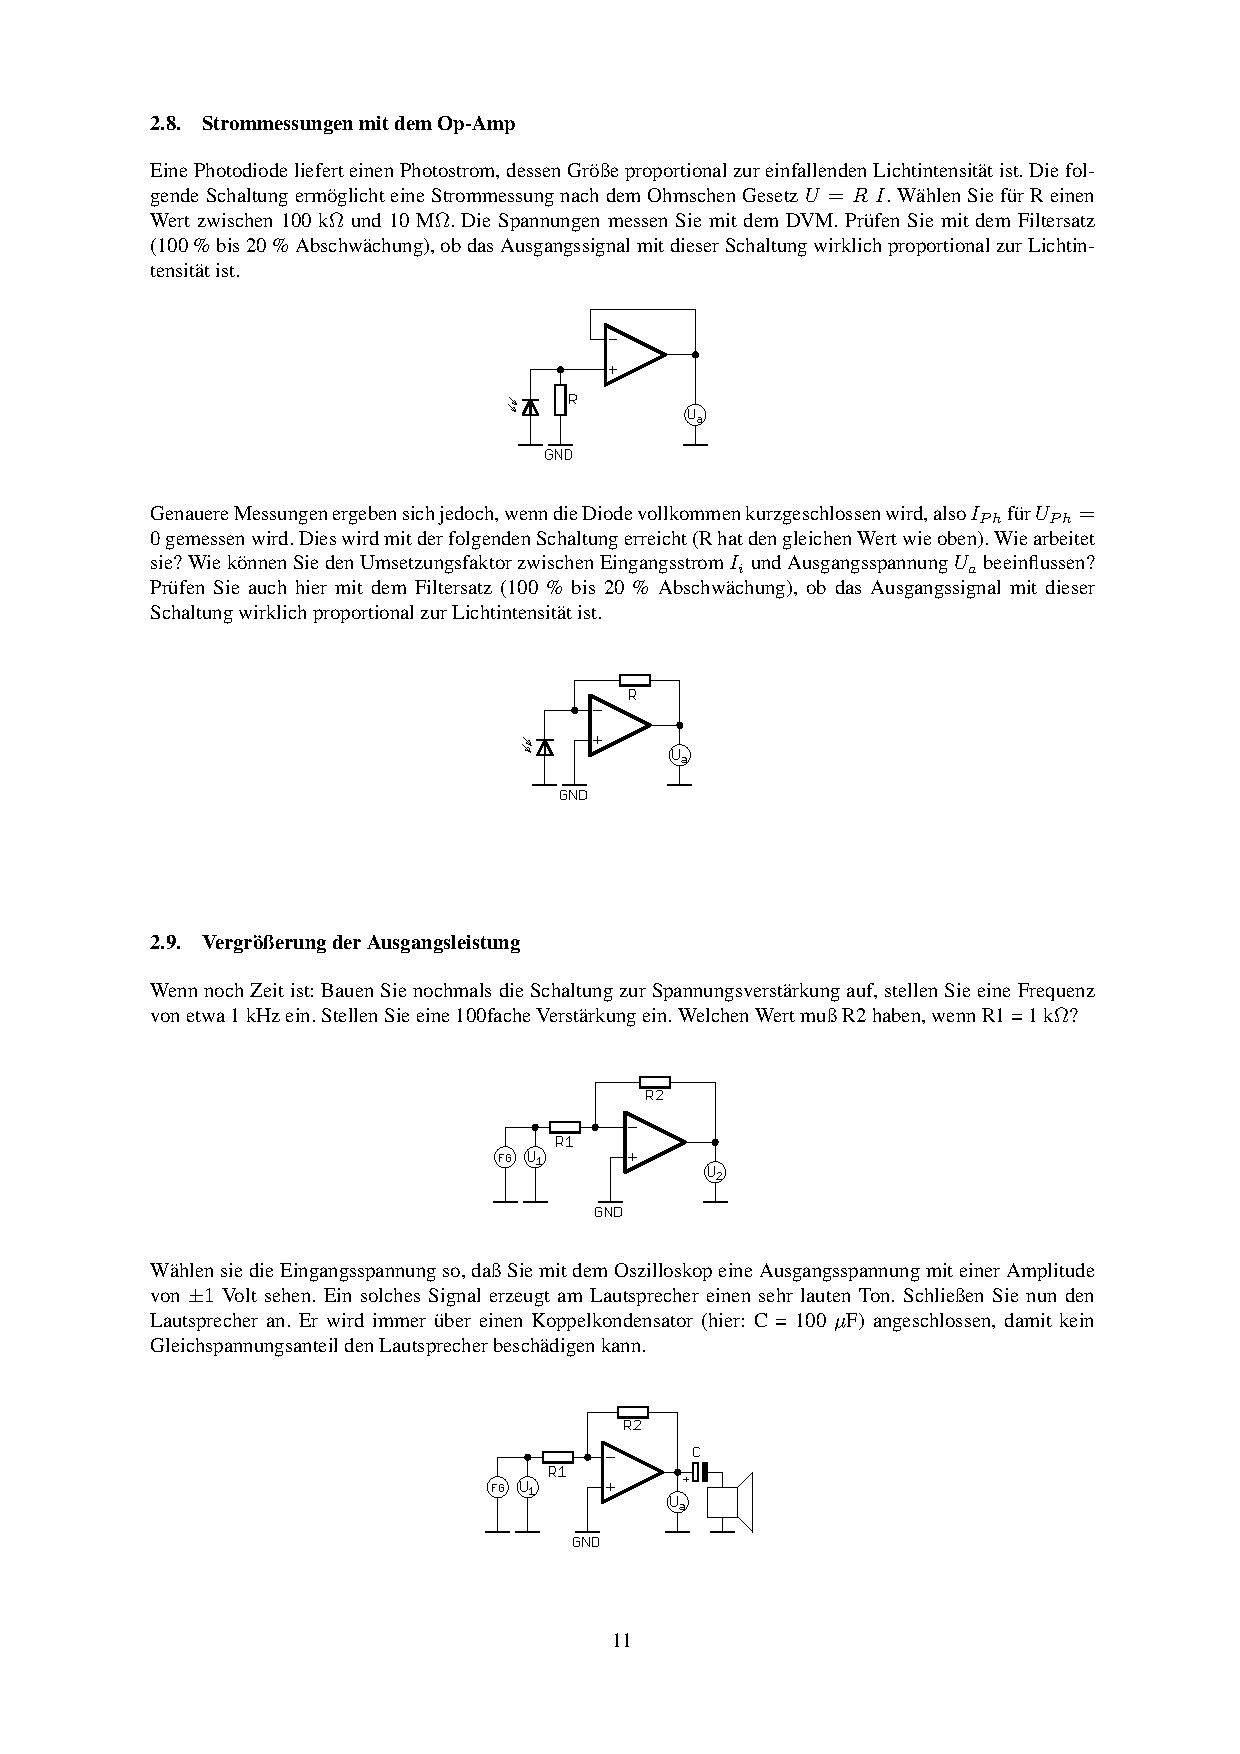
\includegraphics[trim = 10mm 215mm 10mm 50mm, clip, scale = 1]{ep4_14[Page11].pdf}
  	\caption[Schaltskizze für die Nutzung des Op\_Amp zur Strommessung]{Schaltskizze für die Nutzung des Op\_Amp zur Strommessung\footnotemark}
  \label{fig:1}
\end{figure}
\footnotetext{Abbildung entnommen von http://www.atlas.uni-wuppertal.de/$\sim$kind/ep4\_14.pdf Seite 11 am 17.11.2014}

Aufbau für bessere Messergebnisse, R ist immer noch ein Widerstand zwischen 100k$\Omega$ und 10M$\Omega$.

\begin{figure}[H] 
  \centering
    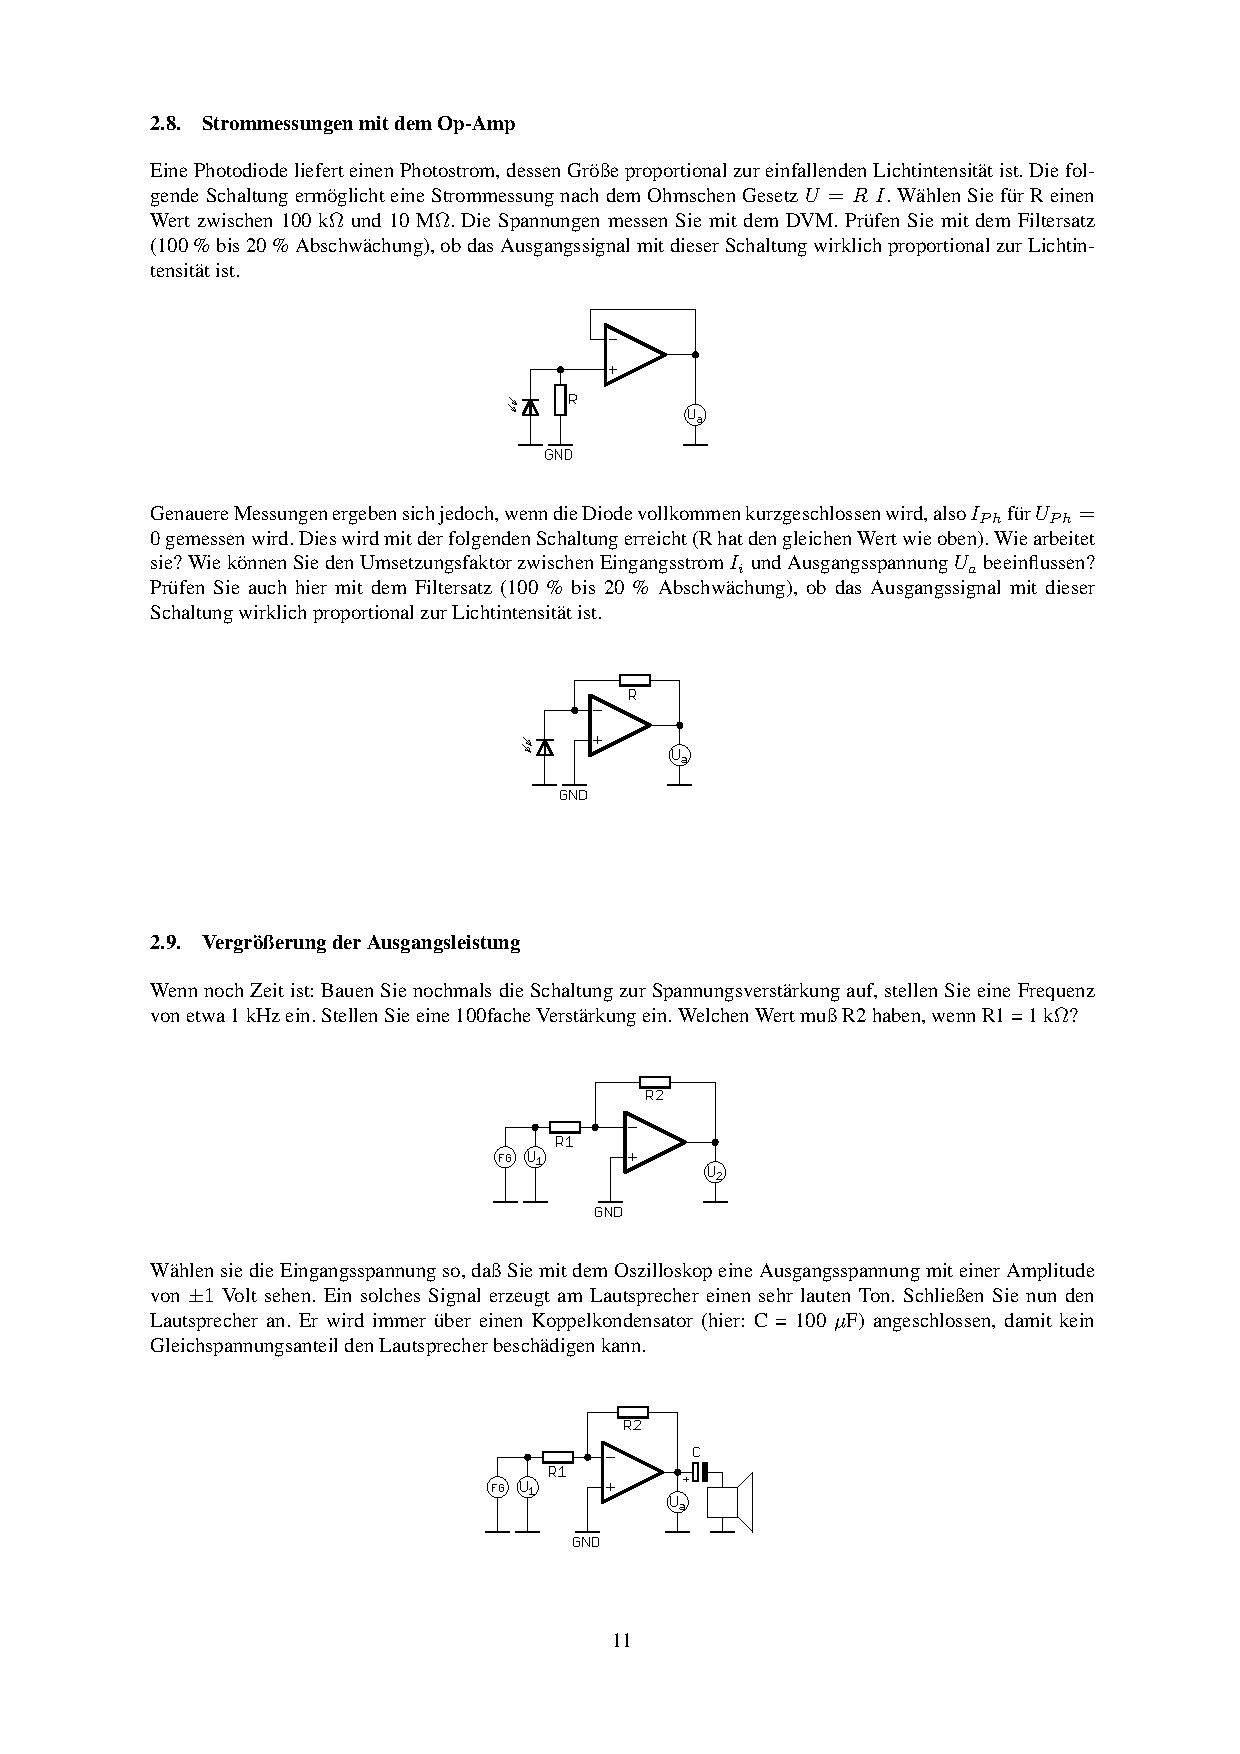
\includegraphics[trim = 10mm 155mm 10mm 110mm, clip, scale = 1]{ep4_14[Page11].pdf}
  	\caption[Schaltskizze für die Nutzung des Op\_Amp zur Strommessung]{Schaltskizze für die Nutzung des Op\_Amp zur Strommessung\footnotemark}
  \label{fig:1}
\end{figure}
\footnotetext{Abbildung entnommen von http://www.atlas.uni-wuppertal.de/$\sim$kind/ep4\_14.pdf Seite 11 am 17.11.2014}

\subsection{Versuchsdurchführung}
%erklären, !was! wir machen, !warum! wir das machen und mit welchem ziel
%(wichtig) präzize erklären, wie bei dem versuch vorgegangen und was gemacht wurde
In diesem Versuchsteil soll der Strom, der abhängig von der Lichtintensität von der Photodiode geliefert wird, gemessen werden. Dazu wird zuerst eine Schaltung aufgebaut, die eine Messung nach dem Ohmschen Gesetz erlaubt, und danach eine Schaltung, welche die Photodiode (fast) nicht belastet, sodass der Photostrom besser gemessen werden kann.
\subsection{Messergebnisse}
%die messwerte in !übersichtlichen! tabellen angegeben
%zu viele kleine tabellen in große tabellen überführen!
%zu große tabellen mit dem [scale]-befehl scalieren oder (falls zu lang) in zwei kleinere tabellen aufteilen
%(wichtig) vor !jeder! tabelle sagen, was gemessen wurde und wie die fehler gewählt wurden und ausreichend !erklären!, !warum! wir unsere fehler grade so gewählt haben

Der Fehler der Spannung wurde mit dem Angegebenem Fehler und der Ableseungenauigkeit bestimmt und beträgt 0,016.

\begin{table}[H]
\caption{Messdaten des ersten Aufbaus}
\begin{center}
\begin{tabular}{|r|r|}
\hline
\multicolumn{1}{|l|}{Intensität} & \multicolumn{1}{l|}{U\_0/V} \\ \hline
100 & 0,29 \\ \hline
80 & 0,27 \\ \hline
60 & 0,25 \\ \hline
40 & 0,22 \\ \hline
20 & 0,14 \\ \hline
0 & 0,01 \\ \hline
\end{tabular}
\end{center}
\label{tab:2_8_a}
\end{table}

Der Fehler der Spannung wurde mit dem Angegebenem Fehler und der Ableseungenauigkeit bestimmt und beträgt 0,016.

\begin{table}[H]
\caption{Messdaten des zweiten Aufbaus}
\begin{center}
\begin{tabular}{|r|r|}
\hline
\multicolumn{1}{|l|}{Intensität} & \multicolumn{1}{l|}{U\_0/V} \\ \hline
100 & 0,63 \\ \hline
80 & 0,53 \\ \hline
60 & 0,4 \\ \hline
40 & 0,28 \\ \hline
20 & 0,15 \\ \hline
0 & 0,01 \\ \hline
\end{tabular}
\end{center}
\label{tab:2_8_b}
\end{table}


\subsection{Auswertung}
%zuerst !alle! errechneten werte entweder in ganzen sätzen aufzählen, oder in tabellen (übersichtlicher) dargestellen, sowie auf die verwendeten formeln verweisen (die referenzierung der formel kann in der überschrift stehen)
%kurz erwähnen (vor der tabelle), warum wir das ganze ausrechnen bzw. was wir dort ausrechnen
%danach histogramme und plots erstellen, wobei wenn möglich funktionen durch die plots gelegt werden (zur not können auch splines benutzt werden, was aber angegeben werden muss)
%bei fits immer die funktion und das reduzierte chiquadrat mit angegeben, wobei auf verständlichkeit beim entziffern der zehnerpotenzen geachtet werden muss z.b. f(x)=(wert+-fehler)\cdot10^{irgendeine zahl}\cdot x + (wert+-fehler)\cdot10^{irgendeine zahl}
%bei jedem fit erklären, nach welchem zusammenhang gefittet wurde und warum!
%bei plots darauf achten, dass die achsenbeschriftung (auch die tics) die richtige größe haben und die legende im plot nicht die messwerte verdeckt
%kurz die aufgabenstellung abhandeln
%2-----------------------------------------------2

Im Versuchsteil 2.8 soll der Op-Amp zur Strommessung verwendet werden. Dazu wird eine Photodiode als Spannungsquelle verwendet und die Ausgangsspannung in Abhängigkeit der Intensität gemessen. Dabei sollte überprüft werden, ob die Ausgangsspannung proportional zur Intensität ist. Der Verlauf bei nicht kurzgeschlossener Photodiode, Abbildung \ref{fig:2_8_a} ist nicht linear, der bei kurzgeschlossener Photodiode schon, Abbildung \ref{fig:2_8_b}. Die Messdaten aus Tabelle \ref{tab:2_8_b} wurden mit einer linearen Funktion gefittet, das reduzierte Chi-Quadrat ergab sich mit 0,55 was den für einen starken linearen Zusammenhang spricht.

\begin{figure}[H]
        \centering
        \begin{subfigure}[b]{0.48\textwidth}
                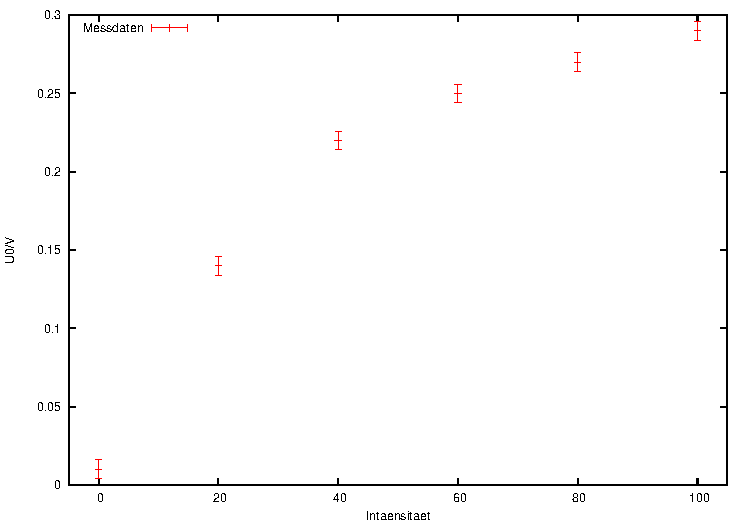
\includegraphics[width=\textwidth , scale = 0.4]{a_2_8_a.pdf}
                \caption[Plot der Messdaten ohne Kurzschluss der Diode]{Plot der Messdaten ohne Kurzschluss der Diode}
 				 \label{fig:2_8_a}
        \end{subfigure}%
        %~ %add desired spacing between images, e. g. ~, \quad, \qquad, \hfill etc.
          %(or a blank line to force the subfigure onto a new line)
        \hfill
        \begin{subfigure}[b]{0.48\textwidth}
                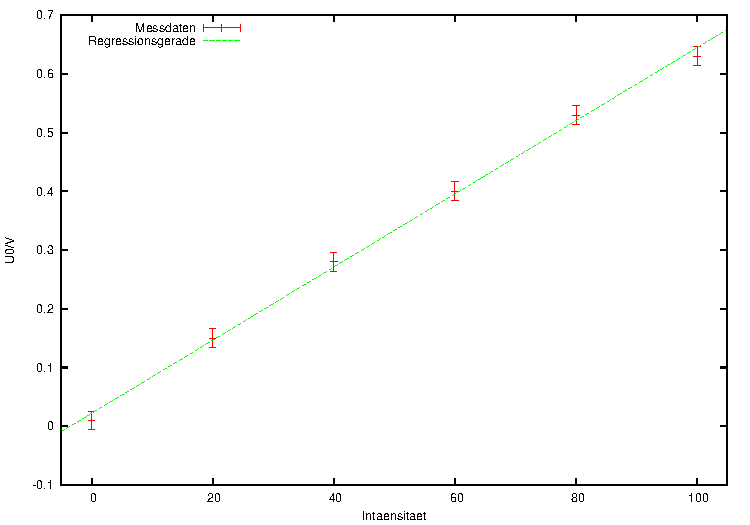
\includegraphics[width=\textwidth , scale = 0.4]{a_2_8_b.pdf}
                \caption[Plot der Messdaten mit Kurzschluss der Diode]{Plot der Messdaten mit Kurzschluss der Diode}
  				\label{fig:2_8_b}
        \end{subfigure}
        \caption{Plots der Messdaten mit/ohne Kurzschluss der Diode}
        \label{fig:2_8}
\end{figure}

\subsection{Diskussion}
%(immer) die gemessenen werte und die bestimmten werte über die messfehler mit literaturwerten oder untereinander vergleichen
%in welchem fehlerintervall des messwertes liegt der literaturwert oder der vergleichswert?
%wie ist der relative anteil des fehlers am messwert und damit die qualität unserer messung?
%in einem satz erklären, wie gut unser fehler und damit unsere messung ist
%kurz erläutern, wie systematische fehler unsere messung beeinflusst haben könnten
%(wichtig) zum schluss ansprechen, in wie weit die ergebnisse mit der theoretischen vorhersage übereinstimmen
%--------------------------------------------------------------------------------------------
%falls tabellen mit den messwerten zu lang werden, kann die section mit den messwerten auch hinter der diskussion angefügt bzw. eine section mit dem anhang eingefügt werden.
%1-----------------------------------------------1

Bei der Schaltung mit kurzgeschlossener Diode ergab sich der erwartet lineare Zusammenhang zwischen der Ausgangsspannung und der Intensität des einfallenden Lichts. Bei der Schaltung mit nicht kurzgeschlossener Photodiode ergab sich kein linearer Zusammenhang.

\section{Fazit}
%im fazit nochmal alles zusammenfassen und den verlauf der messung abschätzen
%gravierende sytematische probleme bei den messungen nochmal betonen und die wertigkeit unserer ergebnisse einordnen
Die Versuche haben die vielseitigen Einsatzmöglochkeiten des Op-Amps gezeigt, was ihn zu einem unverzichtbarem Element in der Netzwerktechnik macht. Mit ihm können Schaltungen zur Strommessung, Spannungsverstärkung und Pufferschaltungen mit nahezu idealen Eigenschaften konstruiert werden.

\end{document}

